\documentclass[preprint2,numberedappendix,tighten]{aastex6}  % USE THIS TO MAKE BIB, THEN FORMAT USING EMULATEAPJ
%\documentclass[twocolumn,numberedappendix]{emulateapj}
\shorttitle{Characterizing Signal Loss, Error, and Bias in the 21cm Reionization Power Spectrum}
\shortauthors{Cheng et al.}

\usepackage{amsmath}
\usepackage{graphicx}
\usepackage[figuresright]{rotating}
\usepackage{natbib}
\usepackage{ctable}
\usepackage{comment}
\usepackage{bm}
%\usepackage{mathtools}
\usepackage{xparse}
%\usepackage{titlesec}
\citestyle{aa}

\defcitealias{ali_et_al2015}{A15}

%Math stuff from Danny
\NewDocumentCommand{\evalat}{sO{\big}mm}{%
  \IfBooleanTF{#1}
   {\mleft. #3 \mright|_{#4}}
   {#3#2|_{#4}}%
}

%		Math Shortcuts from Adrian
%\def\b{\mathbf{b}}
%\def\k{\mathbf{k}}
%\def\r{\mathbf{r}}
%\def\q{\mathbf{q}}
%\def\b{\mathbf{b}}
%\def\kp{\mathbf{k}^\prime}
%\def\kpp{\mathbf{k}^{\prime\prime}}
%\def\V{\mathbb{V}}
%\def\At{\tilde{A}}
%\def\Vt{\tilde{V}}
%\def\Tt{\tilde{T}}
%\def\tb{\langle T_b\rangle}
%\newcommand{\vis}{\mathbf{v}}
\newcommand{\x}{\mathbf{x}}
\newcommand{\f}{\mathbf{f}}
\newcommand{\s}{\mathbf{s}}
\newcommand{\e}{\mathbf{e}}
\newcommand{\p}{\mathbf{p}}
\newcommand{\phat}{\widehat{\mathbf{p}}}
\newcommand{\C}{\mathbf{C}}
\newcommand{\Chat}{\mathbf{\widehat{C}}}
\newcommand{\F}{\mathbf{F}}
\newcommand{\Fhat}{\mathbf{\widehat{F}}}
\newcommand{\Q}{\mathbf{Q}}
\newcommand{\I}{\mathbf{I}}
%\newcommand{\xhat}{\widehat{\mathbf{x}}}
%\newcommand{\nhat}{\widehat{\mathbf{n}}}
%\newcommand{\A}{\mathbf{A}}
%\newcommand{\N}{\mathbf{N}}
%\newcommand{\rhat}{\widehat{\mathbf{r}}}
%\newcommand{\khat}{\widehat{\mathbf{k}}}
%\newcommand{\btheta}{\boldsymbol \theta}

\newcommand{\cc}[1]{{\color{purple} \textbf{[CC: #1]}}}
\newcommand{\acl}[1]{{\color{red} \textbf{[ACL:  #1]}}}
\newcommand{\dcj}[1]{{\color{orange} \textbf{[DCJ: #1]}}}
\newcommand{\mjk}[1]{ {\color{olive} \textbf{[MJK: #1]}} }
\newcommand{\jea}[1]{{\color{blue} \textbf{[JEA: #1]}} }
\newcommand{\jp}[1]{ {\color{pink} \textbf{[JCP: #1]}} } %y'all picked all the good colors

% Math shortcuts from James
\newcommand{\invC}{\ensuremath{\C^{-1}}}
\newcommand{\dC}[1]{\ensuremath{\C_{,#1}}}
\DeclareMathOperator{\Tr}{Tr}
\newcommand{\half}{\ensuremath{\frac{1}{2}}}
\newcommand{\PDeriv}[2]{\ensuremath{\frac{\partial #1}{\partial #2}}}

% Math shortcuts from Danny
\newcommand{\Prob}{\mathbf{P}}


\begin{document}
\title{Characterizing Signal Loss, Error, and Bias in the 21cm Reionization \\Power Spectrum: A Revised Study of PAPER-64}

\author{
Carina Cheng\altaffilmark{1}$^{,\diamond}$,
Aaron R. Parsons\altaffilmark{1,2},
Matthew Kolopanis \altaffilmark{3},
Daniel C. Jacobs\altaffilmark{3}, 
Adrian Liu\altaffilmark{1,4}$^{,\dagger}$, 
Saul A. Kohn\altaffilmark{5},
Jonathan C. Pober\altaffilmark{6}, 
James E.~Aguirre\altaffilmark{5},
Zaki S. Ali\altaffilmark{1}, 
Gianni Bernardi\altaffilmark{7,8,9}, 
Richard F. Bradley\altaffilmark{10,11,12},
Chris L. Carilli\altaffilmark{13,14},
David R. DeBoer\altaffilmark{2}, 
Matthew R. Dexter\altaffilmark{2},
Joshua S. Dillon\altaffilmark{1}$^{,*}$,
Pat Klima\altaffilmark{11},
David H. E. MacMahon\altaffilmark{2},
David F. Moore\altaffilmark{5},
Chuneeta D. Nunhokee\altaffilmark{8},
William P. Walbrugh\altaffilmark{7},
Andre Walker\altaffilmark{7}
}

\altaffiltext{1}{Astronomy Dept., U. California, Berkeley, CA}
\altaffiltext{2}{Radio Astronomy Lab., U. California, Berkeley CA}
\altaffiltext{3}{School of Earth and Space Exploration, Arizona State U., Tempe AZ}
\altaffiltext{4}{Berkeley Center for Cosmological Physics, Berkeley, CA} 
\altaffiltext{5}{Dept. of Physics and Astronomy, U. Penn., Philadelphia PA} 
\altaffiltext{6}{Dept. of Physics, Brown University, Providence RI}
\altaffiltext{7}{Square Kilometer Array, S. Africa, Cape Town South Africa}
\altaffiltext{8}{Dept. of Physics and Electronics, Rhodes University, South Africa}
\altaffiltext{9}{INAF-Instituto di Radioastronomia, Bologna Italy}
\altaffiltext{10}{Dept. of Electrical and Computer Engineering, U. Virginia, Charlottesville VA}
\altaffiltext{11}{National Radio Astronomy Obs., Charlottesville VA}
\altaffiltext{12}{Dept. of Astronomy, U. Virginia, Charlottesville VA}
\altaffiltext{13}{National Radio Astronomy Obs., Socorro NM}
\altaffiltext{14}{Cavendish Lab., Cambridge UK}

%		Notes	
	
%Reference section with: \ref{sec:Intro}
%Reference equation with: \eqref{eq:eqtest}
%Reference figure with: \ref{fig:figtest}
%Cite paper inside sentence: \citet{ref}
%Cite paper at end of sentence: \citep{ref}
%Cite paper inside a parenthetical sentence: \citealt{ref}

%To compile with references shown, compile in BibTeX once and LaTeX twice


%		Sample Equation Syntax
%\begin{equation}
%\label{eqtest}
%\langle \widetilde{T} (\mathbf{k}) \widetilde{T}^* (\mathbf{k^\prime}) \rangle = (2 \pi)^3 \delta^D (\mathbf{k} - \mathbf{k}^\prime) P(k),
%\end{equation}


% ABSTRACT ---------------------------------------------------------------------------------

\begin{abstract}
The Epoch of Reionization (EoR) is an uncharted era in our Universe's history during which the first stars and 
galaxies led to the ionization of neutral hydrogen in the intergalactic medium. There are many experiments investigating the 
EoR by tracing the 21\,cm line of neutral hydrogen, a signal which is very faint and difficult to isolate. With a new generation 
of instruments and a statistical power spectrum detection in our foreseeable future, it has become increasingly important to 
develop techniques that help maximize sensitivity while validating results. Additionally, it is imperative to understand the trade-offs 
between different methods and their effects on power spectrum estimates. In this paper, we focus on three major 
themes --- signal loss, power spectrum error estimation, and bias in measurements. We describe techniques that affect 
these themes using both toy models and data taken by the 64-element configuration of the Donald C. Backer Precision Array 
for Probing the Epoch of Reionization (PAPER). In particular, we highlight how detailed investigations of these themes have 
led to a revised, higher 21\,cm power spectrum upper limit from PAPER-64. This revised result, presented in a companion paper by Kolopanis et al. (\textit{submitted}), mostly stems from an 
improved signal loss calculation for loss associated with empirically estimated covariances and supersedes results from 
previously published PAPER analyses.
\end{abstract}

% INTRO ---------------------------------------------------------------------------------

\section{Introduction}
\label{sec:Intro}

{\let\thefootnote\relax\footnote{$^{\diamond}$\href{mailto:ccheng@berkeley.edu}{ccheng@berkeley.edu}}}
{\let\thefootnote\relax\footnote{$^{\dagger}$Hubble Fellow}}
{\let\thefootnote\relax\footnote{$^{*}$NSF AAPF Fellow}}
\setcounter{footnote}{0}

By about one billion years after the Big Bang ($z \sim 6$), the first stars and galaxies are thought to have ionized all the 
neutral hydrogen that dominated the baryonic matter content in the Universe. This transition period, during which the first 
luminous structures formed from gravitational collapse and began to emit intense radiation that ionized the cold neutral gas 
into a plasma, is known as the Epoch of Reionization (EoR). The EoR is a relatively unexplored era in our \textit{cosmic dawn}, which spans the birth of the first stars to the full reionization of the intergalactic medium (IGM). Its 
history encodes important information regarding the nature of the first galaxies and the processes of structure formation. 
Direct measurements of the EoR would unlock powerful characteristics about the IGM, revealing connections 
between the matter distribution exhibited via cosmic microwave background (CMB) studies and the highly structured 
web of galaxies we observe today (for a review, see \citet{barkana_and_loeb2001}, \citet{furlanetto_et_al2006} and \citet{loeb_furlanetto_2013}).

One promising technique to probe the EoR is to target the 21\,cm wavelength signal that is emitted and absorbed by neutral hydrogen via 
its spin-flip transition (\citealt{furlanetto_et_al2006}; \citealt{barkana_and_loeb2008}; \citealt{morales_and_wyithe2010}; \citealt{pritchard_and_loeb2010}; \citealt{pritchard_loeb2012}). This technique is powerful because it can be observed both spatially and as a function of redshift --- that is, the wavelength 
of the signal reaching our telescopes can be directly mapped to a distance from where the emission originated before 
stretching out as it traveled through expanding space. 21\,cm tomography offers a unique window into the 
evolution of ionization, temperature, and density fluctuations.

In addition to the first tentative detection of the EoR signal made by the Experiment to Detect the Global EoR Signature (EDGES; \citealt{bowman_et_al2018}; \citealt{bowman2010}), there are several radio telescope experiments that have succeeded in using 
the 21\,cm signal from hydrogen to place constraints on the brightness of the signal. Examples of experiments investigating the 
mean brightness temperature of the EoR relative to the CMB are the Large Aperture Experiment to Detect the Dark Ages (LEDA; \citealt{bernardi_et_al2016}), the 
Dark Ages Radio Explorer (DARE; \citealt{burns2012}), the Sonda Cosmol\'ogica de las Islas para la Detecci\'on de 
Hidr\'ogeno NeutroSciHi (SCI-HI; \citealt{voytek2014}), the Broadband Instrument for Global HydrOgen ReioNisation Signal 
(BIGHORNS; \citealt{sokolowski2015}), and the Shaped Antenna measurement of the background RAdio Spectrum (SARAS; 
\citealt{patra2015}). Radio interferometers which seek to measure statistical power spectra include the Giant Metre-wave 
Radio Telescope (GMRT; \citealt{paciga_et_al2013}), the LOw Frequency ARray (LOFAR; \citealt{van_haarlem_et_al2013}), 
the Murchison Widefield Array (MWA; \citealt{tingay_et_al2013}), the 21 Centimeter Array (21CMA; 
\citealt{peterson_et_al2004}; \citealt{wu2009}), the Square Kilometre Array (SKA; \citealt{koopmans_et_al2015}), and PAPER (\citealt{parsons_et_al2010}). The Hydrogen Epoch of 
Reionization Array (HERA), which is currently being built, is a next-generation instrument that aims to combine lessons 
learned from previous experiments and is forecast to be able to make a high-significance power spectrum 
detection with an eventual $350$ elements using current analysis techniques (\citealt{pober_et_al2014}; \citealt{liu_parsons_2016}; \citealt{dillon_parsons2016}; \citealt{deboer_et_al2017}).

The major challenge that faces all 21\,cm experiments is isolating a small signal that is buried underneath foregrounds and 
instrumental systematics that are, when combined, four to five orders of magnitude brighter \citep[e.g.,][]{santos_et_al2005, ali_et_al2008, deOliveiraCosta_et_al2008, jelic_et_al2008, bernardi_et_al2009, bernardi_et_al2010, ghosh_et_al2011, pober_et_al2013b, bernardi_et_al2013, dillon_et_al2014, kohn_et_al2016}. A clean measurement therefore requires an intimate understanding of the instrument and a rigorous study of data analysis choices. With continual progress being made 
in the field and HERA on the horizon, it is becoming increasingly important to understand how the methods we choose interact 
with each other to affect power spectrum results. More specifically, it is imperative to develop techniques and tests that ensure 
the accuracy and reliability of a potential EoR detection. In this paper, we discuss three topics (signal loss, error estimation, and bias) that are essential to investigate 
for a robust 21\,cm power spectrum analysis. We also highlight four power spectrum techniques (fringe-rate filtering, weighting, bootstrapping, jackknife testing) and their trade-offs, potential 
pitfalls, and connections to the themes. We first approach the themes from a broad perspective, and then perform a detailed 
case study using data from the 64-element configuration of PAPER. In this study we use a subset of the PAPER-64 data to illustrate our revised analysis methods, while a companion paper, Kolopanis et al. (\textit{submitted}), builds off of the methods in this paper to present revised PAPER-64 results for multiple redshifts and baseline types.

Finally, this paper adds to the growing foundations of lessons which have been documented, for example, in \citet{Paciga2013}, \citet{Patil2016}, and \citet{Jacobs2016}, by the GMRT, LOFAR, and MWA projects respectively. These lessons are imperative as the community as a whole moves towards higher sensitivities and potential EoR detections.

This paper is organized into two main halves. In Section \ref{sec:Themes} we introduce the three themes of our focus, using a 
toy model to develop intuition for each one. In Section \ref{sec:CaseStudy} we present a case study into each theme using data 
from the PAPER-64 array, highlighting key changes from the previously published result in \citet{ali_et_al2015}, henceforth known as \citetalias{ali_et_al2015}, which have led to a 
revised PAPER-64 power spectrum result (Kolopanis et al. (\textit{submitted})). We conclude in Section \ref{sec:Con}.

% SECTION 2 INTRO ---------------------------------------------------------------------------------

\section{Power Spectrum Themes and Techniques}
\label{sec:Themes}

There are many choices a 21\,cm data analyst must consider. %For PAPER, its grid configuration allows the use of many signal processing tricks to down-weight foregrounds without reference to a sky model. However, even with the advantage of being agnostic about the sky, many questions still remain.
%, though the space is significantly constrained by 
%the type of instrument being used.  The PAPER instrument in its grid configuration focuses most sensitivity on 
%only a few baselines but imaging performance is poor. In this space, signal processing tricks which filter or 
%down-weight foreground modes without reference to a sky model have the advantage of being agnostic about 
%the sky. However, even within this problem sub-space, questions remain.
How can time-ordered measurements be combined? How can the 
variance of the data be estimated? In what way(s) can the data be weighted to suppress contaminated modes while not 
destroying an EoR signal? How can a statistically significant detection of a signal be properly identified? Many common techniques, such as 
averaging data, weighting, bootstrapping, and jackknife testing, address these issues but harbor additional trade-offs. For 
example, an aggressive filtering method may succeed in eliminating interfering systematics but comes at the cost of losing 
some EoR signal. A chosen weighting scheme may theoretically maximize sensitivity but fail to suppress foregrounds in practice. 

Though there are many data analysis choices, measuring the statistical 21\,cm power spectrum ultimately requires robust 
methods for determining accurate confidence intervals and rigorous techniques to identify and control systematics.  In this 
paper, we focus on three 21\,cm power spectrum themes that encapsulate this goal and discuss four techniques that interplay 
with each other and impact the themes. We will give brief definitions now, and build intuition for each theme in the sections to 
follow.

\begin{center}
Power Spectrum Themes
\end{center}

A deep understanding of the following three themes is essential for the accuracy and interpretation of a 21\,cm power 
spectrum result. Stemming from a re-analysis of PAPER-64 data, we believe these themes serve as an important checklist for 
a rigorous power spectrum analysis.
\begin{itemize}
\item \textbf{Signal Loss} (Section \ref{sec:SiglossOverview}): Signal loss refers to attenuation of the target \textit{cosmological} signal 
in a power spectrum estimate. Certain analysis techniques can cause this loss, and if the amount of loss is not quantified accurately, it could lead to false non-detections and overly aggressive upper limits. Determining whether an analysis pipeline is lossy, and estimating the amount of loss if so, has subtle challenges but is necessary to ensure the accuracy of any result. 
\item \textbf{Error Estimation} (Section \ref{sec:ErrorOverview}): Confidence intervals on a 21\,cm power spectrum result 
determine the difference between a detection and a null result, which have two very different implications. Additionally, accurate error estimation is crucial for the comparison of results to theoretical models. Errors can be 
estimated in a variety of ways, and we will discuss a few of them.
\item \textbf{Bias} (Section \ref{sec:BiasOverview}): There are several possible sources of power offset in a visibility 
measurement that can show up as a detection in a power spectrum, such as bias from noise and foregrounds. In particular, a 
successful EoR detection would also imitate a bias. Proving that a bias is an EoR detection may be the most difficult challenge for 21\,cm 
analyses, as it is crucial to be able to distinguish a detection of foreground leakage, for example, from that of EoR. In this paper 
we will highlight some sources of bias, discuss ways to mitigate their effects, and describe tests that a true EoR detection must 
pass.
\end{itemize}

\begin{center}
Power Spectrum Techniques
\end{center}

The following techniques each have advantages when it comes to maximizing sensitivity and understanding systematics in 
data. However, some have limitations, and we will discuss circumstances in which there are trade-offs. We choose to focus on 
these four techniques because they represent major steps in PAPER's power spectrum pipeline, with several of them also 
being standard steps in general 21\,cm analyses.
\begin{itemize}
\item \textbf{Fringe-rate filtering:} Fringe-rate filtering is an averaging scheme for time-ordered data 
(\citealt{parsons_et_al2016}). Broadly, a fringe-rate filter averages visibilities in time to produce a smaller number of more sensitive 
independent samples. However, such a filter also affects the presence 
of foregrounds and systematics. We explain the trade-offs of filtering in more detail in Section \ref{sec:toymodel_frf}.
\item \textbf{Weighting:} A dataset can be weighted to emphasize certain features and minimize others. One particular flavor of 
weighting employed by previous PAPER analyses is inverse covariance weighting in frequency, which is a generalized version of inverse variance 
weighting that also takes into account frequency correlations (\citealt{liu_tegmark2011}; \citealt{dillon_et_al2013a}; \citealt{liu_et_al2014a}; \citealt{liu_et_al2014b}; \citealt{dillon_et_al2014}; \citealt{dillon_et_al2015}). Using such a technique enables the down-weighting of contaminant modes that obey a different covariance structure from that of cosmological modes. However, a challenge of inverse covariance 
weighting is in estimating a covariance matrix that is closest to the true covariance of the data; the discrepancy between the two has large impacts on signal loss. We investigate the impact of different types of weighting on signal loss in Section \ref{sec:SiglossOverview}.
\item \textbf{Bootstrapping:} In addition to using theoretical models for covariance matrices and theoretical error estimation 
methods, bootstrapping is one way to estimate errors. Namely, bootstrapping is a useful method for estimating errors of a dataset from 
itself (\citealt{andrae2010}). By randomly drawing many subsamples of the data, we obtain a sense of its inherent variance, though there are subtleties to 
consider such as the independence of values in a dataset. We explore this potential pitfall of bootstrapping in Section \ref{sec:ErrorOverview}.
\item \textbf{Jackknife testing:} A resampling technique useful for estimating bias, jackknives can be taken along different 
dimensions of a dataset to cross-validate results. In particular, null tests can be used to verify whether results are free of 
systematics, as done with CO power spectra (\citealt{keating_et_al2016}) and CMB measurements (see e.g. \citealt{ade_et_al2008}; \citealt{chiang_et_al2010}; \citealt{bischoff_et_al2011}; \citealt{das_et_al2011b}; \citealt{araujo_et_al2012}; \citealt{crites_et_al2015}; \citealt{ade_et_al2016}; \citealt{ade_et_al2017}; \citealt{sherwin_et_al2017}). An EoR detection must pass both jackknife and null tests, which we highlight in Section \ref{sec:JackknifeOverview}.
\end{itemize}

In the next three subsections, we study each theme in depth, focusing on how power spectrum technique trade-offs affect each. 
We use a toy data model to develop intuition into why certain analysis choices may be appealing and discuss ways in which 
they are limited. We highlight problems that can arise regarding each theme and offer suggestions to mitigate the issues. 
Ultimately, we show that rigorous investigations into signal loss, error estimation, and bias must be performed for robust 21\,cm results.

% SECTION 2 SIGLOSS ---------------------------------------------------------------------------------

\subsection{Signal Loss}
\label{sec:SiglossOverview}

Signal loss can arise in a variety of ways in the analysis pipeline, such as by fitting a polynomial during 
spectral calibration, applying a delay-domain filter, or deriving weights from data and applying them to itself. Here we focus on signal loss associated with 
applying a weighting matrix to data, a loss that can be significant depending on the choice of weighting and one that was 
previously underestimated in the \citetalias{ali_et_al2015} analysis.

Driven by the need to mitigate foreground bias, PAPER's previous analyses use a weighting method that aims to down-weight 
foregrounds. This weighting is applied to data, which is then propagated into a final estimator using the power spectrum 
estimation technique of quadratic estimators (QE) as done in \citet{liu_tegmark2011}, \citet{dillon_et_al2013a}, \citet{liu_et_al2014a}, \citet{liu_et_al2014b}, \citet{trott_et_al2012}, \citet{dillon_et_al2014}, \citet{dillon_et_al2015}, \citet{switzer_et_al2015}, and \citet{trott_et_al2016}. Before showing 
how signal loss can arise when using different weighting matrices, we first summarize QE as performed in the PAPER 
analysis.

We begin with our data vector, $\textbf{x}$, which contains our measured visibilities for a single baseline in Jy. It has length $N_{t}N_{f}$, but in practice we manipulate it as an array with dimensions ($N_{f}, N_{t}$), where 
$N_{t}$ is the number of time integrations and $N_{f}$ is the number of frequency channels. Visibilities are measurements of 
the Fourier transform of the sky along two spatial dimensions (using the flat-sky approximation), and since we are interested in three-dimensional Fourier modes 
we only need to take one Fourier transform of our visibilities along the line-of-sight dimension. We do this when forming the un-normalized power spectrum estimate $\widehat{q}_{\alpha}$:

\begin{equation}
\label{eq:qhat}
\widehat{q}_{\alpha} = \frac{1}{2}\textbf{x}^{\dagger}\textbf{R}\textbf{Q}^{\alpha}\textbf{R}\textbf{x}.
\end{equation}
Here, \noindent $\textbf{Q}$ is a family of matrices that takes our frequency-domain visibilities and Fourier transforms them, while also converting from Jy to 
Kelvin and taking into account cosmological scalings. It is formally evaluated as $\textbf{Q}^{\alpha} \equiv \frac{\partial\textbf{C}}{\partial p_{\alpha}}$ (which has dimensions ($N_{f}$,$N_{f}$)), or the derivative of the covariance $\textbf{C} \equiv \langle\textbf{x}\textbf{x}^{\dagger}\rangle$ with respect to the true bandpower $p_\alpha$, where $\alpha$ indexes a waveband in $k_{\parallel}$ (a cosmological wavenumber $k_{\parallel}$ is the 
Fourier dual to frequency under the delay approximation (\citealt{parsons_et_al2012b}), which is a good approximation for the short baselines that PAPER analyzes). $\textbf{R}$ is a weighting matrix with dimensions ($N_{f}$,$N_{f}$) --- as 
an example, inverse covariance weighting (the optimal form of QE) would set $\textbf{R} \equiv \textbf{C}^{-1}$ and a uniform-weighted case would use $
\textbf{R} \equiv \textbf{I}$, the identity matrix.

We normalize our power spectrum estimates using the matrix $\textbf{M}$:

\begin{equation}
\label{eq:phat}
\widehat{\textbf{P}} = \textbf{M}\widehat{\textbf{q}},
\end{equation}

\noindent where $\widehat{\textbf{P}}$ is the estimate of the true power spectrum $\textbf{P}$. The data analyst has a choice for $
\textbf{M}$. For simplicity in this section we choose $\textbf{M}$ to be diagonal, although we explore other cases for the analysis 
of PAPER-64 data as explained in Section \ref{sec:Bias}, subject to the constraint that each element of $\widehat{\textbf{P}}$ is a weighted sum of the elements of $\textbf{P}$ with weights that sum to unity.

In the next three sections, we use toy models to investigate the effects of weighting matrices on signal loss by experimenting with different matrices $\textbf{R}$ and examining their impact on the resulting power spectrum estimates $\widehat{\textbf{P}}$. Our goal in 
experimenting with weighting is to suppress foregrounds and investigate EoR losses associated with it. We note that we 
purposely take a thorough and pedagogical approach to describing the toy model examples given in the next few sections. The specifics of how signal loss appears in PAPER's analysis is later described in Section 
\ref{sec:Sigloss}.

\subsubsection{Toy Model: Inverse Covariance Weighting}
\label{sec:toymodel}

One choice for the weighting matrix $\textbf{R}$ used in power spectrum analysis is an inverse covariance matrix. This type of weighting is attractive for power spectrum analyses because it yields the smallest possible error bars on a measurement. Said differently, it gives the minimum variance estimate of the power spectrum (\citealt{tegmark_et_al1997a}; \citealt{bond_et_al1998}). In \citet{liu_tegmark2011}, it was shown that inverse covariance weighting also serves as a way to down-weight some portion of foregrounds (namely, those which do not share the same covariance structure as the cosmological signal), motivating our use of the weighting for previous PAPER analyses.

One important feature of weighting data by its true inverse covariance is that, while it can suppress some foregrounds, it cannot suppress the EoR signal (nor foreground modes that masquerade as signal-like modes). By construction, inverse covariance weighting in the quadratic estimator does not lead to signal loss. Therefore, in an ideal world with perfect foreground, 
instrumental, and EoR models, we could form $\textbf{C}$ in a way that accurately describes our measured data and use inverse covariance weighting to produce minimum variance power spectrum estimates without destroying the signal. In other words, the optimal quadratic estimator is by construction an unbiased estimator of the power spectrum.

In practice, we do not have perfect models for $\textbf{C}$, and it is the use of an estimated covariance $\widehat{\textbf{C}}$ instead of the true covariance $\textbf{C}$ that can lead to loss. We will now build intuition into how empirically estimated inverse covariance weighting can give rise to signal loss through the use of a toy model.

We construct a simple dataset that contains visibility data with $100$ time 
integrations and $20$ frequency channels. This model represents realistic dimensions of about an hour of PAPER data which 
might be used for a power spectrum analysis. For PAPER-64 (both the \citetalias{ali_et_al2015} analysis and our new analysis) we use $\sim8$ hours of data (with channel 
widths of $0.5$ MHz and integration times of $43$ seconds), but here we scale it down with no loss of 
generality. 

We create mock visibilities, $\textbf{x}$, and assume a non-tracking, drift-scan observation. Hence, flat spectrum sources (away 
from zenith) lead to measured visibilities which oscillate in time and frequency. We therefore form a mock visibility measurement of a bright foreground signal, $
\textbf{x}_{\rm FG}$, as a complex sinusoid that varies smoothly in time and frequency, a simplistic but realistic representation of a 
single bright source. We also create a mock visibility measurement of an EoR signal $\textbf{x}_{\rm EoR}$ as a complex, Gaussian random signal. A more 
realistic EoR signal would have a sloped power spectrum in $p(k)$ (instead of flat, as in the case of white noise), 
which could be simulated by introducing frequency correlations into the mock EoR signal. However, here we treat all 
$k$'s separately, so a simplistic white noise approximation can be used. Our combined data matrix is then $\textbf{x} = 
\textbf{x}_{\rm FG} + \textbf{x}_{\rm EoR}$, to which we apply different weighting schemes throughout Section \ref{sec:SiglossOverview}. The three data components are shown in Figure 
\ref{fig:toy_sigloss1}. 

\begin{figure}
	\centering
	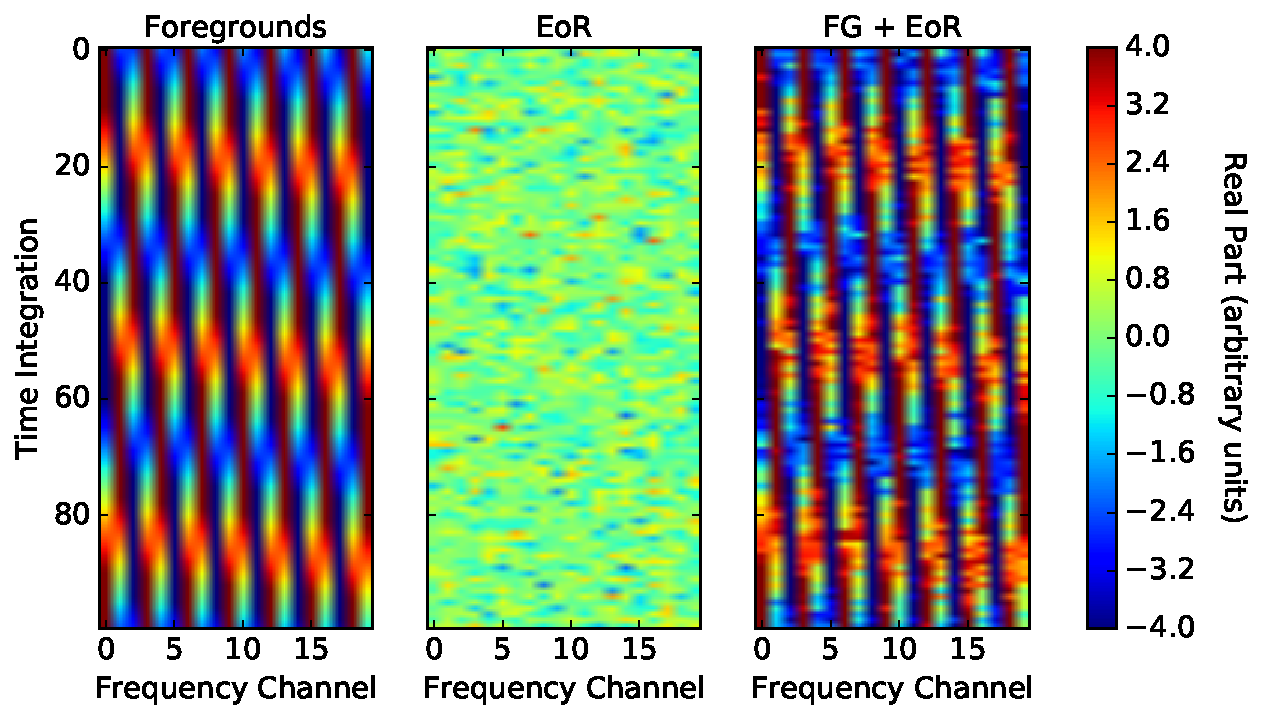
\includegraphics[trim={0cm 0cm 0cm 0cm},clip,width=\columnwidth]{plots/toy_sigloss1.pdf}
	\caption{Our toy model dataset to which we apply different weighting schemes to in order to investigate signal loss. We model a mock foreground-only visibility with a sinusoid signal that varies smoothly in 
time and frequency. We model a mock visibility of an EoR signal as a random Gaussian signal. We add the two together to form $\textbf{x} = 
\textbf{x}_{\rm FG} + \textbf{x}_{\rm EoR}$. Real parts are shown here.}
	\label{fig:toy_sigloss1}
\end{figure}

Without a perfect model for the covariance matrix $\textbf{C}$ of our data, one attractive way to estimate it is to empirically derive it from the data $\textbf{x}$ itself. Similar types of weightings that are based on variance information in data are done in \citet{chang_et_al2010} and \citet{switzer_et_al2015}. In previous PAPER analyses, one time-averages the data such that:

\begin{equation}
\widehat{\textbf{C}} \equiv \langle\textbf{xx}^{\dagger}\rangle_{t},
\end{equation}

\noindent assuming $\langle\textbf{x}\rangle_{t} = 0$ (a reasonable assumption since fringes average to $0$ over a sufficient 
amount of time), where $\langle \rangle_{t}$ denotes a finite average over time. The weighting matrix for our empirically estimated inverse covariance weighting is then $
\textbf{R} \equiv \widehat{\textbf{C}}^{-1}$.

First, we compute the power spectrum of our toy model dataset $\textbf{x}$ using QE formalism and $\textbf{R} \equiv \widehat{\textbf{C}}^{-1}$. 
The result is shown in green in the left plot of Figure \ref{fig:toy_sigloss3}. Also plotted in the figure are the uniform-weighted ($\textbf{R} \equiv \textbf{I}$) power spectrum of the individual components $
\textbf{x}_{\rm FG}$ (blue) and $\textbf{x}_{\rm EoR}$ (red). 

\begin{figure*}
	\centering
	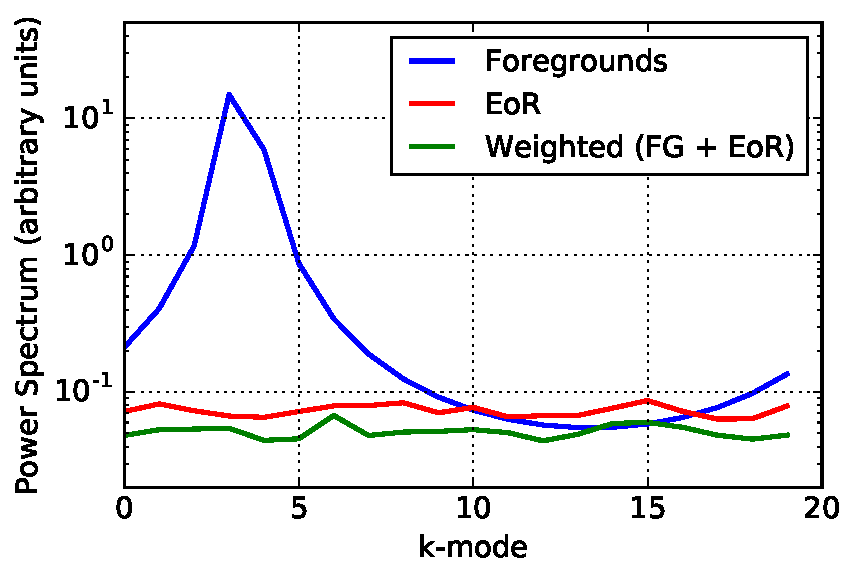
\includegraphics[trim={0cm 0cm 0cm 0cm},clip,height=0.33\textwidth]{plots/toy_sigloss3.pdf}
	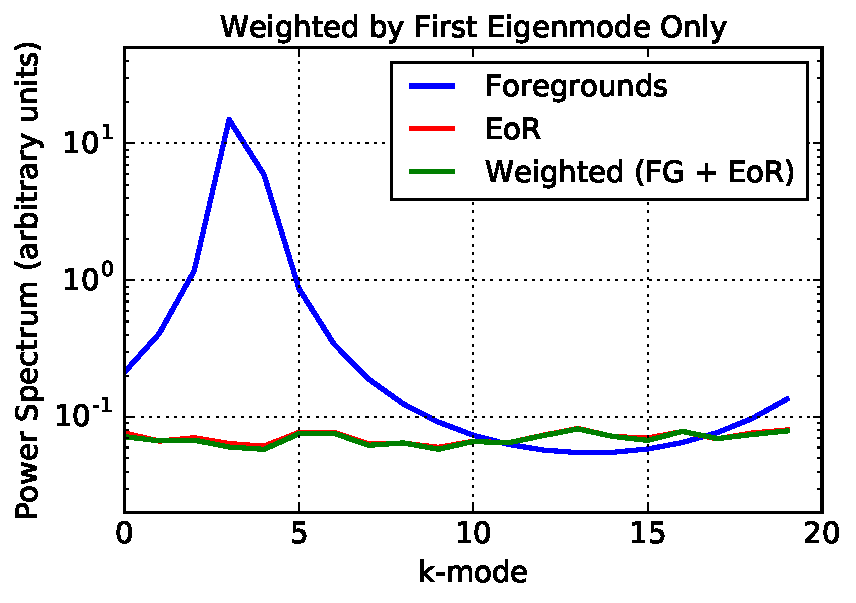
\includegraphics[trim={0cm 0cm 0cm 0cm},clip,height=0.33\textwidth]{plots/toy_sigloss4.pdf}
	\caption{Resulting power spectrum estimates for the toy model simulation described in Section \ref{sec:toymodel} --- 
foregrounds only (blue), EoR only (red), and the weighted FG + EoR dataset (green). The power spectrum of foregrounds peaks at a $k$-mode based on the frequency of the sinusoid used to create the mock FG signal. In the two panels, we compare empirically estimated inverse covariance weighting 
where $\textbf{C}$ is derived from the data (left), and projecting out the first eigenmode only (right). In the former 
case, signal loss arises from the coupling of the eigenmodes of $\widehat{\textbf{C}}$ to the data. For an empirically estimated $\widehat{\textbf{C}}$, its eigenvalues differ from those of the true covariance, where the coupling between EoR-dominated eigenmodes and the data can lead to loss.
Hence, there is negligible signal loss when assigning identical weights to all eigenmodes except the first, since we are only down-weighting the FG-dominating mode in this case.}
	\label{fig:toy_sigloss3}
\end{figure*}

As shown, our $\widehat{\textbf{C}}^{-1}$ weighted result successfully suppresses foregrounds. It is also evident that our result fails to 
recover the EoR signal --- it exhibits the correct shape, but the amplitude level is slightly low. This is evidence of signal loss. In short, if the covariance is computed from the data itself, it carries the risk of over-fitting information in the data and introducing a 
multiplicative bias (per $k$) to estimates of the signal. For a toy model mathematical derivation of signal loss arising from a data-estimated covariance matrix, see Appendix \ref{sec:sigloss_appendix}. Here we will describe the origin of this signal loss 
intuitively.

To begin to understand the lossy behavior of this result, we can closely study our estimated covariance eigenspectrum, shown in Figure \ref{fig:toy_sigloss2}. Since it is estimated from our data, its eigenspectrum differs from the eigenspectrum of the true covariance $\textbf{C}$, and this difference has important consequences on our result. 

An eigenspectrum ranks the eigenvalues of a matrix from 
highest to lowest and can be thought of as a spectrum of weights that are given to each spectral mode in the data. In other 
words, the eigenvalues encode the strength of different shapes in the dataset. The eigenspectrum of the identity matrix $
\textbf{I}$ is flat (all $1$'s) because it gives equal weighting to all modes. In our application, covariance matrices tend to have sloped eigenspectra, meaning that modes are given different weights in QE power spectrum estimation. The modes with the highest eigenvalues are 
down-weighted the most. 

\begin{figure}
	\centering
	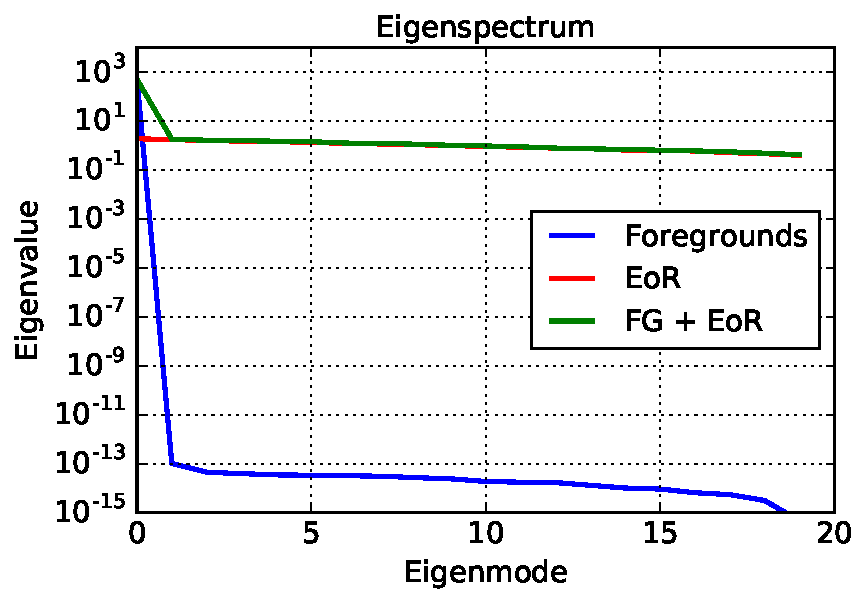
\includegraphics[trim={0cm 0cm 0cm 0cm},clip,width=\columnwidth]{plots/toy_sigloss2.pdf}
	\caption{Eigenspectrum of $\widehat{\textbf{C}}_{\rm FG}$ (blue), $\widehat{\textbf{C}}_{\rm EoR}$ (red), and $\widehat{\textbf{C}}_{\rm FG+EoR}$ 
(green). The eigenspectrum of $\widehat{\textbf{C}}_{\rm FG}$ peaks at the zeroth eigenmode, due to the presence of only one 
sinusoid. These empirically estimated covariance matrices have eigenspectra that are different from that of the true $\textbf{C}$. Specifically, these eigenmodes have the risk of being down-weighted more significantly than they should be because they are coupled to the data in a way that produces loss.}
	\label{fig:toy_sigloss2}
\end{figure}

Because $\widehat{\textbf{C}}$ is estimated from the data, its eigenvectors and eigenvalues are strongly coupled to the particular data realization that was used to compute it. For example, the highest-valued eigenmode of $\widehat{\textbf{C}}$ (highest eigenvalue) describes the sinusoid foreground mode in the toy model (the peak in Figure \ref{fig:toy_sigloss3}). In Figure \ref{fig:toy_sigloss12} we show the estimated covariances of our toy model datasets along with $\widehat{\textbf{C}}^{-1}$ weighted data. The foreground sinusoid is clearly visible in $\widehat{\textbf{C}}_{\rm FG}$.

In general, the highest-valued eigenmodes of $\widehat{\textbf{C}}$ typically (but not always) describe bright foregrounds --- the most prominent shapes in a dataset. For these FG-dominating modes, where foregrounds outshine the EoR signal, down-weighting is beneficial. In some sense, we desire signal loss in this regime, if by `signal' we mean `foregrounds.' In this case it is beneficial for these eigenmodes to be coupled to the data in a way that produces loss. For our toy model, the successful suppression of the foreground mode is demonstrated in Figure \ref{fig:toy_sigloss3} by the missing foreground peak in the weighted power spectrum estimate (green).

%If the true covariance matrix $\textbf{C}$ of our data was known, then every single eigenvalue and eigenvector of $\textbf{C}$ would be 
%representative of real fluctuations in the data. However, when using an estimated $\widehat{\textbf{C}}$ that is derived from one 
%particular data realization, its eigenvalues and eigenvectors may differ from the truth. Said differently, shapes that may not exist (or exist rarely) in a true covariance may appear stronger in the estimated covariance. Hence, they will be down-weighted 
%more than they should be.

\begin{figure}
	\centering
	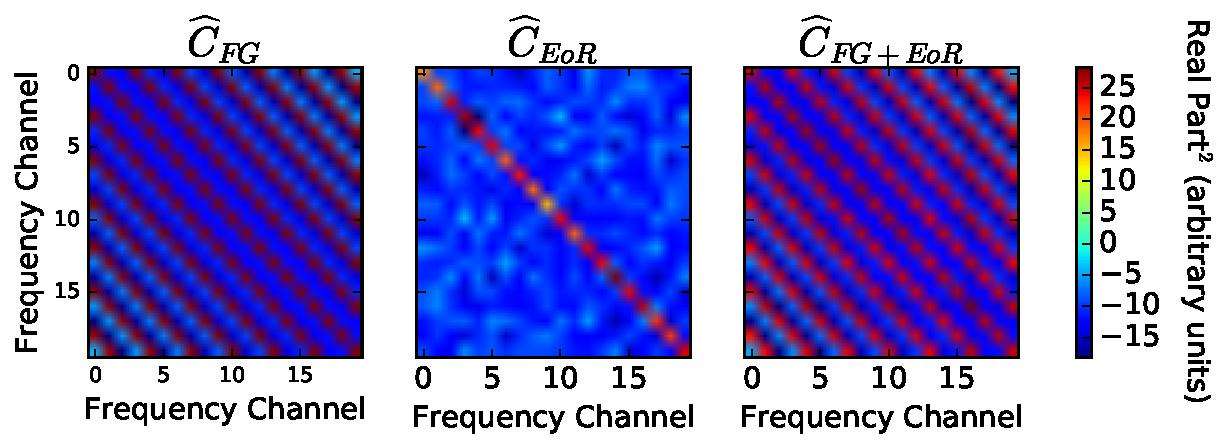
\includegraphics[trim={0cm 0cm 0cm 0cm},clip,width=\columnwidth]{plots/toy_sigloss12.pdf}
	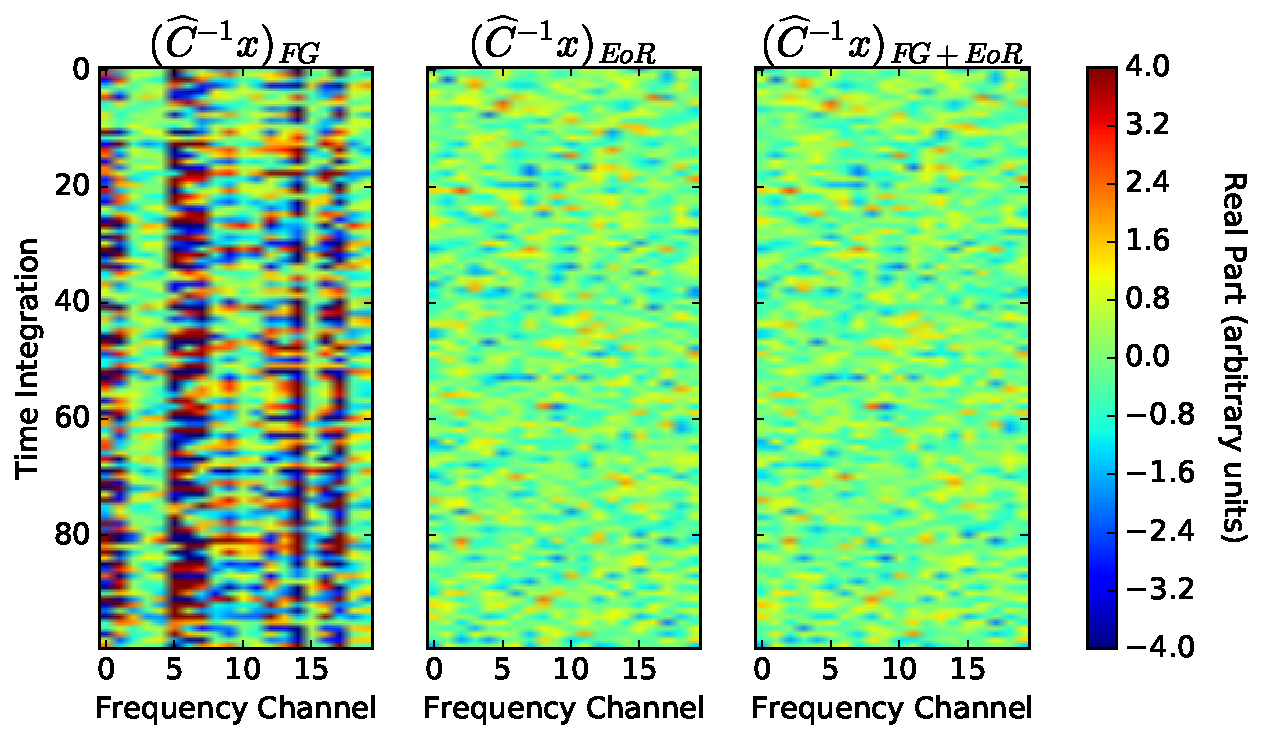
\includegraphics[trim={0cm 0cm 0cm 0cm},clip,width=\columnwidth]{plots/toy_sigloss13.pdf}
	\caption{The estimated covariance matrices (top row) and inverse covariance-weighted data (bottom row) for FG only (left), EoR only 
(middle), and FG + EoR (right). Real parts are shown here.}
	\label{fig:toy_sigloss12}
\end{figure}

The danger of an empirically estimated covariance matrix comes mostly from not being able to describe the EoR-dominating eigenmodes of $
\textbf{C}$ accurately, for which the EoR signal is brighter than foregrounds. In such a case, the coupling between these modes to the data realization leads to the overfitting and subtraction of the EoR signal. More specifically, the coupling between the estimated covariance and the data is anti-correlated in nature (which is explained in more detail in Section \ref{sec:siglossmethod}), which leads to loss. Mis-estimating $\textbf{C}$ for EoR-dominated eigenmodes is therefore more harmful than for FG-dominated modes, and since the lowest-valued eigenmodes of an eigenspectrum are typically EoR-dominated, using this part of the spectrum for weighting is most dangerous.

Using what we've learned about the eigenspectrum, we can tweak it in a simple way to suppress foregrounds and yield minimal 
signal loss. Recall that our toy model foreground is a sinusoid, so it can be perfectly described by a single eigenmode. Using the full dataset's (foreground plus EoR signal) empirical covariance, we can 
project out the first eigenmode and then flatten the rest of the spectrum to have eigenvalues of 1, thereby down-weighting the foreground-dominated mode more than the rest of the modes. Hence, we are changing the EoR-dominating part of the spectrum to be less coupled to the data, limiting the amount of over-fitting that can happen for those modes (i.e. only allowing over-fitting to occur for the first mode).

Altering $\widehat{\textbf{C}}$ as such is one specific example of a regularization method for this toy model, in which we are 
changing $\widehat{\textbf{C}}$ in a way that changes its coupling to the data realization. The resulting 
power spectrum estimate for this case is shown in the right plot of Figure \ref{fig:toy_sigloss3}. In this case we recover the EoR signal, 
demonstrating that if we can disentangle the foreground-dominating modes and EoR-dominating modes, we can down-weight 
them with negligible signal loss. There are several other ways to regularize $\widehat{\textbf{C}}$, and we will discuss some in Section 
\ref{sec:otherweight}.

\subsubsection{Toy Model: Fringe-Rate Filtering}
\label{sec:toymodel_frf}

We have shown how signal loss can arise due to the coupling of EoR-dominated eigenmodes to the data. We will next show how this effect is exacerbated by reducing the total number of independent 
samples in a dataset. 

A fringe-rate filter is an analysis technique designed to maximize sensitivity by integrating in time (\citealt{parsons_et_al2016}). 
Rather than a traditional box-car average in time, a time domain filter can be designed to up-weight temporal modes consistent with 
the sidereal motion on the sky, while down-weighting modes which are noise-like. 

Because fringe-rate filtering is analogous to averaging in time, it comes at the cost of reducing the total number of independent 
samples in the data. To mimic this filter, we average every four time integrations of our toy model dataset together, yielding 
$25$ independent samples in time (Figure \ref{fig:toy_sigloss5}). We choose these numbers so that the total number of 
independent samples is similar to the number of frequency channels --- hence our matrices will still be full rank.
%\footnote{If instead we average every $20$ samples together, yielding only $5$ independent samples in time, we are left with a rank deficient covariance matrix. In this case... \cc{fill in}}

The resulting eigenspectrum as compared to the green curve (FG + EoR) in Figure \ref{fig:toy_sigloss2} is shown in Figure 
\ref{fig:toy_sigloss15}. With 
fringe-rate filtering resulting in fewer independent modes, it becomes more difficult for the empirical covariance to estimate the 
true covariance matrix of the fringe-rate filtered data. This can be quantified by evaluating a convergence metric $\varepsilon(\Chat)$ for the empirical covariance, which we define as
\begin{equation}
\label{eq:converge}
\varepsilon (\Chat) \equiv \sqrt{\frac{\sum_{ij} (\widehat{C}_{ij} - {C}_{ij})^2}{\sum_{ij} {C}_{ij}^2}},
\end{equation}
where $\C$ is the true covariance matrix. To compute this metric, we draw different numbers of realizations (different draws of Gaussian noise) of our toy model EoR measurement, $\textbf{x}_{\rm EoR}$, and take their ensemble average. We then compare this to the ``true' covariance, which in our simulation is set to be the empirical covariance after a large number ($500$) of realizations. As shown in Figure \ref{fig:toy_sigloss16}, we perform this computation for a range of total independent ensemble realizations (horizontal axis) and the number of independent samples in the data following fringe-rate filtering (different colors). With more independent time samples (i.e. more realizations) in the data, one converges to the true fringe-rate filtered covariance more quickly. 

The situation here with using a finite number of time samples to estimate our covariance is analogous to a problem faced in galaxy surveys, where the non-linear covariance 
of the matter power spectrum is estimated using a large --- but finite --- number of expensive simulations. There, the limited 
number of independent simulations results in inaccuracies in estimated covariance matrices 
\citep{dodelson_schneider2013,taylor_joachimi_etal2014}, which in turn result in biases in the final parameter constraints 
\citep{hartlap_et_al2007}. In our case, the empirically estimated covariances are used for estimating the power spectrum, and 
as we discussed in the previous section (and will argue more thoroughly in Section \ref{sec:siglossmethod} and Appendix \ref{sec:sigloss_appendix}), couplings between these covariances and the data can lead to power spectrum estimates that are biased 
\emph{low}---which is precisely signal loss. In future work, it will be fruitful to investigate whether advanced techniques from the 
galaxy survey literature for estimating accurate covariance matrices can be successfully adapted for $21\,\textrm{cm}$ 
cosmology. These techniques include the imposition of sparsity priors \citep{padmanabhan_et_al2016}, the fitting of 
theoretically motivated parametric forms \citep{pearson_samushia2016}, covariance tapering \citep{paz_sanchez2015}, 
marginalization over the true covariance \citep{sellentin_heavens2016}, and shrinkage methods 
\citep{pope_szapudi2008,joachimi_2017}.

Just as important as the eigenvalues are the eigenvectors of our empirical covariances. In general, different eigenvectors converge to their true forms at different rates. This is illustrated by Figure \ref{fig:toy_sigloss17}, which shows the convergence of eigenvectors in an empirical estimate of a covariance matrix whose true form is a diagonal matrix with eigenvalues spanning four orders of magnitude. We use as a convergence metric $\varepsilon(\widehat{\textbf{v}})$ for the empirical eigenvectors $\widehat{\textbf{v}}$, defined as:
\begin{equation}
\label{eq:converge_eig}
\varepsilon (\widehat{\textbf{v}}) \equiv \sqrt{\sum_{i}^{N_{f}}|\textbf{v}-\widehat{\textbf{v}}|_{i}^2},
\end{equation}
where $N_{f}$ is the number of frequencies ($20$) in the mock data. The eigenmode convergence curves  in Figure \ref{fig:toy_sigloss17} are ranked ordered by eigenvalue, such that ``Eigenmode \#0" illustrates the convergence of the eigenvector with the largest eigenvalue, ``Eigenmode \#1" for the second largest eigenvalue, and so on. One sees that the highest-valued eigenmodes converge to their true eigenvectors more quickly. With only a small number of realizations, these empirically estimated modes already retain little correlation with the specific realizations of data that were used to form the empirical covariance. As we will see in the next section, using only these eigenmodes, which are less coupled to data realizations, minimizes signal loss. In contrast, the lower-valued eigenmodes retain more memory of the data realizations, which leads to correlations that induce signal loss. Said differently, a steep covariance eigenspectrum can be especially dangerous because the eigenmodes that converge the slowest are typically also EoR-dominated and are therefore susceptible to the most loss.  %\acl{Think about whether we need to do the Fourier space version as well.}

\begin{figure}
	\centering
	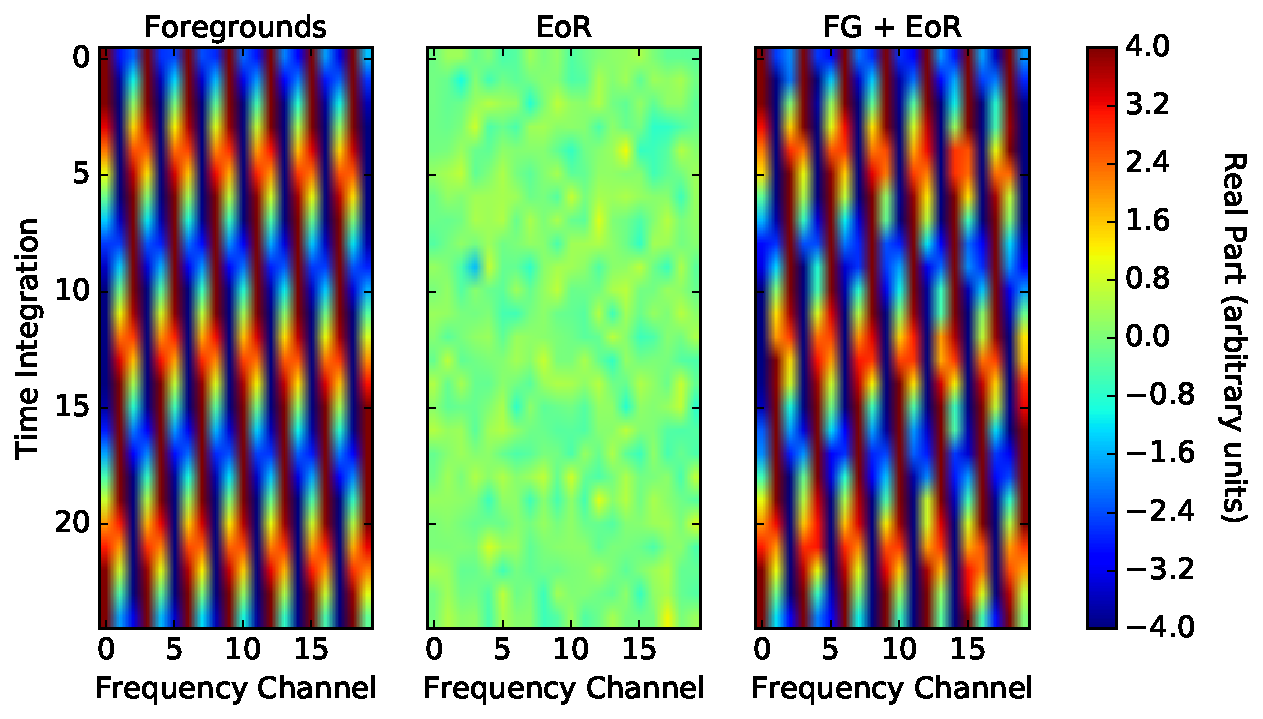
\includegraphics[width=\columnwidth]{plots/toy_sigloss5.pdf}
	\caption{Our `fringe-rate filtered' (time-averaged) toy model dataset. We average every four samples together, 
yielding $25$ independent samples in time. Real parts are shown here.}
	\label{fig:toy_sigloss5}
\end{figure}

\begin{figure}
	\centering
	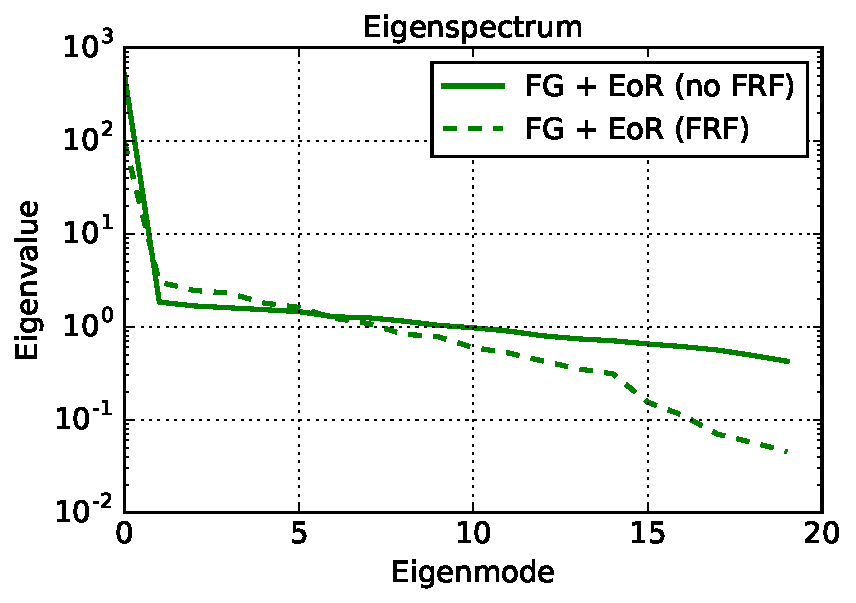
\includegraphics[trim={0cm 0cm 0cm 0cm},clip,height=0.31\textwidth]{plots/toy_sigloss15.pdf}
	\caption{Eigenspectrum of $\widehat{\textbf{C}}_{\rm FG+EoR}$, in the case of no fringe-rate filtering (solid green) and with fringe-rate filtering (dashed green). The dashed, steep eigenspectrum has a greater risk of signal loss because its lowest-valued eigenmodes are both more strongly coupled to the data (than those of the solid eigenspectrum) and, in this example, are also EoR-dominated.}
	\label{fig:toy_sigloss15}
\end{figure}

\begin{figure}
	\centering
	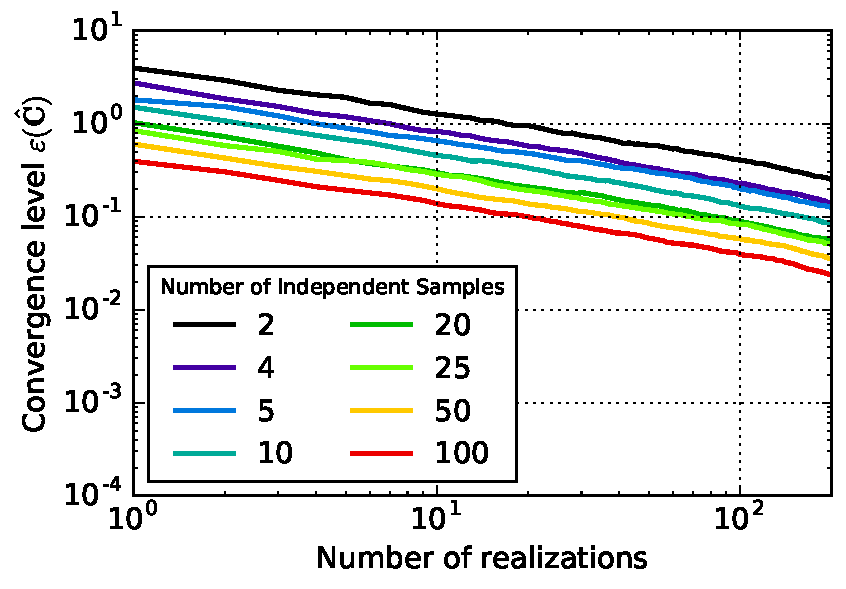
\includegraphics[width=\columnwidth]{plots/toy_sigloss16.pdf}
	\caption{The convergence level, as defined in Equation \eqref{eq:converge}, of empirically estimated covariances of mock EoR signals with different numbers of independent samples. In red, the mock EoR signal is comprised entirely of independent samples. Subsequent colors show time-averaged signals. As the number of realizations increases, we see that the empirical covariances approach the true covariances. With more independent samples, the quicker an empirical covariance converges, and the less signal loss we would expect to result.}
	\label{fig:toy_sigloss16}
\end{figure}

\begin{figure}
	\centering
	\includegraphics[width=\columnwidth]{plots/toy_sigloss17.pdf}
	\caption{The convergence level, as defined in Equation \eqref{eq:converge_eig}, of empirically estimated eigenvectors for different numbers of mock data realizations. The colors span from the 0th eigenmode (has the highest eigenvalue) to the 19th eigenmode (has the lowest eigenvalue), where they are ordered by eigenvalue in descending order. This figure shows that the highest-valued modes converge more quickly than the others, implying that weighting by the lowest-valued empirically estimated modes poses the most risk for loss. Since these modes are also typically EoR-dominated, this can lead to cosmological signal loss.}
	\label{fig:toy_sigloss17}
\end{figure}

\begin{figure}
	\centering
	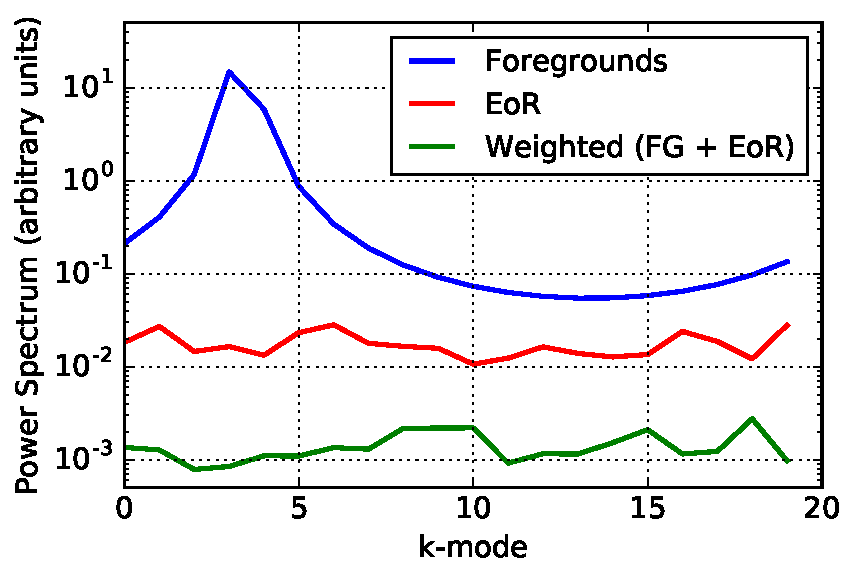
\includegraphics[trim={0cm 0cm 0cm 0cm},clip,width=\columnwidth]{plots/toy_sigloss7.pdf}
	\caption{Resulting power spectrum estimate for the `fringe-rate filtered' (time-averaged) toy model simulation --- foregrounds only (blue), 
EoR only (red), and the weighted FG + EoR dataset (green). We use empirically estimated inverse covariance weighting where $\textbf{C}$ is 
computed from the data. There is a larger amount of signal loss than for the non-averaged data, a consequence of weighting by eigenmodes that are more strongly coupled to the data due to there being fewer independent modes in the data.}
	\label{fig:toy_sigloss7}
\end{figure}


The power spectrum results for the fringe-rate filtered toy model data are shown in Figure \ref{fig:toy_sigloss7}. As 
expected, there is a much larger amount of signal loss for this time-averaged dataset since we do a worse job estimating the true covariance. In addition, as a result of having fewer independent samples, we obtain an estimate with more scatter. This is evident by noticing that the 
green curve in Figure \ref{fig:toy_sigloss7} fails to trace the shape of the uniform-weighted EoR power spectrum.

Using our toy model, we have seen that a sensitivity-driven analysis technique like fringe-rate filtering has trade-offs of signal 
loss and noisier estimates when using data-estimated covariance matrices. Longer integrations increase sensitivity but reduce 
the number of independent samples, resulting in poorly characterized, steep eigenspectra that can overfit signal greatly. We 
note that a fringe-rate filter does have a range of benefits, many described in \citet{parsons_et_al2016}, so it can still be 
advantageous to use one despite the trade-offs.

\subsubsection{Toy Model: Other Weighting Options}
\label{sec:otherweight}

In Section \ref{sec:toymodel} we showed one example of how altering $\widehat{\textbf{C}}$ can 
make the difference between nearly zero and some signal loss. We will now use our toy model to describe several other ways to tailor $\widehat{\textbf{C}}$ 
in order to minimize signal loss. We choose four independent regularization methods to highlight in this section, which have 
been chosen due to their simplicity in implementation and straightforward interpretations. We illustrate the resulting power 
spectra and eigenspectra for the different cases in Figures \ref{fig:toy_sigloss8} and \ref{fig:toy_sigloss14}. These examples are not meant to be taken as suggested analysis methods but rather as illustrative cases. 

As a first test, we model the covariance matrix of EoR as a proof of concept that if perfect models are known, signal loss can be 
avoided. We know that our simulated EoR signal should have a covariance matrix that mimics the identity matrix, with its 
variance encoded along the diagonal. We model $\textbf{C}_{\rm EoR}$ as such (i.e. the identity), instead of computing it based on $\textbf{x}
_{\rm EoR}$ itself. Next, we add $\textbf{C}_{\rm EoR} + \widehat{\textbf{C}}_{\rm FG}$ (where $\widehat{\textbf{C}}_{\rm FG} = \langle\textbf{x}_{\rm FG}
\textbf{x}_{\rm FG}^{\dagger}\rangle_{t}$) to obtain a final $\widehat{\textbf{C}}$ to use in weighting. In Figure \ref{fig:toy_sigloss8} (upper 
left), we see that there is negligible signal loss. This is because by modeling $\textbf{C}_{\rm EoR}$, we avoid over-fitting EoR fluctuations in the data that our model doesn't know about (but an empirically derived $\widehat{\textbf{C}}_{\rm EoR}$ would). This is also shown by comparing the (steeper) green and (flatter) red curves in Figure \ref{fig:toy_sigloss14}. In practice such a weighting option is not feasible, as it is difficult to model $\textbf{C}_{\rm EoR}$, and $\widehat{\textbf{C}}_{\rm FG}$ is unknown because we don't know how to separate out the foregrounds from the EoR in our data.

\begin{figure*}
	\centering
	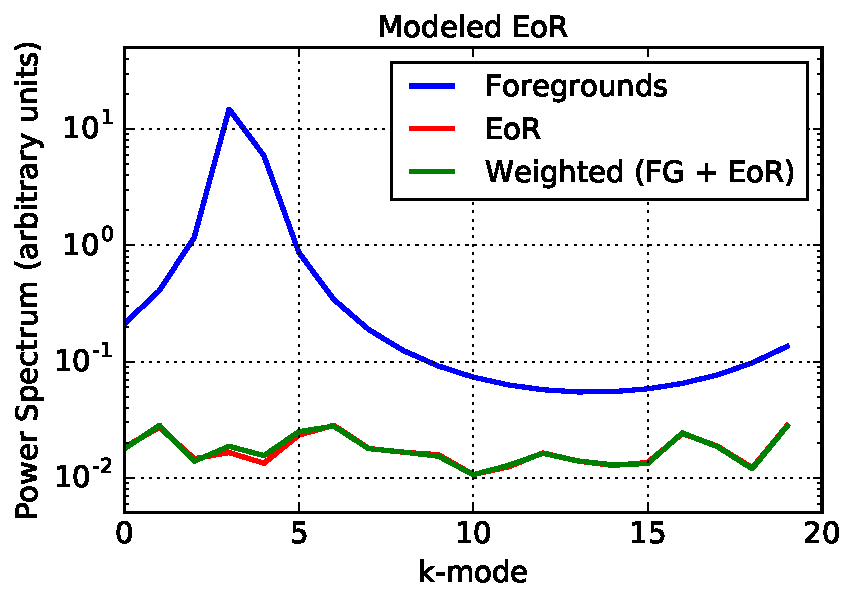
\includegraphics[trim={0cm 0cm 0cm 0cm},clip,height=0.3\textwidth]{plots/toy_sigloss10.pdf}
	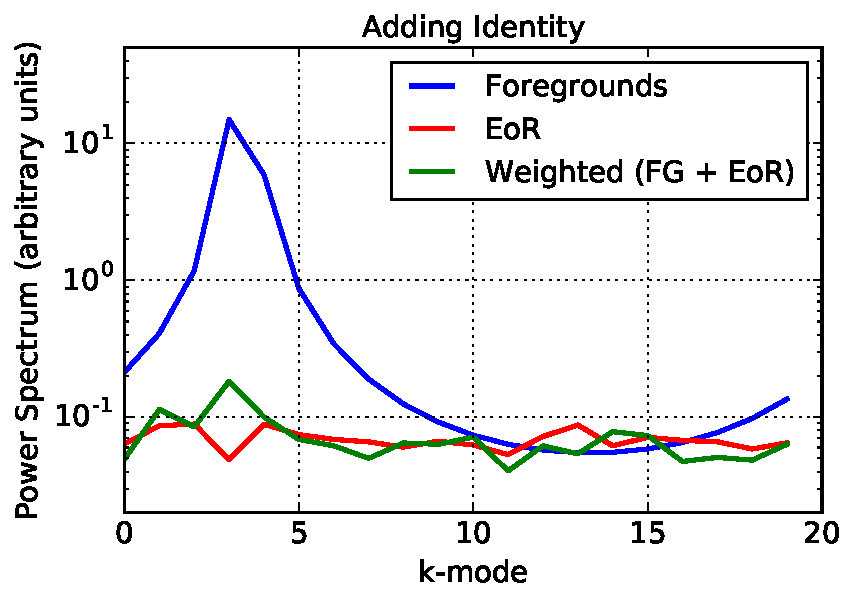
\includegraphics[trim={0cm 0cm 0cm 0cm},clip,height=0.3\textwidth]{plots/toy_sigloss8.pdf}
	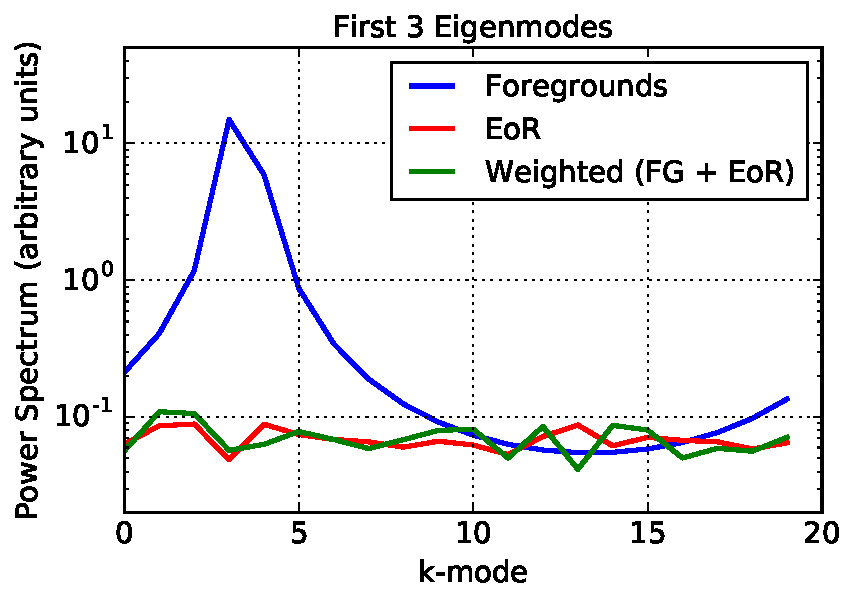
\includegraphics[trim={0cm 0cm 0cm 0cm},clip,height=0.3\textwidth]{plots/toy_sigloss9.pdf}
	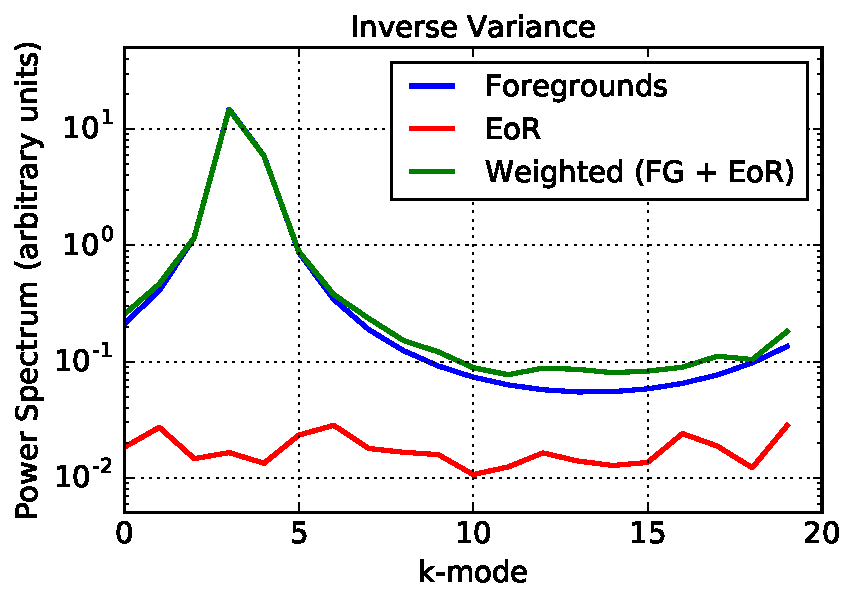
\includegraphics[trim={0cm 0cm 0cm 0cm},clip,height=0.3\textwidth]{plots/toy_sigloss11.pdf}
	\caption{Resulting power spectra estimates for our `fringe-rate filtered' (time-averaged) toy model simulation --- foregrounds only (blue), 
EoR only (red), and the weighted FG + EoR dataset (green). We show four alternate weighting options that each minimize signal 
loss, including modeling the covariance matrix of EoR (upper left), regularizing $\widehat{\textbf{C}}$ by adding an identity matrix to 
it (upper right), using only the first three eigenmodes of $\widehat{\textbf{C}}$ (lower left), and keeping only the diagonal elements of 
$\widehat{\textbf{C}}$ (lower right). The first case (upper left) is not feasible in practice since we do not know $\textbf{C}_{\rm FG}$ and $\textbf{C}_{\rm EoR}$ like we do in the toy model.}
	\label{fig:toy_sigloss8}
\end{figure*}

\begin{figure}
	\centering
	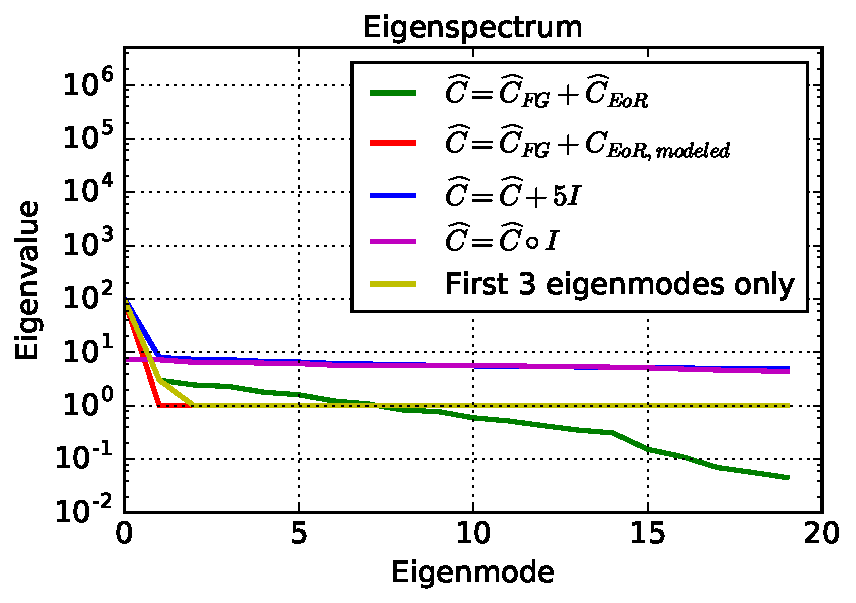
\includegraphics[trim={0cm 0cm 0cm 0cm},clip,width=\columnwidth]{plots/toy_sigloss14.pdf}
	\caption{We compare the eigenspectrum of an empirically calculated $\widehat{\textbf{C}}$ (green) to that of four alternate 
weighting options, including modeling the covariance matrix of EoR (red), regularizing $\widehat{\textbf{C}}$ by adding an identity 
matrix to it (blue), using only the first three eigenmodes of $\widehat{\textbf{C}}$ (yellow), and multiplying an identity matrix with $
\widehat{\textbf{C}}$ (magenta). All eigenspectra (except the green) are relatively flat and don't exhibit signal loss. All were 
computed for the `fringe-rate filtered' (time-averaged) toy model case presented in Section \ref{sec:toymodel_frf}.}
	\label{fig:toy_sigloss14}
\end{figure}

The second panel (top right) in Figure \ref{fig:toy_sigloss8} uses a regularization method of setting $\widehat{\textbf{C}} \equiv 
\widehat{\textbf{C}} + \gamma\textbf{I}$, where $\gamma = 5$ (an arbitrary strength 
of $\textbf{I}$ for the purpose of this toy model). By adding the identity matrix, element-wise, we are weighting the diagonal 
elements of the estimated covariance matrix more heavily than those off-diagonal. Since the identity component does not know anything about the data realization, it alters the covariance to be less coupled to the data. Although there is negligible signal loss using this regularization, the small green peak at the third $k$-mode represents residual foregrounds that still exist since the shapes encoded in the off-diagonal frequency correlations of the covariance matrix were deemed not as prominent as the diagonal elements using this weighting scheme. 

The third panel (bottom left) in Figure \ref{fig:toy_sigloss8} minimizes signal loss a different way --- 
by only using the first three eigenmodes of the estimated covariance. Recalling that our toy model foregrounds can be described entirely by the first eigenmode, this 
method intentionally projects out the highest-valued modes only by replacing all but the three highest weights in the 
eigenspectrum with $1$'s (equal weights). Again, avoiding the over-fitting of EoR-dominating modes which are coupled to the data results in negligible signal loss. However, we do 
not perfectly recover the shape of the EoR power spectrum because we lost information when ignoring the relative weights of most modes. While this case is illuminating for the toy model, in practice it is not obvious which eigenmodes are FG or EoR dominated (and they could be mixed as well), so determining which subset of modes to down-weight is not trivial. 

The last regularization scheme we are highlighting here is setting $\widehat{\textbf{C}} \equiv \widehat{\textbf{C}} \circ \textbf{I}$ (element-wise multiplication), or inverse variance weighting (keeping only the diagonal elements of $\widehat{\textbf{C}}$). In the bottom right 
panel of Figure \ref{fig:toy_sigloss8}, we see that this method does not down-weight the foregrounds --- this regularization altered $\widehat{\textbf{C}}$ in a way where it is no longer coupled to any of the empirically estimated eigenmodes. For this toy model, 
our foregrounds are spread out in frequency and therefore have non-negligible frequency-frequency correlations. Multiplying by 
the identity, element-wise, results in a diagonal matrix, meaning we do not have any correlation information. Because of this, we do a poor job 
suppressing the foreground. But because we de-coupled the whole eigenspectrum from the data, we also avoid signal loss. Although this method did not successfully recover the EoR signal for this particular simulation, it is important that we show that there 
are many options for estimating a covariance matrix, and some may down-weight certain eigenmodes more than others based on the spectral nature 
of the components in a dataset. 
%One may imagine a situation where a particular systematic is contained to an isolated 
%frequency (such as radio frequency interference or crosstalk). In such a case, preserving only the diagonal elements of $
%\widehat{\textbf{C}}$ would be an effective way of removing this contamination. 

In summary, we have a choice of how to weight 21\,cm data. Ideally, we want to down-weight bright foregrounds without 
removing the underlying cosmological signal. However, there are trade-offs between the weighting method 
used, its foreground-removal effectiveness, the number of independent samples in a dataset, and the amount of resulting signal loss. 

% SECTION 2 ERROR ESTIMATION ---------------------------------------------------------------------------------

\subsection{Error Estimation}
\label{sec:ErrorOverview}

Our second major 21\,cm power spectrum theme is error estimation, as we desire robust methods for determining accurate 
confidence intervals for our measurements. Two popular ways of calculating errors on a power spectrum 
measurement are calculating the variance of power spectrum results, and computing a theoretical error estimate based on an instrument's 
system temperature and observational parameters. In a perfect world, both methods would match up. However, in practice the 
two do not always agree due to a number of factors, including possible non-Gaussianities in the noise properties of our instruments and possible systematics in the data.

A third option which acts as a middle ground between purely theoretical and purely empirical errors is using Gaussian error. This involves the assumption of Gaussianity, but allows the variance of the power spectrum estimator to be written as a function of the two-point estimator, or covariance. One could empirically calculate the covariance and then propagate it into an analytic expression to compute the errors, making this method fall somewhere between being fully empirical and fully modeled (see \citet{das_et_al2011a} for an example of its implementation). 

For PAPER's analysis, we choose a data-driven method of error estimation that does not rely on assumptions of Gaussianity. Namely, we compute error bars that have been derived from the inherent 
variance of our measurements. A common technique used to do this is bootstrapping. For pedagogical purposes, we first define the technique of 
bootstrapping and then illustrate one of its pitfalls through a toy model.

Bootstrapping uses sampling with replacement to estimate a posterior distribution. For example, measurements (like power 
spectra) can be made from different samples of data. Each of these measurements is a different realization drawn from some underlying distribution, and realizations are correlated with each other to a degree set by the fraction of sampled points that are held in common 
between them. Through the process of re-sampling and averaging along different axes of a dataset, such as along baselines or times, we can estimate error bars for 
our results which represent the underlying distribution of values that are allowed by our measurements (\citealt{efron_tibshirani1994}; \citealt{andrae2010}).

Suppose we have $N$ different measurements targeting the same quantity (for example, $N$ power spectrum measurements). 
Bootstrapping means that we form $N_{\rm boot}$ (often a large number) bootstraps, where each bootstrap is a random selection 
of the $N$ measurements. Bootstraps each have dimensions of $N$, and the values populated into each bootstrap are drawn 
from the original set of measurements with replacement (i.e. every $n^{th}$ slot in $N$ is filled randomly for each bootstrap). Next we take 
the mean of each bootstrap to collapse it from an array of length $N$ to a single number (we are interested in the mean statistic 
here, but any function of interest can be applied to each bootstrap as long as it's the same function for each one). The error (on 
the mean) is then computed as the standard deviation across all bootstraps. 

We must be careful in distinguishing $N_{\rm boot}$, the number of bootstraps, from $N$, the number of samples, or elements, or 
values, that comprise a bootstrap. In the toy models presented in this section, $N_{\rm boot}$ is typically large, and the standard 
deviation across bootstraps (the error we are computing) converges for large $N_{\rm boot}$. Typically $N$ is a straightforward value to set that just depends on the experiment. However, we will illustrate one case in which it is not simply the number of samples along the axis that is being re-sampled. More specifically, we will see that $N$ depends on sample independence and may not always be straightforward to approximate. 

For our toy model, suppose we have a Gaussian random signal dataset of length $N=1000$ and unity variance (zero mean). 
This could represent $1000$ power spectrum measurements, for which we are interested in its error. We predict that the error 
on the mean should obey $1/\sqrt{N}$, where $N$ is the number of samples.

We next form $500$ bootstraps ($N_{\rm boot} = 500$). To create each bootstrap, we draw $N$ samples, with replacement, of the 
original data, and take the mean over the $N$ samples. The standard deviation over the $500$ bootstraps gives an error 
estimate for our dataset. This error is indicated by the gray star in Figure \ref{fig:toy_error1} and matches our theoretical 
prediction (green).

One major caveat of bootstrapping arises when working with correlated data. If, for example, a dataset has many repeated 
values inside it, this would be reflected in each bootstrap. The same value would be present multiple times within a bootstrap 
and also be present between bootstraps, purely because it has a more likely chance of being drawn if there are repeats of 
itself. Therefore, bootstrapping correlated data results in a smaller variation between bootstraps, and hence, under-estimates 
errors. The use of a fringe-rate filter, which averages data in time to increase sensitivity, is one example which leads to a 
reduction in the number of independent samples, creating a situation in which errors can be under-estimated. We will now show 
this effect using our toy model.

Going back to our toy model, we apply a sliding boxcar average to $10$ samples at a time, thus reducing the number of 
independent data samples to $N/10 = 100$. Bootstrapping this time-averaged noise, using the same method as described 
earlier (drawing $N$=$1000$ elements per bootstrap sample), under-estimates the error by a factor of $\sim3$ (black points in Figure \ref{fig:toy_error1}, at $N$=$1000$). This occurs 
because we are drawing more samples than independent ones available, and thus some samples are repeated multiple times 
in all bootstraps, leading to less variation between the bootstraps. In fact, the error derived from bootstrapping is a strong 
function of the number of elements that are drawn per bootstrap (Figure \ref{fig:toy_error1}, black points), and we can both 
under-estimate the error by drawing too many or over-estimate it by drawing too few. However, since we know that we have $100$ 
independent samples in this toy model, the error associated with drawing $N$=$100$ samples with replacement does match the theoretical prediction 
as expected (the black points cross the green line at $N$=$100$ in Figure \ref{fig:toy_error1}).

This example highlights the importance of understanding how analysis techniques (e.g. fringe-rate filtering) can affect a 
common statistical procedure like bootstrapping. Bootstrapping as a means of estimating power spectrum errors from real 
fringe-rate filtered data requires knowledge of the number of independent samples, which is not always a trivial task. For 
example, computing the effective number of independent samples of fringe-rate filtered data is not as simple as counting the 
number of averages performed. Down-sampling a time-averaged signal is straightforward using a boxcar average, but non-trivial with a more complicated convolution function that has long tails. Hence, we do not recommend bootstrapping unless the 
number of independent samples along the axis that is being re-sampled is well-determined. In Section \ref{sec:Boot}, we explain how we under-estimated errors in the \citetalias{ali_et_al2015} analysis of PAPER and how our bootstrapping procedure has now changed to avoid the over-sampling of correlated data. 

\begin{figure}
	\centering
	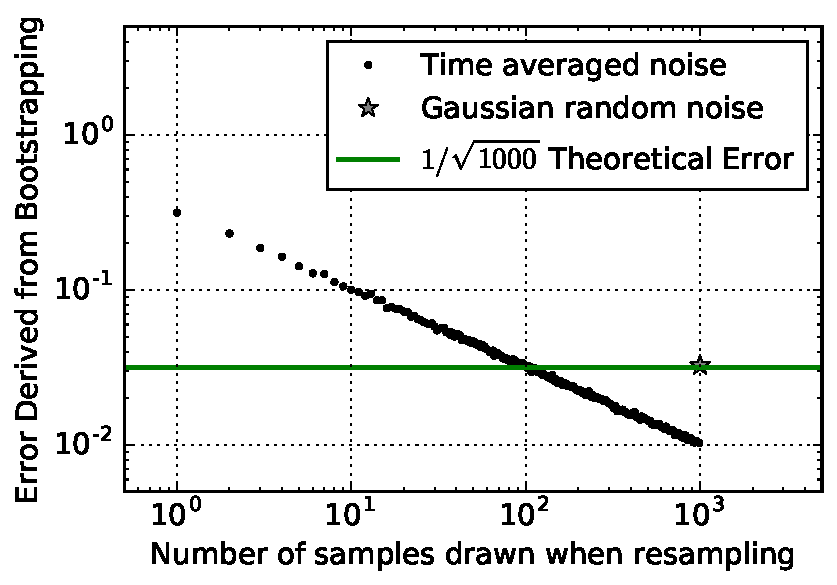
\includegraphics[trim={0cm 0cm 0cm 0cm},width=\columnwidth]{plots/toy_error1.pdf}
	\caption{Error estimation from bootstrapping as a function of the number of elements drawn per bootstrap when 
sampling with replacement. The star represents the standard deviation of $N_{\rm boot}=500$ bootstraps, each created by drawing $1000$ 
elements (with replacement) from a length $1000$ array of a Gaussian random signal. The black points correspond to time-averaged data (correlated data) which has $100$ independent samples. They illustrate how errors can be under-estimated if 
drawing more elements than there are independent samples in the data. The estimated errors match up with the theoretical 
prediction only at $N=100$.}
	\label{fig:toy_error1}
\end{figure}

In summary, bootstrapping can be an effective and straightforward way to estimate errors of a dataset. However, we have 
illustrated a situation in which bootstrapping can lead to under-estimated errors and therefore under-estimated power spectrum limits. We have shown that 
bootstrapped error depends strongly on the number of elements drawn in a bootstrap sample. Estimated errors can drop to 
arbitrarily small values when the number of elements drawn exceeds the effective number of independent elements. 
%We have also shown a situation in which a bootstrapping method does not provide the most sensitive measurement possible. 
While bootstrapping is convenient because it provides a way to estimate errors from the data itself, one must assess whether certain 
analysis choices have compromised the method and whether a variation or an avoidance of traditional re-sampling could be preferred instead.

%\begin{figure}
%	\centering
%	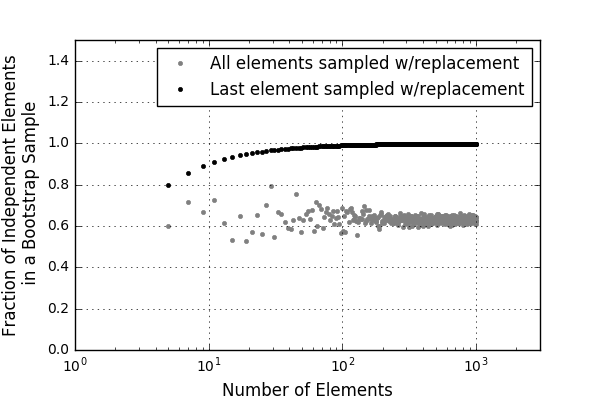
\includegraphics[trim={0cm 0cm 0cm 0cm},width=\columnwidth]{plots/toy_error2.png}
%	\caption{The fraction of independent elements in one bootstrap sample as a function of the total number of elements in a 
%dataset (i.e. if $4$ out of $5$ elements are independent, this would yield a fraction of $0.8$). A fraction of $1.0$ means that all 
%elements in the bootstrap sample are independent, and therefore sensitivity is maximized (alternately, this axis can be thought 
%of as power spectrum sensitivity, where sensitivity increases moving upwards along the y-axis). Two bootstrapping methods are shown here --- sampling all elements with replacement (gray) and sampling only the last element with replacement (black). The former fails to maximize sensitivity since some elements end up being repeated due to random sampling.} 
%The `outlier' points lying at a fraction of $1.0$ at the far left of the plot occur in the off-chance that the last spot in the sample happens to be the one missing element instead of a repeated element --- this is more likely to happen with a small total number of elements but also results in a more dramatically different fraction as compared to the case of a repeated element in the last spot, hence why these points appear like outliers.}
%	\label{fig:toy_error2}
%\end{figure}

% SECTION 2 BIAS ---------------------------------------------------------------------------------

\subsection{Bias}
\label{sec:BiasOverview}

In a 21\,cm power spectrum, detections could be the EoR signal, but they could also 
%(and unfortunately more likely) 
be attributed to other sources of bias. Connecting a detection to EoR as opposed to noise or foreground bias is a key challenge of 
future 21\,cm data analyses \citep[e.g.][]{petrovic_and_oh2011}. In this section we will discuss possible sources of bias in a measurement, as well as techniques 
that can help mitigate their effects. We will also present a series of tests in a pedagogical fashion which we suggest be used to 
help evaluate deep limits and/or detections.

\subsubsection{Foreground and Noise Bias}
\label{sec:BiasTypes}

In Section \ref{sec:SiglossOverview}, we discussed signal loss as a form of multiplicative bias to estimates of the signal. Foregrounds are another type of bias, but an additive instead of a multiplicative one. Foreground bias is perhaps one of the main factors limiting 21\,cm results, as foreground signals lie $\sim4$-$5$ orders of 
magnitude above the cosmological signal. Though there are many techniques proposed for removing foregrounds (see e.g. \citealt{vedantham_et_al2012}; \citealt{chapman_et_al2012}; \citealt{parsons_et_al2012a}; \citealt{parsons_et_al2012b}; \citealt{dillon_et_al2013a}; \citealt{wang_et_al2013}; \citealt{parsons_et_al2014}; \citealt{liu_et_al2014a}; \citealt{wolz_et_al2014}; \citealt{liu_et_al2014b}; \citealt{dillon_et_al2015}; \citealt{pober_et_al2016a}; \citealt{trott_et_al2016}), most 
experiments currently remain limited by residuals rather than noise, especially at low $k$.

One common method to isolate and filter foregrounds is to exploit their behavior in $k$-space. For a particular 
baseline length, there is a maximum delay imposed on sources attached to the sky, which corresponds to the light-crossing time between two 
antennas in a baseline. For longer baselines, this value increases, producing what is known as ``the 
wedge"
\citep{datta_et_al2010, parsons_et_al2012b, vedantham_et_al2012, pober_et_al2013, thyagarajan_et_al2013, liu_et_al2014a, liu_et_al2014b, patil_et_al2017}. 
The wedge describes a region in $k$-space contaminated by smooth spectrum foregrounds, bounded by baseline length (which is proportional to $k_{\perp}$) and delay (which is 
proportional to $k_{\parallel}$). Properties of the wedge can be used to isolate and 
%remove 
avoid foregrounds, as done by \citetalias{ali_et_al2015}, 
\citet{parsons_et_al2014}, \citet{dillon_et_al2014}, \citet{dillon_et_al2015}, \citet{jacobs_et_al2015}, \citet{beardsley_et_al2016}, and \citet{trott_et_al2016}.

Although smooth-spectrum foregrounds preferentially show up at low delay, or low $k$-modes, their isolation within the wedge is not perfect. In deep measurements, power spectrum measurements at $k_{\parallel}$ values beyond 
the delay associated with the length of a baseline are often still contaminated at a low level. This leakage, particularly at low $k$'s, can be attributed to 
convolution kernels associated with Fourier-transforming visibilities into delay-space. In other words, smooth-spectrum 
foregrounds appear as $\delta$-functions in delay-space, convolved by the Fourier transform of the source spectrum, the signal chain, and the 
antenna response, all of which could smear out the foregrounds and cause leakage outside the wedge \citep[e.g.][]{ewall-wice_et_al2017, kerrigan_et_al2018}.

There are analysis techniques to mitigate the effects of foreground leakage and prevent information from low $k's$ from 
spreading to high $k$ values. For example, narrow window functions in delay-space can be used to minimize the leakage from a particular 
$k$ value into other ones (\citealt{liu_et_al2014b}). In other words, one can construct an estimator using QE that forces a 
window function to have a minimum response to low $k$ values. The window function used in \citetalias{ali_et_al2015} is constructed in such a way, 
specifically to prevent foregrounds that live at low $k's$ from contaminating higher $k$-modes (see Section \ref{sec:Bias}). 

Determining the source of positive non-EoR detections at higher $k$'s is more difficult. In previous power spectrum results, these detections have been explained as instrumental systematics, particularly time-variable cross talk, RFI, cable reflections, and calibration errors (\citetalias{ali_et_al2015}; \citealt{parsons_et_al2014}; \citealt{dillon_et_al2014}; \citealt{beardsley_et_al2016}; \citealt{patil_et_al2017}). In the next section, we will present some tests that can help distinguish these excesses from that of EoR. 

In addition to foreground bias, noise can also be responsible for positive power spectrum detections if thermal noise is 
multiplied by itself. Every 21\,cm visibility measurement contains thermal noise that is comprised of receiver and sky noise. 
We expect this noise to be independent between antennas and thus we can beat it down (increase sensitivity) by integrating 
longer, using more baselines, etc. However, the squaring of noise can occur when cross-multiplying visibilities, which is shown by 
the two copies of $\textbf{x}$ in Equation \eqref{eq:qhat}. If both copies of $\textbf{x}$ come from the same baseline and time, it 
can result in power spectrum measurements that are higher than those predicted by the thermal noise of the instrument. One 
way to avoid this type of noise bias is to avoid cross-multiplying data from the same baselines or days. This ensures that the 
two quantities that go into a measurement have separate noises that don't correlate with each other. We also note that if the noise level is known, this type of bias can be subtracted off, though this procedure is argued to be dangerous (\citealt{dillon_et_al2014}; \citealt{parsons_et_al2014}).

Another type of noise bias can stem from the spurious cross-coupling of signals between antennas. This excess is known as 
instrumental crosstalk and is an inadvertent correlation between two independent measurements via a coupled signal path. 
Crosstalk appears as a constant phase bias in time in visibilities, and it varies slowly compared to the typical fringe-rates of 
sources. Because it is slow-varying, crosstalk can be suppressed using time-averages or fringe-rate filters. However, there 
remains a possibility that power spectrum detections that aren't the cosmological signal are caused by residual, low-level crosstalk which survived any 
suppression techniques. 

\subsubsection{Jackknife Tests}
\label{sec:JackknifeOverview}

We now approach the difficult task of tracing excesses to foreground, noise, and EoR biases through a discussion of useful 
jackknife tests. Again, we first approach this topic pedagogically as an introduction to the related PAPER discussion in Section 
\ref{sec:Bias}. 

The jackknife is a resampling technique in which a statistic (i.e. power spectrum) is computed in subsets of the data (\citealt{quenouille1949}; \citealt{tukey1958}). These 
subsets are then compared to reveal systematics. In this section we define two main tests --- the null test and the traditional 
jackknife --- and explain how a power spectrum detection must pass each. We then highlight how these tests can be used to 
help distinguish between different sources of bias.
 
\begin{itemize}
\item \textbf{Null Test}: A null test is a type of jackknife test that removes the astronomical signal from data in order to 
investigate underlying systematics (e.g., see \citet{keating_et_al2016} for examples from intensity mapping that are closely related to our current application). For example, one can 
divide data into two subsets by separating odd and even Julian dates, or the first half of the observing season from the second. 
Subtracting the two removes signal that is common to both subsets, including foregrounds and the EoR signal. The resulting power 
spectrum should be consistent with thermal noise estimates; if it is not, it suggests the presence of a systematic that differs 
from one of the data subsets to the other (i.e. doesn't get subtracted perfectly). 
\item \textbf{Traditional Jackknife}: In a broader sense, it is important to perform many jackknife tests in order to instill 
confidence in a final result. A stable result must be steadfast throughout all jackknives no matter how the data is sliced. 
Jackknives can be taken along several different axes --- for example, one could start with a full dataset, and compute a new 
power spectrum every time as a day of data is removed, or a baseline is removed. This type of jackknife would reveal bias 
present only at certain LSTs (such as a foreground source), for example, or misbehaving baselines.
\end{itemize}

While the null test hunts for deviations from thermal noise and the jackknife tests for deviations in subsamples, they are both 
closely related. We can highlight the connection between the two using a toy model dataset.

Suppose we have four independent measurements made along two different axes. As an example, we construct $\textbf{x}_{1a}$, $\textbf{x}_{1b}$, $\textbf{x}_{2a}$, and $\textbf{x}_{2b}$, where the numbers symbolize two different days of data and the letters represent two different baselines. Each of the 
measurements have dimensions of $100$ time integrations and $20$ frequency channels. They each have separate thermal 
noises constructed as a Gaussian random signal for each, and identical EoR signals. 

To mimic the presence of a systematic, we add a toy sinusoid foreground, similar to the one used in 
Section \ref{sec:toymodel}, to only $\textbf{x}_{2a}$ and $\textbf{x}_{2b}$. This represents a foreground signal 
present in only the second day of data, but not the first. Mathematically, if  $\textbf{n}$ 
is noise, $\textbf{e}$ is the EoR signal, and $\textbf{f}$ is the foreground signal, the four measurements can be written as:

\begin{eqnarray}
\label{eq:bias1}
\textbf{x}_{1a} &=& \textbf{n}_{1a} + \textbf{e}  \\ 
\textbf{x}_{1b} &=& \textbf{n}_{1b} + \textbf{e}  \\ 
\textbf{x}_{2a} &=& \textbf{n}_{2a} + \textbf{e} + \textbf{f} \\ 
\textbf{x}_{2b} &=& \textbf{n}_{2b} + \textbf{e} + \textbf{f}.
\end{eqnarray} 

\noindent We now take a jackknife along the day-axis, forming separate power spectrum estimates for each day:

\begin{eqnarray}
\widehat{\textbf{P}}_{1} &\propto& \textbf{x}_{1a}\textbf{x}_{1b}^{\dagger} \\
\widehat{\textbf{P}}_{2} &\propto& \textbf{x}_{2a}\textbf{x}_{2b}^{\dagger}.
\end{eqnarray}

We do not perform a time-average or apply a fringe-rate filter to this toy model, since we are interested only in what jackknife 
tests can tell us about biases. For the same reason, we use a weighting matrix of $\textbf{I}$ for power spectrum estimation to 
avoid signal loss. 

To construct a null test, we difference the two power spectra, with the result shown in Figure \ref{fig:toy_bias1} (black) along with the power spectrum of noise only (green). Subtracting the two estimates removes sky signal that should ideally be present in both jackknives. However, we see a clear difference between the null test and the power spectrum of 
noise. This signifies a non-EoR bias that is only present in either $\textbf{x}_{1}$ or $\textbf{x}_{2}$, but not both.

\begin{figure}
	\centering
	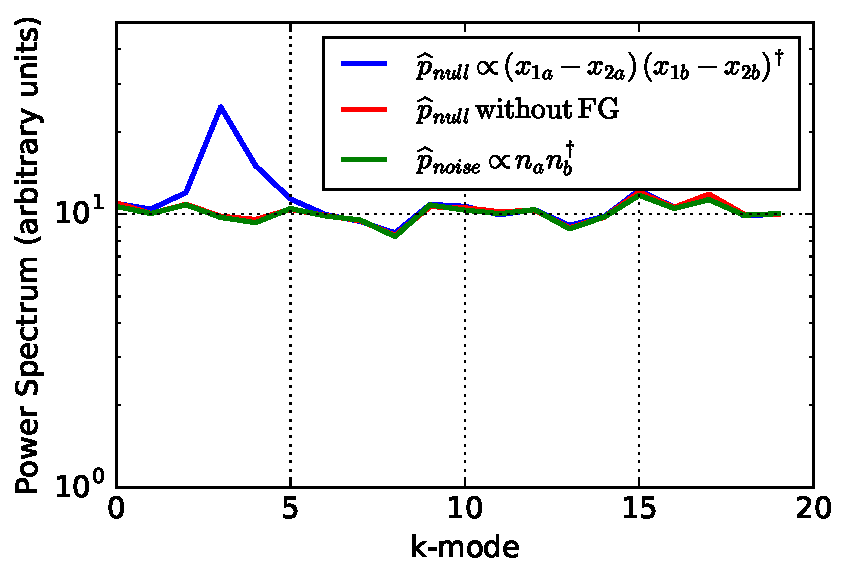
\includegraphics[trim={0cm 0cm 0cm 0cm},width=\columnwidth]{plots/toy_bias1.pdf}
	\caption{A null jackknife test shown as the power spectrum difference between two measurements (black), compared to the power spectrum of noise alone (green). Because the null test is not consistent with noise, it suggests the 
presence of a systematic in either $\textbf{x}_{1}$ or $\textbf{x}_{2}$. Null tests of clean measurements should be consistent 
with thermal noise.}
	\label{fig:toy_bias1}
\end{figure}

\begin{figure}
	\centering
	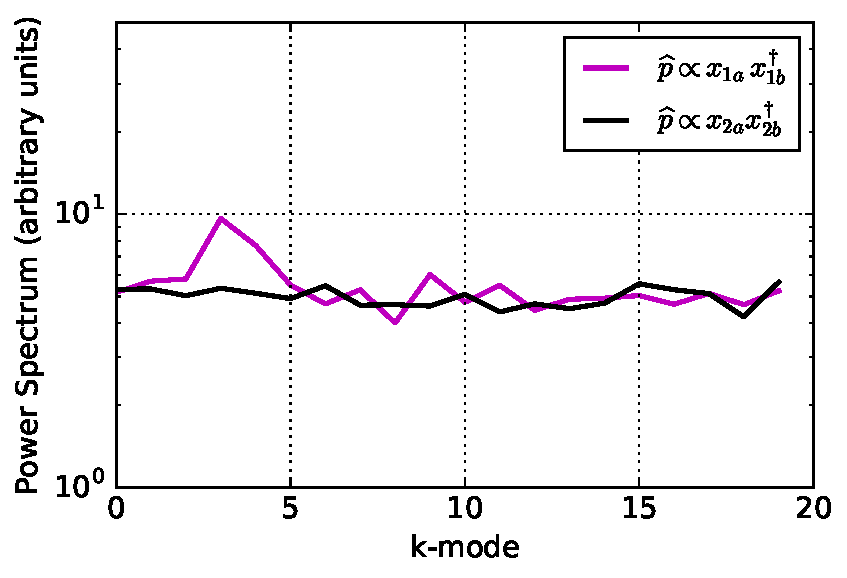
\includegraphics[trim={0cm 0cm 0cm 0cm},width=\columnwidth]{plots/toy_bias2.pdf}
	\caption{Power spectrum estimates for $\textbf{x}_{1}$ and $\textbf{x}_{2}$, two jackknives of the toy model. They suggest 
the presence of a systematic in $\textbf{x}_{2}$ only (which is exactly what was put in), illustrating how jackknives can be used to tease out excesses. Clean 
measurements should remain consistent despite the jackknife taken.}
	\label{fig:toy_bias2}
\end{figure}

While the null test is useful for testing noise properties and the uniformity of a dataset, jackknives are useful in pinpointing 
which data subsets are contaminated by biases and which are not; in our toy model we see that the bias exists only in $
\textbf{x}_{2}$ (Figure \ref{fig:toy_bias2}). If foreground or noise biases exist in a dataset, jackknives can tease them out and 
provide insight into possible sources. For example, if jackknives along the time-axis reveal a bias present at a certain LST, a 
likely explanation would be excess foreground emission from a radio source in the sky at that time. A jackknife test involving 
data before and after the application of a fringe-rate filter can reveal whether crosstalk noise bias is successfully suppressed 
with the filter, or if similar-shaped detections in both power spectra suggest otherwise. There are many other jackknife axes of 
which we will not go into detail here, including baseline, frequency, and polarization. Ultimately, an EoR detection should persist 
through them all and a clean measurement should exhibit noise-like null spectra.

In this section we have highlighted how null tests and jackknife tests are key for determining the nature of a power spectrum 
detection. In Section \ref{sec:Bias} we perform some examples of these tests on PAPER-64 data in order to prove that our 
excesses are not EoR and to identify their likely cause. 

% SECTION 3  ---------------------------------------------------------------------------------

\section{Demonstration in PAPER-64 Data}
\label{sec:CaseStudy}

In the previous sections we have discussed three overarching 21\,cm power spectrum themes --- signal loss, error estimation, 
and bias. Understanding the subtleties and trade-offs involved in each is necessary for an accurate and robust understanding of 
a power spectrum result. 

We now apply these lessons to data from the PAPER experiment, using a subset of the PAPER-64 dataset from
\citetalias{ali_et_al2015}) in order to illustrate our revised analysis pipeline.

As a brief review, PAPER is a dedicated 21\,cm experiment located in the Karoo Desert in South Africa. The PAPER-64 
configuration consists of 64 dual-polarization drift-scan elements that are arranged in a grid layout. For our case study, we 
focus solely on Stokes I estimated data \citep{moore_et_al2013} from PAPER's $30$ m East/West baselines (Figure 
\ref{fig:ant_layout}). All data is compressed, calibrated (using self-calibration and redundant calibration), delay-filtered (to remove foregrounds inside the wedge), LST-binned, and fringe-rate filtered. For detailed information about the backend system of PAPER-64, its observations, and data reduction pipeline, we 
refer the reader to \citet{parsons_et_al2010} and \citetalias{ali_et_al2015}. We note that all data processing steps are identical to those in \citetalias{ali_et_al2015} until after the LST-binning step in Figure 3 of \citetalias{ali_et_al2015}.

\begin{figure}
	\centering
	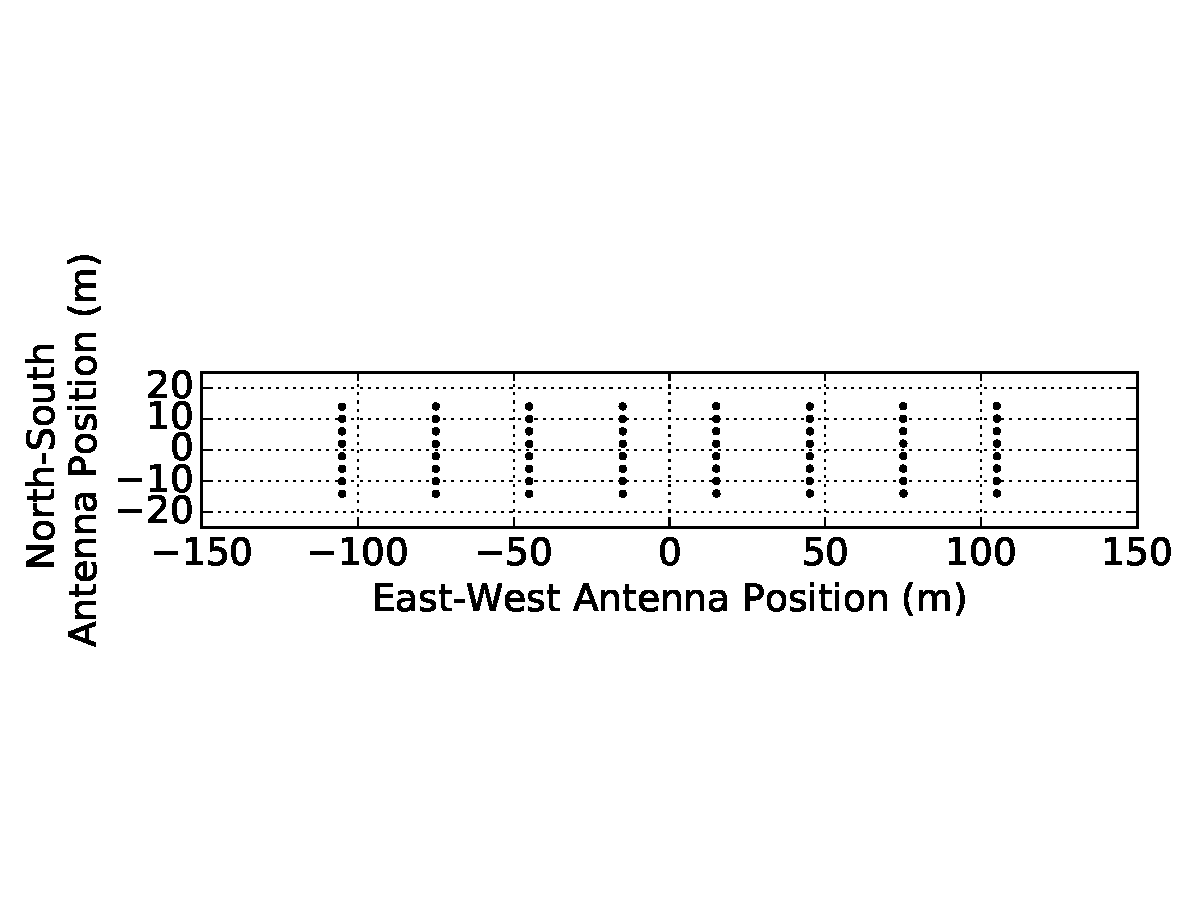
\includegraphics[trim={0cm 3cm 0cm 3cm},width=\columnwidth]{plots/ant_layout_aspect.pdf}
	\caption{The PAPER-64 antenna layout. We use only $10$ of the $30$ m East/West baselines for the analysis in this 
paper (i.e. a subset of the shortest horizontal spacings).}
	\label{fig:ant_layout}
\end{figure}

The previously best published 21\,cm upper limit result from \citetalias{ali_et_al2015} uses $124$ nights of data to place a $2\sigma$ upper limit 
on $\Delta^{2}(k)$, defined as

\begin{equation}
\Delta^{\textbf{2}}(k) = \frac{k^{3}}{2\pi^{2}}\,\hat{P}(k),
\end{equation}

\noindent of $(22.4$ mK$)^{2}$ in the range $0.15 < k < 0.5$\,$h$ Mpc$^{-1}$ at $z = 8.4$. The revision of this limit (Kolopanis et al. (\textit{submitted})) stems from previously under-estimated signal loss and under-estimated error bars, both of which we 
address in the following sections. 

For the analysis in this paper, we use $8.1$ hours of LST, namely an RA range of $0.5$-$8.6$ hours (\citetalias{ali_et_al2015} uses a slightly longer RA 
range of $0$-$8.6$ hours; we found that some early LSTs were more severely foreground contaminated). We also use only $10$ baselines, a subset of the $51$ total East/West baselines used in \citetalias{ali_et_al2015}. All power spectrum results are produced for a center frequency of 151\,MHz using a width of 10\,MHz ($20$ channels), identical to the analysis in \citetalias{ali_et_al2015}. In the case study in this paper, we only use one baseline type instead of the three as in 
\citetalias{ali_et_al2015}, but Kolopanis et al. (\textit{submitted}) uses all baselines presented in \citetalias{ali_et_al2015}.

The most significant changes from \citetalias{ali_et_al2015} occur in our revised power spectrum analysis, which is explained in the rest of this paper, but we also note that the applied fringe-rate filter is also slightly different. In \citetalias{ali_et_al2015}, the 
applied filter was not equivalent to the optimal fringe-rate filter (which is designed to maximize power spectrum sensitivity). Instead, the optimal filter was degraded by widening it in fringe-rate space. This was chosen in order to increase the number of independent 
modes and reduce signal loss, though as we will explain in the next section, this signal loss was still under-estimated. With the development of a new, 
robust method for assessing signal loss, we choose to use the optimal filter in order to maximize sensitivity. This filter is 
computed for a fiducial 30\,m baseline at 150\,MHz, the center frequency in our band. The filter in both the fringe-rate 
domain and time domain is shown in Figure \ref{fig:frp}.

\begin{figure}
	\centering
	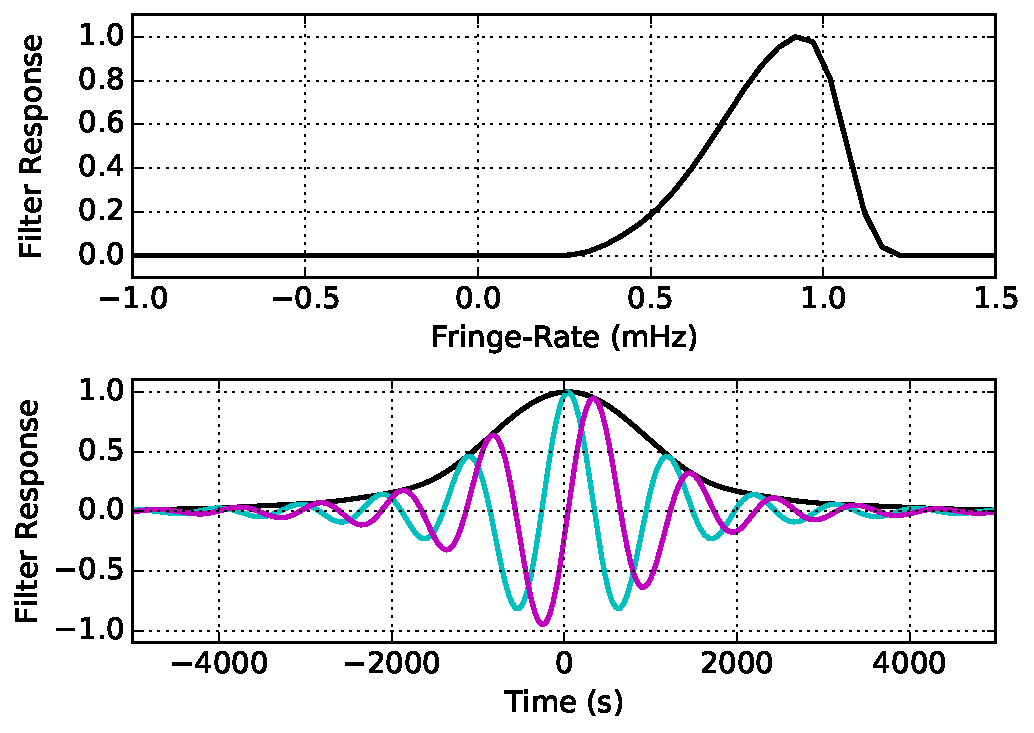
\includegraphics[width=\columnwidth]{plots/frp.pdf}
	\caption{Top: the normalized optimal power-spectrum sensitivity weighting in fringe-rate space for our fiducial baseline and 
Stokes I polarization beam. Bottom: the time-domain convolution kernel corresponding to the top panel. Real and imaginary 
components are illustrated in cyan and magenta, respectively, with the absolute amplitude in black. The fringe-rate filter acts as 
an integration in time, increasing sensitivity but reducing the number of independent samples in the dataset.}
	\label{fig:frp}
\end{figure}

% SECTION 3 SIGNAL LOSS ---------------------------------------------------------------------------------

\subsection{PAPER-64: Signal Loss}
\label{sec:Sigloss}

In Section \ref{sec:SiglossOverview}, we showed how signal loss arises when weighting data using information from the data itself. Here we describe a methodology for estimating the amount of signal loss caused by a particular power spectrum estimator when applied to a particular dataset. The exact amount of signal loss will depend on the specific realizations of the signals present in the data and is not something we can directly compute. In this work, as in \citetalias{ali_et_al2015}, we inject simulated cosmological signals into our data and test the recovery of those signals (an approach also taken by \citet{masui_et_al2013}). As we will see, correlations between the injected signals and the data are significant complicating factors which were previously not taken into account. 

We present our PAPER-64 signal loss investigation in three parts: we first give an overview of our injection framework and illustrate how different power spectrum components affect loss. We next describe our methodology in practice and detail how we map our simulations into a posterior for the EoR signal. Finally, we build off of Section \ref{sec:SiglossOverview} by experimenting with different regularization schemes on PAPER data in order to minimize loss. Throughout each section, we also highlight major differences from the signal loss computation used in \citetalias{ali_et_al2015}, which previously under-estimated losses.

%The results of such an injection scheme can be interpreted in multiple ways. In this paper we describe two --- this section describes one and in Appendix \ref{sec:Pr_appendix} we present an alternate interpretation. These two methods yield very similar results, but fundamentally are answering subtly distinct questions. We also highlight major differences from the signal loss computation used in \citetalias{ali_et_al2015}, which previously underestimated losses. 

\subsubsection{Signal Loss Methodology} 
\label{sec:siglossmethod}
In short, our method consists of adding an EoR-like signal into the data and then measuring how much of this injected signal would be detectable given any attenuation of this signal by the (lossy) data analysis pipeline.  To capture the full statistical likelihood of signal loss, one requires a quick way to generate many realizations of simulated 21\,cm signal visibilities. Here we use the same method as in \citetalias{ali_et_al2015}, where mock Gaussian noise visibilities (mock EoR signals) 
are filtered in time using an optimal fringe-rate filter to retain only ``sky-like" modes. Since the optimal filter has a shape that matches the rate of the sidereal motion of the sky, this transforms the Gaussian noise into a measurement that PAPER could make. This signal is then added to the data.\footnote{One 
specific change from \citetalias{ali_et_al2015} is that we add this simulated signal into the analysis pipeline before the final fringe-rate filter is 
applied to the data. Previously, the addition was done after that final fringe-rate filter step.  This change results in an increased 
estimate of signal loss, %(by a factor of $\sim$$10$), 
likely due to the use of the fringe-rate filter as a simulator. However, this pipeline difference, while significant, is not the dominant reason why signal loss was under-estimated in \citetalias{ali_et_al2015} (the dominant reason is explained in the main text in Section \ref{sec:siglossmethod}).}

Suppose that $\textbf{e}$ is the mock injected EoR signal (at some amplitude level), and $\textbf{x}$ is our data. We define $\textbf{r}
$ to be the data plus the EoR signal:

\begin{equation}
\label{eq:rxe}
\textbf{r} = \textbf{x} + \textbf{e}.
\end{equation}

We are interested in quantifying how much variance in $\textbf{e}$ is lost after weighting $\textbf{r}$ and estimating the power 
spectrum according to QE formalism. We investigate this by comparing two quantities we call the input power spectrum and 
output power spectrum: $\widehat{P}_{\rm in}$ and $\widehat{P}_{\rm out}$, estimated using QE as

\begin{equation}
\label{eq:Pin}
\widehat{P}_{\rm in,\alpha} \equiv \text{M}^{\alpha}_{\rm in}\textbf{e}^{\dagger}\textbf{I}\textbf{Q}^{\alpha}\textbf{I}\textbf{e}
\end{equation}

\noindent and

\begin{eqnarray}
\label{eq:sigloss}
\widehat{P}_{\rm out,\alpha} &\equiv& \widehat{\textbf{P}}_{r,\alpha} \nonumber\\%-\widehat{\textbf{P}}_{x,\alpha} \nonumber \\
&=& \text{M}^{\alpha}_{r}\textbf{r}^{\dagger}\textbf{R}_{r}\textbf{Q}^{\alpha}\textbf{R}_{r}\textbf{r},% - \text{M}^{\alpha}_{x}\textbf{x}^{\dagger}\textbf{R}_{x}\textbf{Q}^{\alpha}\textbf{R}_{x}\textbf{x},
\end{eqnarray}
where, for illustrative purposes and notational simplicity, we have written these equations with scalar normalizations M, even though for our numerical results we choose a non-diagonal matrix normalization using $\mathbf{M}$ as in Equation \eqref{eq:phat}.

The quantity $\widehat{P}_{\rm in}$, defined by Equation \eqref{eq:Pin}, is a uniformly weighted estimator of the power spectrum of $\mathbf{e}$. Since there is no noise contribution to $\mathbf{e}$, it can be considered the power spectrum of this particular realization of the EoR; alternatively, it can be viewed as the true power spectrum of the injected signal up to cosmic variance fluctuations. The role of $\widehat{P}_{\rm in}$ in our analysis is to serve as a reference for the power spectrum that would be measured if there were no signal loss or other systematics. This is then to be compared to $\widehat{P}_{\rm out}$, which approximates the (lossy) power spectrum estimate that is output by our analysis pipeline prior to any signal loss adjustments. In principle, one could compute the true $\widehat{P}_{\rm out}$ using end-to-end simulations of the instrument and data analysis pipeline. In practice, however, such simulations may not accurately reflect real-life systematics and foregrounds. To overcome this obstacle, one can make the assumption that since the EoR signal is expected to be small, the data vector $\mathbf{x}$ itself is our best model of these contaminants. Making this assumption, the injected EoR signal $\mathbf{e}$ takes on the role of the true EoR signal, and the sum of $\mathbf{x}$ and $\mathbf{e}$ (i.e., Equation \eqref{eq:rxe}) replaces $\mathbf{x}$ as our model of the measured data. Therefore, $\widehat{P}_{\rm out}$ can be directly compared to the measurement that we make.

%In the limit where no significant cross-correlations between the data and the injected signals are found, this will recover the amount of injected power spectrum remaining after the covariance weighting operation (i.e. the amount of background EoR power, $P_{\rm eor}$, not removed by the foreground down-weighting procedure). In other words, we make the anzatz that 

%\begin{equation}
%\widehat{P}_{\rm out} = \widehat{\textbf{P}}_{x} \label{eqn:anzatz},
%\end{equation}
%and folding in our definition from Equation \eqref{eq:sigloss}, this ansatz implies that we are seeking the injected 
%signal amplitude which causes a power doubling ($\phat_r = 2 \phat_x$). \cc{I am unsure of this power doubling thing} 

Under this injection framework, we can begin to see explicitly why there can be large signal loss. Expanding out Equation \eqref{eq:sigloss}, $\widehat{P}_{\rm out}$ becomes:

%
%In short, we can approximate a signal loss estimate as the ratio of $\widehat{P}_{\rm out}/P_{\rm in}$, evaluated at the data level $\widehat{\textbf{P}}_{x}$. We motivate the fact that we can evaluate the output-to-input power spectrum ratio at $\widehat{\textbf{P}}_{x}$ by the following reasoning (and then detail our signal loss estimation in practice in the sections that follow).
%
%In the limit of no instrumental noise, the data that we measure, $\x$, is comprised of two signals, such that
%\begin{equation}
%\x \equiv \f + \s,
%\end{equation}
%where $\mathbf{f}$ represents the foregrounds and $\mathbf{s}$ represents the cosmological signal. In general, suppose that our power spectrum algorithm passes the data through some function $g$, yielding a lossy estimate of the power spectrum $\phat_{x}$. This can be parametrized as
%\begin{equation}
%\label{eq:LinearPspecSum}
%\langle \phat_{x} \rangle  = \langle g(\x) \rangle = \ell_{\rm fg} \p_{\rm fg} + \ell_{\rm eor} \p_{\rm eor},
%\end{equation}
%where $\ell_{\rm eor}$ and $\ell_{\rm fg}$ are multiplicative factors accounting for the signal loss in the true EoR 
%power spectrum $\p_{\rm eor}$ and true foreground power spectrum $\p_{\rm fg}$, respectively. It is not 
%\emph{a priori} obvious why this parameterization is suitable; we thus provide a toy model in Appendix 
%\ref{sec:sigloss_appendix} to motivate this, although it should be noted that the derivation is an approximation 
%which assumes that the covariance used in the QE analysis is close to the true covariance with effects due to 
%small sample size limited to first order perturbations and thus neglects cross-correlation between $x$ and $e$.  
%In actual fact the sample size is similar to the number of independent modes, a case were one expects cross 
%terms to be remain significant.   
%
%Given this form, a suitable estimate for $\p_{\rm eor}$ would be $\phat_{x} / \ell_{\rm eor}$, or the uncorrected power spectrum of data divided by the signal loss estimate. Although such an estimate leaves an additive bias from foregrounds (see Section \ref{sec:BiasTypes}) that must be mitigated by other methods (as is the case for any attempt to measure the $21\,\textrm{cm}$ power spectrum), it normalizes $\p_{\rm eor}$ back to its correct level such that there is no multiplicative bias. The most conceptually straightforward way to compute $\ell_{\rm eor}$ is to model the foregrounds and EoR signal via simulations, and then to form the quantity
%\begin{equation}
%\label{eq:Deriv1}
%\widehat{\ell}_{\rm eor} = \frac{g(\f + \s) - g(\f)}{\p_{\rm eor}}.
%\end{equation}
%However, this approach assumes that we have sufficiently good knowledge of our foreground and signal models, which is certainly not the case --- if it were, it would be simpler to construct our covariance matrices from our models, avoiding signal loss altogether! Instead, we can use the data itself as our model of the foregrounds, injecting a new EoR signal $\e$ (with power spectrum $P_{in}$), computing instead
%\begin{equation}
%\label{eq:Deriv2}
%\widehat{\ell}_{\rm eor} = \frac{g(\x+ \e) - g(\x)}{P_{in}},
%\end{equation}
%which reduces to the same result because of the linearity of Equation \eqref{eq:LinearPspecSum}. Essentially, one is computing the slope of $\langle \phat_{x} \rangle$ with respect to $\p_{\rm eor}$ (note that both Equations \eqref{eq:Deriv1} and \eqref{eq:Deriv2} take the form of finite difference derivatives). Under the approximation that the relation between the two quantities is linear, it does not matter whether this slope is evaluated about $\x$ or $\f$. In reality, one expects some deviations from linearity, but Equation \eqref{eq:Deriv2} remains a good approximation of Equation \eqref{eq:Deriv1} as long as $\x$ is dominated by $\f$. 
%
%Using this motivation, the numerator of Equation \eqref{eq:Deriv2} is precisely our expression for $\widehat{P}_{\rm out}$ (Equation \eqref{eq:sigloss}), and the denominator is $P_{\rm in}$ (Equation \eqref{eq:Pin}), where the function $g$ is our QE power spectrum pipeline. \dcj{Here is the post-hoc justification for this signal loss method.  Except goes back to assumption of equation for g which just \emph{assumes} that there are no cross-terms in the estimation of a power spectrum. So we're just kicking the can down the road.} \acl{Ok, in my defense, Equation \eqref{eq:LinearPspecSum} is a little better than an \emph{assumption}. Appendix \eqref{sec:sigloss_appendix} does in fact illustrate this with an example. The crucial question is whether we're allowed to motivate our method based on a relationship that is only true in expectation. Note that this expectation includes allowances for signal loss due to the cross-correlation between signal and foregrounds, with an example of this being Appendix \ref{sec:sigloss_appendix}.}
%\jp{I'm fine with leaving the text as is and calling this note closed with the addition of the appendix, but will wait for sign off from DCJ.}
%\dcj{ Assuming that expansion to "leading order in $\eta$" means $\eta<<1$ then the approximation is that the 
%covariance is nearly perfectly calculated from the data with only small effects due to finite samples. Thus 
%correlations don't make it into the expression and foregrounds remain uncorrelated with eor or injected signals.  
%I added words explaining this but it still looks strange for us to be saying that loss is linear in one section and 
%then explaining in the next section exactly how cross-terms were what messed us up in the first go round.} 
%\acl{Ok, I'm open to suggestions as to how to phrase this, because lots of people seem to be thinking that the appendix was meant to justify everything. It's not. It's meant as a motivational example. I just wanted something where I could follow through analytically to the end to show that it's ok to think about signal loss as a multiplicative factor. At least in expectation. And then how one deals with not correcting for the signal loss in expectation is described in Section \ref{sec:Practice}.}
%
%Effectively, this means that the relationship between the input and output power spectra, $P_{\rm in}$ and $\widehat{P}_{\rm out}$, can be thought of as a transfer function 
%which, for a sampling of $P_{\rm in}$ and $\widehat{P}_{\rm out}$ provides a mapping from an input power spectrum distribution into an output 
%distribution. By viewing data through this signal loss lens, we may then ask the question ``what input power spectrum 
%distribution could this (signal-loss affected) data come from?" 
%
%In Section \ref{sec:Illustration}, we provide some intuition for how the transfer function is able to capture signal loss. Section \ref{sec:Practice} then details the numerical computations used to translate our power spectrum result into one viewed through a 
%signal loss lens. We note that interpretation of the signal injection results can be framed in multiple ways which yield similar but not identical answers. One alternative to the method described in Section \ref{sec:Practice} is described in Appendix \ref{sec:Pr_appendix}.
%%We showcase two methods... \cc{fill in with some broad statement of why we're showing 2 methods but also state that they yield similar results...}

%\subsubsection{Signal Loss Illustration}
%\label{sec:Illustration}
%To explore how our expression for $\widehat{P}_{\rm out}$ encapsulates signal loss, we expand out Equation \eqref{eq:sigloss}:

\begin{eqnarray}
\label{eq:crossterm_full}
\widehat{P}_{\rm out,\alpha} &=& \text{M}^{\alpha}_{r}(\textbf{x}+\textbf{e})^{\dagger}\textbf{R}_{r}\textbf{Q}^{\alpha}\textbf{R}_{r}(\textbf{x}+\textbf{e}) \nonumber \\%- 
%\text{M}^{\alpha}_{x}\textbf{x}^{\dagger}\textbf{R}_{x}\textbf{Q}^{\alpha}\textbf{R}_{x}\textbf{x} \nonumber \\
&=& \text{M}^{\alpha}_{a}\textbf{x}^{\dagger}\textbf{R}_{r}\textbf{Q}^{\alpha}\textbf{R}_{r}\textbf{x} + \text{M}^{\alpha}_{b}\textbf{e}^{\dagger}\textbf{R}_{r}\textbf{Q}
^{\alpha}\textbf{R}_{r}\textbf{e} \nonumber \\
&+& \text{M}^{\alpha}_{c}\textbf{x}^{\dagger}\textbf{R}_{r}\textbf{Q}^{\alpha}\textbf{R}_{r}\textbf{e} + \text{M}^{\alpha}_{d}\textbf{e}^{\dagger}\textbf{R}_{r}\textbf{Q}^{\alpha}\textbf{R}_{r}\textbf{x} %\nonumber \\
%&-& \text{M}^{\alpha}_{x}\textbf{x}^{\dagger}\textbf{R}_{x}\textbf{Q}^{\alpha}\textbf{R}_{x}\textbf{x}.
\end{eqnarray}
Assuming \textbf{R}$_{r}$ is symmetric, the two cross-terms (terms with one copy of $\textbf{e}$ and one copy of $\textbf{x}$) can be summed together as:

\begin{eqnarray}
\label{eq:crossterm}
\widehat{P}_{\rm out,\alpha} &= &  \text{M}^{\alpha}_{a}\textbf{x}^{\dagger}\textbf{R}_{r}\textbf{Q}^{\alpha}\textbf{R}_{r}\textbf{x} + \text{M}^{\alpha}_{b}\textbf{e}^{\dagger}\textbf{R}_{r}\textbf{Q}
^{\alpha}\textbf{R}_{r}\textbf{e} \nonumber \\
&+& 2 \text{M}^{\alpha}_{c}\textbf{x}^{\dagger}\textbf{R}_{r}\textbf{Q}^{\alpha}\textbf{R}_{r}\textbf{e} %\nonumber \\
%&-& \text{M}^{\alpha}_{x}\textbf{x}^{\dagger}\textbf{R}_{x}\textbf{Q}^{\alpha}\textbf{R}_{x}\textbf{x}.
\end{eqnarray}
In order to investigate the effect of each of these terms on signal loss, all three components are plotted in Figure \ref{fig:sigloss_terms} for two cases: empirically estimated inverse covariance weighting ($\textbf{R}_{r} \equiv \widehat{\textbf{C}}_{r}^{-1}$) and uniform weighting ($\textbf{R}_{r} \equiv \textbf{I}$). We will now examine the behavior of this equation in three different regimes of the injected signal - very weak (left ends of the $P_{\rm in}$ axes in Figure \ref{fig:sigloss_terms}), very strong (right ends), and in between (middle portions).

{\bf Small injection:}
%In this regime, the first term in Equation \eqref{eq:crossterm} is very similar to the power spectrum of data alone, namely $\text{M}^{\alpha}_{a}\textbf{x}^{\dagger}\textbf{R}_{r}\textbf{Q}^{\alpha}\textbf{R}_{r}\textbf{x} \sim \text{M}^{\alpha}_{x}\textbf{x}^{\dagger}\textbf{R}_{x}\textbf{Q}^{\alpha}\textbf{R}_{x}\textbf{x}$. They differ only in their covariance matrices, and when the injected signal is very small compared to the data, their difference can be neglected. 
%This is shown by the black and gray curves converging in both panels of Figure \ref{fig:sigloss_terms}. 
In this regime, the cross-terms (red) behave as noise averaged over a finite number of samples. Output values are Gaussian distributed around zero, spanning a range of values set by the injection level. This is because $\widehat{\textbf{R}}_{r}$ is dominated by the data $\textbf{x}$, avoiding correlations with $\textbf{e}$ that can lead to solely negative power (explained further below). In fact, for the uniformly weighted case, the cross-term  $\text{M}^{\alpha}_{x}\textbf{x}^{\dagger}\textbf{I}\textbf{Q}^{\alpha}\textbf{I}\textbf{e}$ is well modeled as a symmetric distribution with zero mean and width $\sqrt{\widehat{\textbf{P}}_e}\sqrt{\widehat{\textbf{P}}_x}$. We also note that in this regime, $\widehat{\textbf{P}}_{r}$ (black) approaches the data-only power spectrum value (gray) as expected. %In this limit we might imagine that the cross-correlation should also be small, enabling us to recover just the EoR term. However, examining the cross-term plotted in Figure \ref{fig:sigloss_terms} (red) in the identity case (right plot), we see that this term is still large enough to have a significant impact on $\widehat{P}_{\rm out}$. It is in this regime where we're dominated by biases from the cross-terms, causing the difference between the signal-only term (green) and $\widehat{P}_{\rm out}$ (black). We also note that the cross-terms behave as noise at small injections even in the inverse covariance weighted case (left plot), spanning a range of values set by the injection level. This is because $\widehat{\textbf{C}}_{r}$ is dominated by the data $\textbf{x}$, avoiding correlations with $\textbf{e}$ that can lead to solely negative power (explained further below).

{\bf Large injection:}
When the injected signal is much larger than the measured power spectrum, the data-only components can 
be neglected as many orders of magnitude smaller. We include a description of this regime for completeness in our discussion, but note that the upper limits that we compute are typically not determined by simulations in this regime (i.e. in using an empirical weighting scheme we've assumed the data to be dominated by foregrounds rather than the cosmological signal).  However, it is useful as a check of our system in a relatively simple case. As we can see from Figure \ref{fig:sigloss_terms}, the cross-terms (red) are small in comparison to the signal-only term (green). Here only does the signal-only term used in  \citetalias{ali_et_al2015} dominate the total power output. We again see that, in the estimated inverse covariance weighted case, the cross-terms behave as noise (positive and negative fluctuations around zero mean). This is for the same reason as at small injections --- here $\widehat{\textbf{C}}_{r}$ is dominated by the signal $\textbf{e}$. The cross-correlation can again be modeled as a symmetric distribution of zero mean and width $\sqrt{\widehat{\textbf{P}}_e}\sqrt{\widehat{\textbf{P}}_x}$.

{\bf In between:}
When the injected signal is of a similar amplitude to the data by itself, the situation becomes less straightforward. We see that 
the weighted injected power spectrum component mirrors the input power indicating little loss (i.e. the green curve follows the dotted black line), eventually 
departing from unity when the injected amplitude is well above the level of the data power spectrum. However, 
in this regime the cross-term has nearly the same amplitude, but with a negative sign. As explained below, this negativity is the result of cross-correlating inverse covariance weighted terms.  This negative component drives down the $\widehat{P}_{\rm out}$ estimator (black). We note that in \citetalias{ali_et_al2015}, signal loss was computed by only looking at the second term in Equation \eqref{eq:crossterm} (green), which incorrectly implies no loss at the data-only power spectrum level. Ignoring the effect of the negative power from the cross-terms is the main reason for under-estimating power spectrum limits in \citetalias{ali_et_al2015}.

%A brief description of Figure \ref{fig:sigloss_terms} is as follows. The gray curve represents the data level, which is constant as the level of $P_{\rm in}$, the input EoR signal, is changed. The blue curve is the power spectrum of the data only, weighted by an empirical covariance estimated from the data plus the EoR signal ($\widehat{\textbf{C}}_{r}^{-1}$). It approaches the gray at low injection level, as expected, since in that case $\widehat{\textbf{C}}_{r}^{-1} \rightarrow \widehat{\textbf{C}}_{x}^{-1}$. The green curve is the power spectrum of the EoR signal, weighted by $\widehat{\textbf{C}}_{r}^{-1}$. This is the exact term that was compared to $P_{\rm in}$ in the \citetalias{ali_et_al2015} signal loss analysis, and in doing so this would imply there is negligible loss (where the green crosses the gray). It is primarily due to the cross-terms (red), that the black curve exhibits $\sim$$3$ orders of magnitude of loss at the data level, for the inverse covariance weighted case. We see that the cross-terms can produce a large, negative signal which serves to reduce $\widehat{P}_{\rm out}$ and drive the bulk of our loss. In the unweighted case, however (right plot), the cross-terms primarily drive a tail of `excess' $\widehat{P}_{\rm out}$ at low injects, though at larger injects we see unity transfer as expected (the solid black curve lies on the dotted black line, which represents unity transfer).

%\dcj{This section isn't held up by figure 17. Is that because the "illustriative" figure is off? Or is it that cross-terms don't matter when injected signal is very large.}
%We now turn to building intuition behind the negative power that arises from the cross-terms in Equation \eqref{eq:crossterm}. For illustrative purposes in this subsection only, we consider a scenario where $\textbf{e}$ dominates compared to $\textbf{x}$. It is in this limit where we expect signal loss to be greatest, and $\widehat{P}_{\rm out}$ becomes:
%
%\begin{eqnarray}
%\label{eq:pout_expand}
%P_{\rm out, \alpha} &\approx&  M^{\alpha}_{b}\textbf{e}^{\dagger}\textbf{R}_{r}\textbf{Q}^{\alpha}\textbf{R}_{r}\textbf{e} +
% 2M^{\alpha}_{c}\textbf{x}^{\dagger}\textbf{R}_{r}\textbf{Q}^{\alpha}\textbf{R}_{r}\textbf{e}.
%\end{eqnarray}
%The first term of $\widehat{P}_{\rm out}$ is simply the weighted power spectrum of $\textbf{e}$ alone. Again, it is this quantity that was used in \citetalias{ali_et_al2015} to calculate signal loss. However, without taking into account the cross-terms (the second term), we can substantially under-estimate loss. In short, this is because correlations between the data and injected EoR signal emerge as statistical noise that is added to the power spectrum estimate, decreasing the value of $\widehat{P}_{\rm out}$. Including these cross-terms in our new analysis represents the bulk change of our revised analysis compared to \citetalias{ali_et_al2015}.

\begin{figure*}
	\centering
	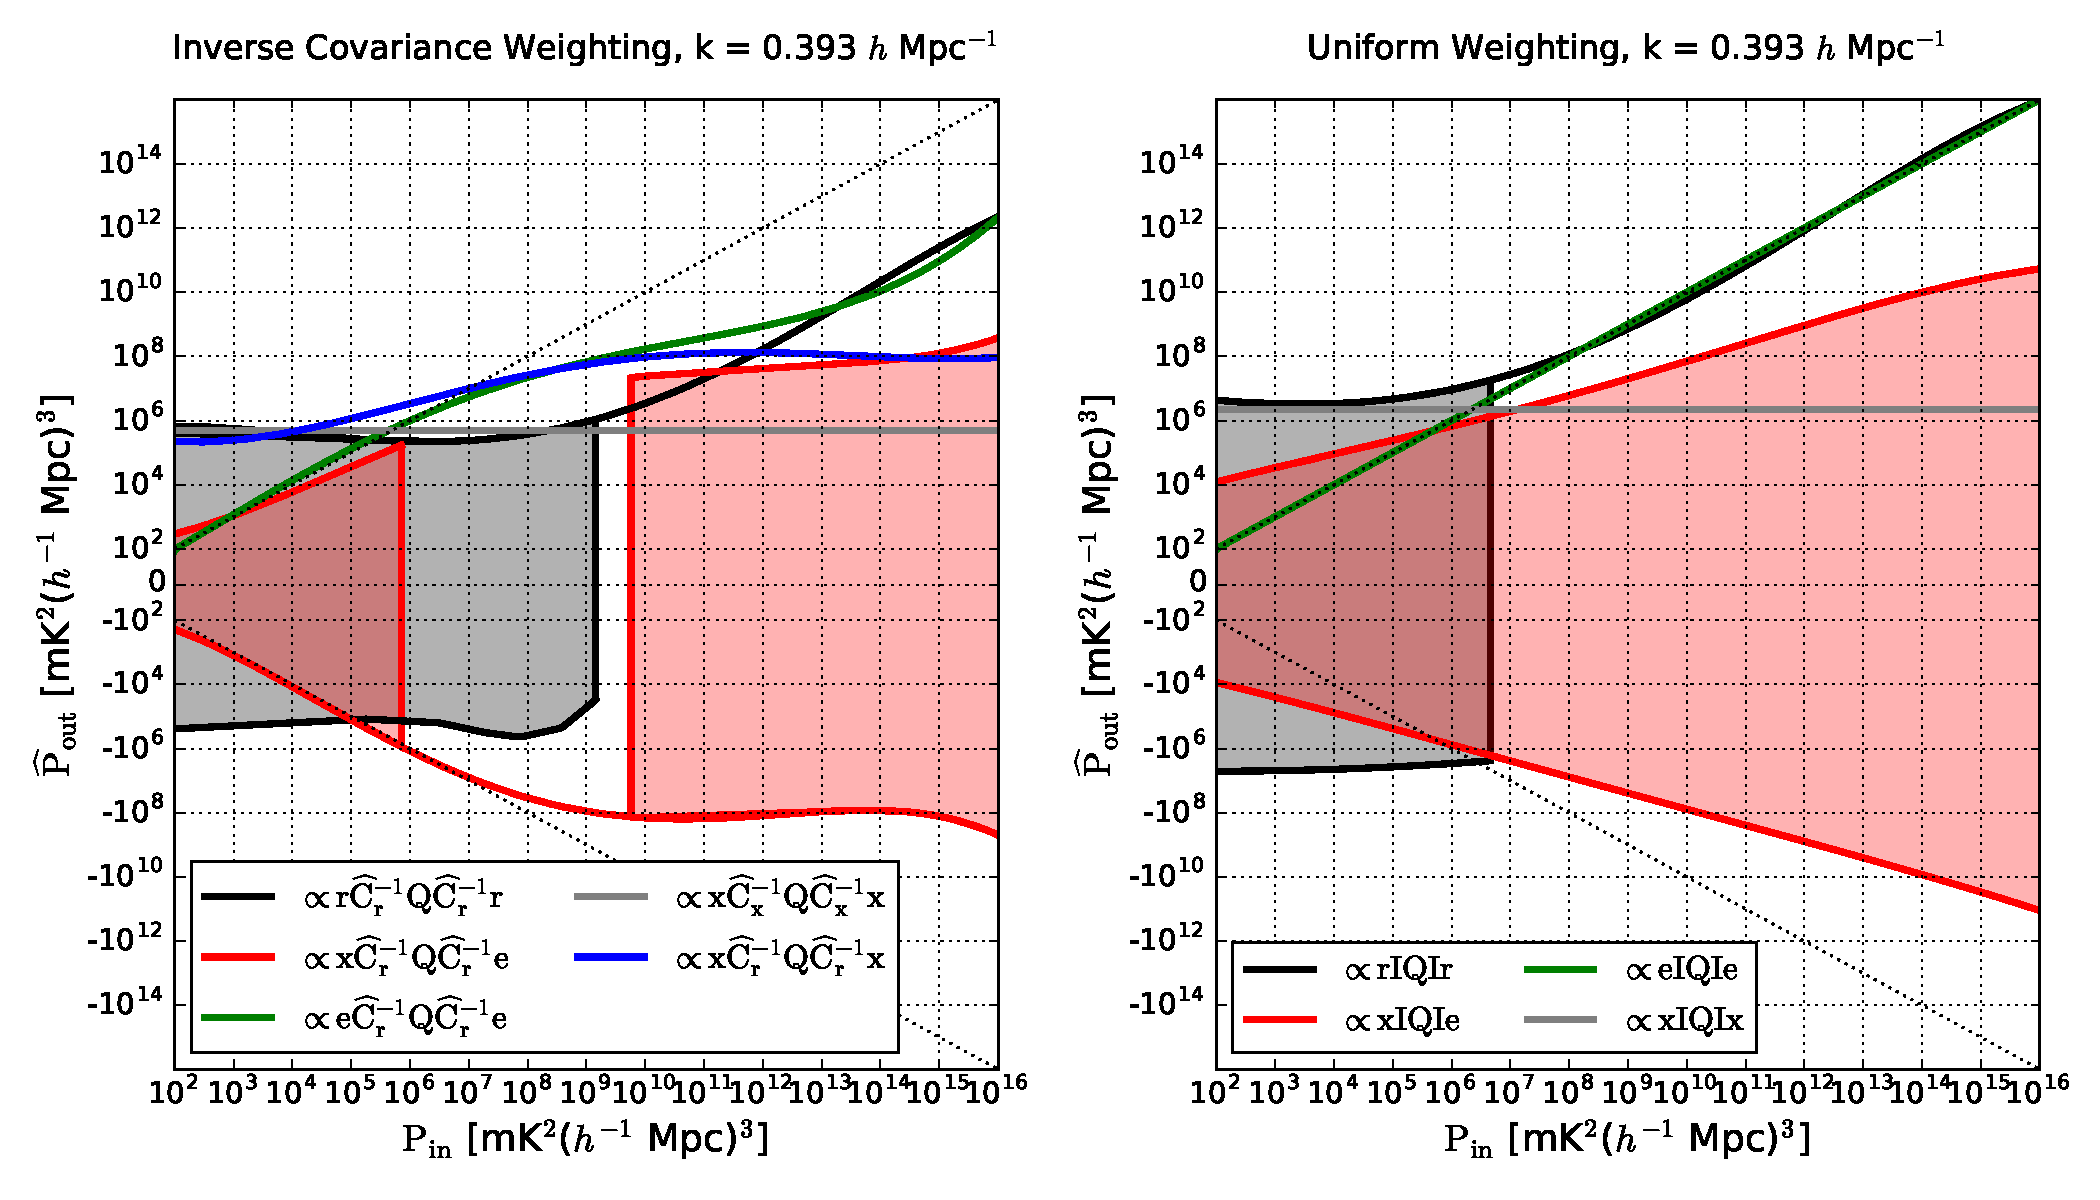
\includegraphics[width=1\textwidth]{plots/sigloss_terms.pdf}
	\caption{Illustration of the power spectrum amplitude of various power spectrum terms as a function of injected EoR power level summed into the 
data. Left: The empirically estimated inverse covariance weighted case used in \citetalias{ali_et_al2015}. The output power spectrum ($\widehat{P}_{\rm out}=\widehat{\textbf{P}}_r$) is shown in black, and the individual terms in Equation 
\eqref{eq:crossterm} are shown in blue, red, and green. The dotted diagonal black line indicates perfect 1:1 input-to-output mapping (no signal loss). The details of the simulation used to generate the figure is explained in Section 
\ref{sec:Practice}; here we sample a larger $P_{\rm in}$ range and fit smooth polynomials to our data points to make an illustrative example.  The gray 
horizontal line is the power spectrum value of data alone, $\widehat{\textbf{P}}_{x}$ (it does not depend on injected power). The green signal-signal 
component is the term used in \citetalias{ali_et_al2015} to estimate signal loss. It is significantly higher 
than $\widehat{\textbf{P}}_{r}$ (black) when the cross-terms (red) are large and negative (black $=$ green $+$ red $+$ blue) . In the 
regime where cross-correlations between injection and data are not dominant (small and large $P_{\rm in}$), the cross-terms have a noise-like 
term with width $\sqrt{\widehat{\textbf{P}}_e}\sqrt{\widehat{\textbf{P}}_x}$. However, at power levels comparable to the data (the middle region), the cross-terms can produce large, negative signal due to the couplings between $\textbf{x}$ and $\textbf{e}$ which affect 
$\widehat{\textbf{C}}_{r}$. This causes the difference between the green curve (which exhibits negligible loss at 
the data-only power spectrum value) and the black curve (which exhibits $\sim$$4$ orders of magnitude of loss). Right: The same power spectrum terms illustrated for the uniform weighted case.}
	\label{fig:sigloss_terms}
\end{figure*}

The source of the strong negative cross-term is not immediately obvious, however it is an explainable effect. 
When $\textbf{R}_{r}$
is taken to be $\widehat{\textbf{C}}_{r}^{-1}$, the third term of Equation \eqref{eq:crossterm} is a cross-correlation between $\widehat{\textbf{C}}_{r}^{-1}\textbf{x}$ and
$\widehat{\textbf{C}}_{r}^{-1}\textbf{e}$. As shown in \citet{switzer_et_al2015}, this cross-correlation term is non-zero, and in fact negative in expectation. 
This negative cross-term power arises from a coupling between the inverse of 
$\widehat{\textbf{C}}_{r}$ and $\mathbf{x}$. 
Intuitively, we can see this by expanding the empirical covariance of $\textbf{r}=\textbf{x}+\textbf{e}$:

\begin{eqnarray}
\widehat{\textbf{C}}_{r} &=& \langle \textbf{rr}^{\dagger} \rangle_{t} \nonumber \\ 
&=& \langle \textbf{xx}^{\dagger} \rangle_{t} + \langle \textbf{xe}^{\dagger} \rangle_{t} + \langle \textbf{ex}^{\dagger} \rangle_{t} + \langle 
\textbf{ee}^{\dagger} \rangle_{t},
\end{eqnarray}

\noindent where we can neglect the first term because $\textbf{x}$ is small (i.e. the large negative cross-term power in the left panel of Figure \ref{fig:sigloss_terms} occurs when the injected amplitude surpasses the level of the data-only power spectrum).  Without loss of generality, we will assume
an eigenbasis of $\textbf{e}$, so that $\langle 
\textbf{ee}^{\dagger} \rangle_{t}$ is diagonal. The middle 
two terms, however, can have power in their off-diagonal terms due to the fact that, when averaging over a finite
ensemble, $\langle\textbf{xe}^\dagger\rangle_t$ is not zero.  As shown in Appendix C of \citet{parsons_et_al2014}%\footnote{This same appendix also gives a now-prescient warning about signal loss and the dangers of noise and sample variance in inverse covariance.}
, to leading order the inversion of a diagonal-dominant matrix like $\widehat{\textbf{C}}_{r}$ (from $\langle 
\textbf{ee}^{\dagger} \rangle_{t}$) with smaller
off-diagonal terms results in a new diagonal-dominant matrix with negative off-diagonal terms. These off-diagonal
terms depend on both $\textbf{x}$ and $\textbf{e}$. Then, when $\widehat{\textbf{C}}^{-1}_{r}$ is multiplied into $\textbf{x}$,
the result is a vector that is similar to $\textbf{x}$ but
contains a residual correlation to $\textbf{e}$ from the off-diagonal components of $\widehat{\textbf{C}}^{-1}_{r}$. The
correlation is negative because the product $\widehat{\textbf{C}}_r^{-1}\textbf{x}$ effectively squares the $\textbf{x}$-dependence
of the off-diagonal terms in $\widehat{\textbf{C}}^{-1}_{r}$ while retaining the negative sign that arose from the inversion
of a diagonal-dominant matrix.
% XXX [ARP: we may want to write this all out explicitly in an appendix]

%The correlation between $\widehat{\textbf{C}}_r^{-1}\textbf{e}$ and $\widehat{\textbf{C}}_r^{-1}\textbf{x}$ means that we cannot compute signal loss using a signal-only 
%simulation, which would yield greater values for $\widehat{P}_{\rm out}$ and thereby underestimate signal loss. This argument is also made in \citet{switzer_et_al2015} in regards to estimating loss associated with the foreground cleaning of Green Bank Telescope (GBT) data. Therefore, in our revised 
%signal loss computation we use the full quantity for $\widehat{P}_{\rm out}$ as defined in Equation \eqref{eq:crossterm_full}.
%weighted power spectrum of the data from the weighted power spectrum of data plus EoR. 

%\dcj{This paragraph has me confused.}
%The conclusion is that signal loss generically arises because of couplings between $\widehat{\textbf{C}}^{-1}_{r}$ and $\mathbf{x}$. In principle, using $\widehat{\textbf{C}}^{-1}_{r}$ in place of the true inverse covariance $\textbf{C}^{-1}$ provides yet another source of multiplicative bias, which results in a modification to the treatment shown here. Such a modification is accounted for in the demonstration of Appendix \ref{sec:sigloss_appendix}, where we additionally discard the assumption that $|\textbf{x}|\ll|\textbf{e}|$. However, despite the loosening of these approximations, one sees that the qualitative message (of anti-correlations resulting in signal loss) remains intact.

{\bf In general:} Another way to phrase the shortcoming of the empirical inverse covariance estimator (which is also discussed in Appendix \ref{sec:sigloss_appendix}) is that it is not properly normalized. Signal loss due to couplings between the data and its weightings arise because our unnormalized quadratic estimator from Equation \eqref{eq:qhat} ceases to be a quadratic quantity, and instead contains higher order powers of the data. However, the normalization matrix $\mathbf{M}$ is derived assuming that the unnormalized estimator is quadratic in the data. The power spectrum estimate will therefore be incorrectly normalized, which manifests as signal loss. We leave a full analytic solution for $\mathbf{M}$ for future work, since our simulations already capture the full phenomenology of signal loss and have the added benefit of being more easily generalizable in the face of non-Gaussian systematics.

\subsubsection{Signal Loss in Practice}
\label{sec:Practice}

We now shift our attention towards computing upper limits on the EoR signal for the fringe-rate filtered PAPER-64 dataset in a way that accounts for signal loss. While our methodology 
outlined below is independent of weighting scheme, here we demonstrate the computation using empirically estimated inverse covariance weighting 
($\textbf{R} \equiv \widehat{\textbf{C}}^{-1}$), the weighting scheme used in \citetalias{ali_et_al2015} which leads to substantial loss. With this weighting, our 
expressions for $\widehat{P}_{\rm in}$ and $\widehat{P}_{\rm out}$ become:

\begin{eqnarray}
\widehat{P}_{\rm in,\alpha} &=&  \text{M}^{\alpha}_{\rm in}\textbf{e}^{\dagger}\textbf{I}\textbf{Q}^{\alpha}\textbf{I}\textbf{e} \\
\widehat{P}_{\rm out,\alpha} &=&  \text{M}^{\alpha}_{r}\textbf{r}^{\dagger}\widehat{\textbf{C}}_{r}^{-1}\textbf{Q}^{\alpha}\widehat{\textbf{C}}_{r}^{-1}\textbf{r}.% \nonumber \\
%&&\phantom{=====} 
%-  \text{M}^{\alpha}_{x}\textbf{x}^{\dagger}\widehat{\textbf{C}}_{x}^{-1}\textbf{Q}^{\alpha}\widehat{\textbf{C}}_{x}^{-1}\textbf{x}. 
\end{eqnarray}

%The treatment we outlined in the previous section implicitly assumed that signal loss corrections could be treated in expectation. In practice, however, the signal loss itself is a random variable --- some realizations of the cosmological signal may be more correlated with foreground modes than others, leading to more signal loss. This leads to two issues. The first is that Equation \eqref{eq:LinearPspecSum} may not hold. In particular, a third term that is a quadratic combination of $\f$ and $\s$ (e.g., $\f^\dagger \C^{-1} \s$) may appear. However, we can circumvent this issue by decomposing $\f$ into a sum of two vectors, one that is proportional to $\s$ and one that is orthogonal to $\s$. The former can be absorbed into the EoR term (part of the signal loss estimate), while the latter can be absorbed into the foreground term. In other words, suppose that we have
%\begin{equation}
%\phat_x \approx \ell_{\rm fg} |\mathbf{f}|^2 + \ell_{\rm eor} |\mathbf{e}|^2 + \ell_{\rm fe} \mathbf{f} \cdot \mathbf{e}.
%\end{equation}
%in place of Equation \eqref{eq:LinearPspecSum}. Now, split $\mathbf{f}$ into $\mathbf{ f}_\parallel +\mathbf{ f}_\perp$, which are the components of the foregrounds that couple to the EoR versus those that do not. Further parameterize $\mathbf{ f}_\parallel \equiv \rho \mathbf{e}$, where $\rho$ is some correlation coefficient that quantifies the degree of correlation between the foregrounds and the EoR. This then gives
%\begin{equation}
%\label{eq:fperpfpara}
%\phat_x \approx \ell_{\rm fg} |\mathbf{f}|^2 +( \ell_{\rm eor} + \rho  \ell_{\rm fe} ) |\mathbf{e}|^2 + \ell_{\rm fe} \mathbf{f}\cdot \mathbf{f}_\perp.
%\end{equation}
%Since $|\mathbf{e}|^2$ would be a lossless estimate of the true EoR power spectrum, this expression recovers the linear relation between the true EoR power spectrum and the lossy estimate.
%\dcj{Wait what? I think you are saying essentially that some x can remain in Pout which is what we are seeing. Or is this some extra bit of method which has been added to the analysis...} \acl{I'm not sure that's what I'm saying. (And by ``I'm not sure" I don't mean it in the colloquial sense of ``you're not right and I'm just trying to be polite about it", but rather the literal sense of the phrase ``I'm not sure"). What I was trying to say was that if I wrote Equation \eqref{eq:LinearPspecSum} without the ensemble average, I could say
%\begin{equation}
%\phat_x \approx \ell_{\rm fg} f^2 + \ell_{\rm eor} e^2 + \ell_{\rm fe} fe.
%\end{equation}
%(Note that even this is an approximation. In principle there is an infinite series containing all possible powers of 
%$e$ and $f$). Now, we split $f$ into $ f_\parallel + f_\perp$, which are the components of the foregrounds that 
%couple to the EoR versus those that do not. Further parameterize $f_\parallel \equiv \rho e$, where $\rho$ is 
%some correlation coefficient that quantifies the degree of correlation between the foregrounds and the EoR. 
%Under this parameterization, one can write the $fe$ term in terms of $e^2$ (which gets absorbed into the other 
%EoR term, plus residual foregrounds that we don't care about).}\acl{Just promoted this last part to something in 
%the main text.}\dcj{I will admit to being a little lost here.  Doesn't changing the basis just convert the unknown f 
%dot s term into other unknown terms. Isn't the whole point of Eq 24 supposed to be that we can subtract off the 
%$g(x)$ to estimate $\hat{\ell}_{\rm eor}$?  How do we subtract off $f\dot f_\perp$? Don't we want to know $
%\ell_{\rm eor}$ not $(\ell_{\rm eor} + \rho\ell_{\rm fe})$? }
%\acl{I think what we are trying to say here is that actually the thing we want \emph{is} $(\ell_{\rm eor} + \rho\ell_{\rm fe})$. Essentially, the potential coupling between the injected EoR and the foregrounds means that we lose the nice form of Equation \eqref{eq:LinearPspecSum}, which justified what is basically a multiplicative correction to signal loss. What we are suggesting here is that even when there is a coupling, the estimator can be parameterized as $\alpha  |\mathbf{e}|^2 + \beta$. So essentially we are defining an effective $
%\ell_{\rm eor}$, which is given by $(\ell_{\rm eor} + \rho\ell_{\rm fe})$.}

One issue to address is how one incorporates the randomness of $\widehat{P}_{\rm out}$ into our signal loss corrections. A different realization of the mock EoR signal is injected with each bootstrap run, causing the output to vary in three ways ---  there is noise variation from the bootstraps, there is cosmic variation from generating multiple realizations of the mock EoR signal, and there is a variation caused by whether the injected signal looks more or less ``like'' the data (i.e. how much coupling there is, which affects how much loss results). 

For each injection level, the true $P_{\rm in}$ is simply the average of our bootstrapped estimates $\widehat{P}_{\rm in}$, since $\widehat{P}_{\rm in, \alpha}$ is by construction an unbiased estimator. Phrased in the context of Bayes' rule, we wish to find the posterior probability distribution $p(P_{\rm in} | 
\widehat{P}_{\rm out})$, which is the probability of $P_{\rm in}$ given the uncorrected/measured power spectrum estimate $\widehat{P}_{\rm out}$.  Bayes' rule relates the posterior, which we don't know, to the likelihood, which we can forward model. In other words,

\begin{equation}
\label{eq:Bayes}
p(P_{\rm in} | \widehat{P}_{\rm out}) \propto {\mathcal{L} (  \widehat{P}_{\rm out} | P_{\rm in})}\,p(P_{\rm in}) ,
\end{equation}

\noindent where $\mathcal{L} $ is the likelihood function defined 
as the distribution of data plus injection ($\widehat{P}_{\rm out}$) given the injection $P_{\rm in}$.  We construct this distribution  
by fixing $P_{\rm in}$ and simulating our analysis pipeline for many realizations of the injected EoR signal 
consistent with this power spectrum. The resulting distribution is normalized such that the sum over $\widehat{P}_{\rm out}$ is unity, and the 
whole process is then repeated for a different value of $P_{\rm in}$. 

%\subsubsection{Signal Loss Implementation Details}
%\label{sec:Implementation}

The implementation details of the injection process require some more detailed explanation. In our code, we add a new realization of EoR to each independent bootstrap of data (see Section \ref{sec:Boot} for a description of PAPER's bootstrapping routine) with the goal of simultaneously capturing cosmic variance, noise variance, and signal loss. To limit computing time we perform $20$ realizations of each $P_{\rm in}$ level. We also run $50$ total EoR injection levels, yielding $P_{\rm in}$ values that range from $\sim$$10^{5}$\,mK$^{2}$ ($h^{-1}$ Mpc)$^{3}$ to $\sim$10$^{11}$\,mK$^{2}$ ($h^{-1}$ Mpc)$^{3}$, resulting in a total of $1000$ data points on our $P_{\rm in}$ vs. $\widehat{P}_{\rm out}$ grid. 

Going forward, we treat every $k$-value separately in order to determine an upper limit on the EoR signal per $k$. We bin our simulation outputs along the $P_{\rm in}$ axis (one bin per injection level) and, since they are well-approximated by a Gaussian distribution in our numerical results, we smooth the distribution of $\widehat{P}_{\rm out}$ values by fitting Gaussians for each bin based on its mean and variance (and normalize them). Stitching all of them together results in a 2-dimensional transfer function --- the likelihood function in Bayes' rule, namely $\mathcal{L} (  \widehat{P}_{\rm out} | P_{\rm in})$. We then have a choice for our prior, $p(P_{\rm in})$, and we choose to invoke a Jeffreys prior (\citealt{jaynes1968}) because it is a true uninformative prior. For a derivation and more details about the Jeffreys prior used in our analysis, see Appendix \ref{sec:jeffreys}.

Finally, our transfer functions are shown in Figure \ref{fig:sigloss_transfercurve} for both the weighted (left) and unweighted (right) cases. Our bootstrapped power spectrum outputs are shown as black points and the colored heat-map overlaid on top is the likelihood function modified by our prior. Although we only show figures for one $k$-value, we note that 
the shape of the transfer curve is similar for all $k$'s. We then invoke Bayes' interpretation and re-interpret it as the posterior $p(P_{\rm in}|\widehat{P}_{\rm out})$ where we recall that $\widehat{P}_{\rm out}$ is a model of our data. To do this we make a horizontal cut across at the data value $\widehat{\textbf{P}}_{x}$ (setting $\widehat{P}_{\rm out} = \widehat{\textbf{P}}_{x}$), shown by the gray solid line, to yield a posterior distribution for the signal. We normalize this final distribution and compute the $95\%$ confidence interval (an upper limit on EoR).

%We note that the distribution of $\phat_{x}$ has a variance determined from the bootstrapping process and is peaked around the power spectrum value computed from the no-bootstrapping case. We smooth its distribution using 1D kernel density estimators (and normalize to unity) before multiplying it with the transfer function. Performing a summation and normalization for the entire distribution of $\phat_{x}$ yields a final $P_{\rm in}$ distribution --- the distribution of our data as seen through the signal loss lens. We compute power spectrum points from the peak of the histograms, and power spectrum errors from $95\%$ confidence intervals. 

By-eye inspection of the transfer function in Figure \ref{fig:sigloss_transfercurve} gives a sense of what the signal loss result should be. The power spectrum value of our data, $
\widehat{\textbf{P}}_{x}$ is marked by the solid gray horizontal lines. From the left plot (empirically estimated inverse covariance weighting), one can eyeball that a data value of $10^{5} \,$mK$^{2}$ ($h^{-1}$ Mpc)$^{3}$, for example, would map approximately to an upper limit of $\sim10^{9} \,$mK$^{2}$ ($h^{-1}$ Mpc)$^{3}$, implying a signal loss factor of $\sim10^{4}$. For the uniform-weighted case (right plot), we see no loss at a data value of $\sim10^{7} \,$mK$^{2}$ ($h^{-1}$ Mpc)$^{3}$.

%As a final complication to our procedure, we note that there will be some scatter in our likelihood due to our having only a finite number of simulations. Ideally, running many simulations would lead to convergence; however, our desire to be able to quickly and easily estimate signal loss for a variety of weighting schemes and datasets means having a finite sample in practice. \dcj{This dependence on injection count was checked with a run having 10x the usual number of integrations.} To separate the intrinsic stochasticity of signal loss from that which arises due to simulation sample variance, we repeat our analysis for a power spectrum estimator without signal loss ($\textbf{R} = \textbf{I}$), shown as the right plot in Figure \ref{fig:sigloss_transfercurve}. Here the scatter, evident as deviations from unity-transfer, is entirely due to finite sample variance. To remove this effect we measure the width of this lossless case and then de-convolve that extra width from the likelihood for the lossy scenario. Specifically, we de-convolve Gaussian distributions of $\widehat{P}_{\rm out}$ in the uniform-weighted case from those of the weighted case (vertical cuts through the plots in Figure \ref{fig:sigloss_transfercurve}), for every $P_{\rm in}$. By doing this, we are left with only the intrinsic scatter in signal loss, or scatter that stems from how much the random EoR signal $\textbf{e}$ happens to 
%look like the data $\textbf{x}$, a quantity we do not know offhand but one that we would like to correct for. As an extreme example, if we are very unlucky, one realization of $\textbf{e}$ would have the same shapes, or eigenvectors, as $\textbf{x}$. An empirically-derived covariance would then down-weight these shapes, destroying the entire EoR signal. On the other hand, the less that $\textbf{e}$ looks like $\textbf{x}$, the less signal loss that would result. The intrinsic scatter we can get is not a dominant factor in this case but it is important to correct for the fact that a particular $\widehat{P}_{\rm out}$ value could arise from a range of $P_{\rm in}$ values. 

%The solid black diagonal line in Figure \ref{fig:sigloss_transfercurve} shows unity-transfer, which we expect to occur for the 
%nweighted case ($\textbf{R} = \textbf{I}$). Therefore, it is worth thinking about the spread, or scatter, around this black line that 
%we see in the right plot (the colored `heat-map'). One might imagine that there should be one true $\widehat{P}_{\rm out}$ value for every 
%$P_{\rm in}$, implying one well-determined signal loss factor for every data value. Focusing on the unweighted case alone, the 
%scatter observed arises from the fact that the values of the cross-terms involving $\textbf{e}$ and $\textbf{x}$ in Equation 
%\eqref{eq:pout_expand} change for different mock EoR signals, $\textbf{e}$. Since we draw different random $\textbf{e}$'s for 
%every bootstrap (for reasons made clear in the next paragraph), there is a range of $\widehat{P}_{\rm out}$ values that results from the same 
%$P_{\rm in}$. This randomness causes the spread seen in the right plot of Figure \ref{fig:sigloss_transfercurve}, as well as most of 
%the spread in the weighted case (left plot).

\begin{figure*}
	\centering
	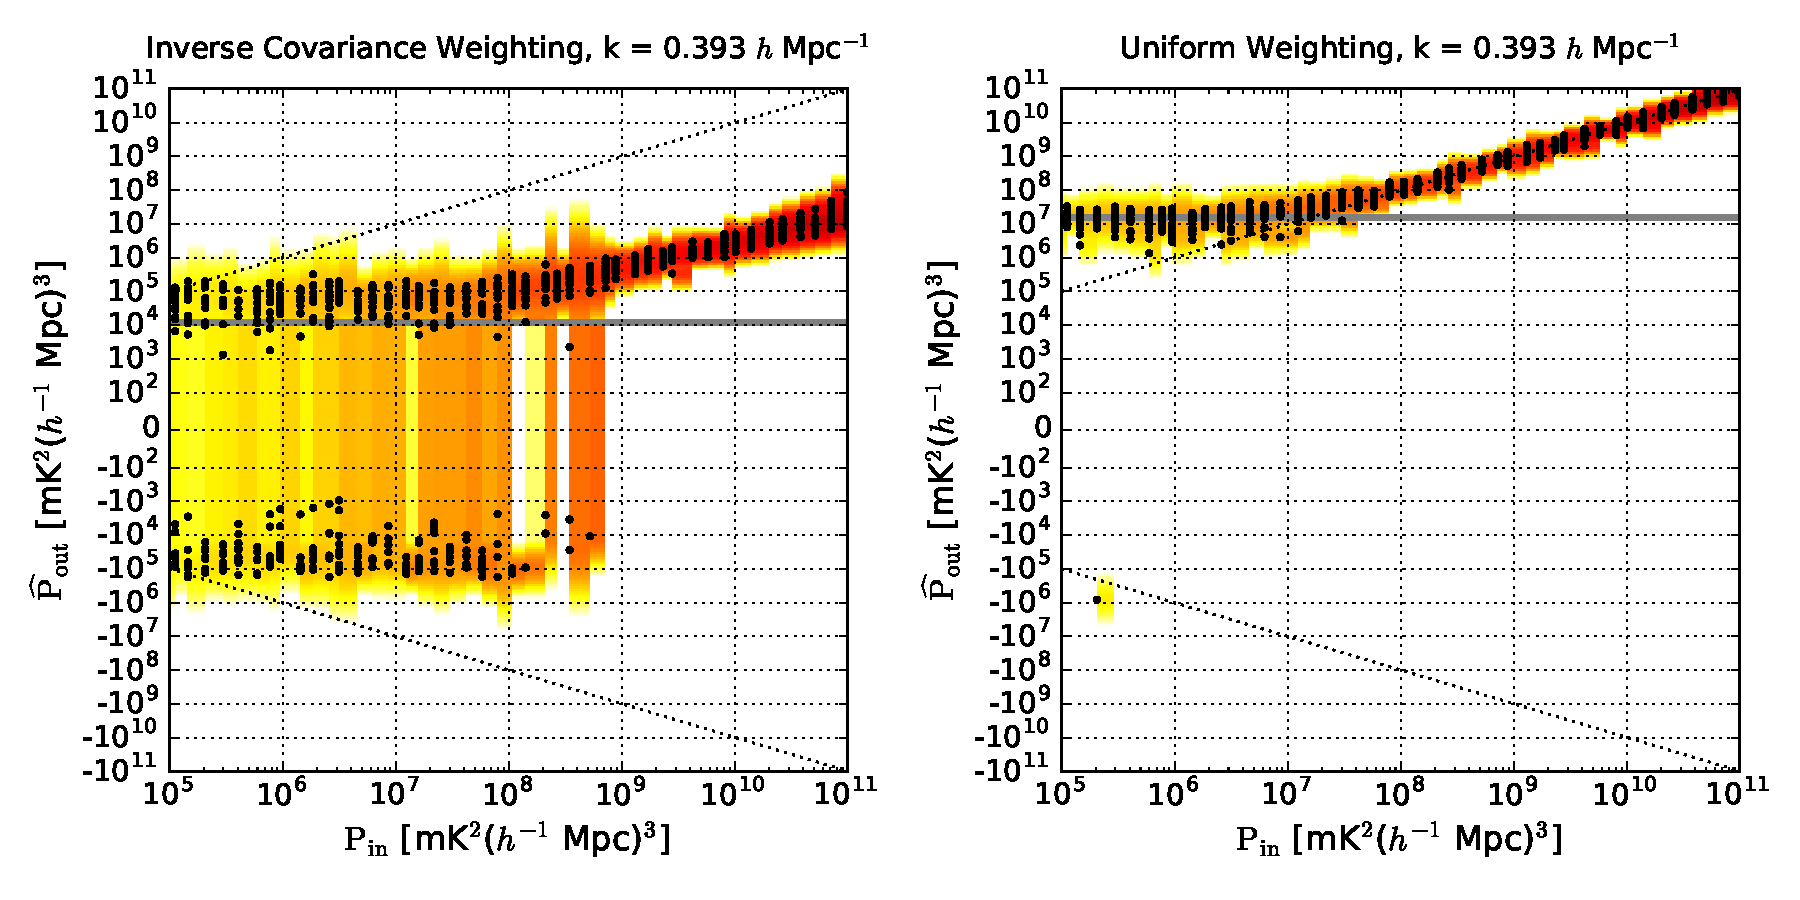
\includegraphics[width=1\textwidth]{plots/sigloss_transfercurve_posneg.pdf}
	\caption{Signal loss transfer functions showing the relationship of $P_{\rm in}$ and $\widehat{P}_{\rm out}$, as defined by Equations \eqref{eq:Pin} and \eqref{eq:sigloss}. Power spectra values (black points) are generated for $20$ realizations of $\textbf{e}$ per signal injection level. Since our $\widehat{P}_{\rm out}$ values are well-approximated by a Gaussian distribution, we fit Gaussians to each injection level based on the mean and variance of the simulation outputs. This entire likelihood function is then multiplied by a Jeffreys prior for $p(P_{\rm in}$), with the final result shown as the colored 
heat-maps on top of the points. Two cases are displayed: empirically estimated inverse covariance weighted PAPER-64 data (left) and uniform-weighted data (right). The dotted black 
diagonal lines mark a perfect unity mapping, and the solid gray horizontal line denotes the power spectrum value of the data $\widehat{\textbf{P}}_{x}$, from which a posterior distribution for the signal is extracted. From these plots, it is clear that the weighted case results in $\sim4$ orders of magnitude of signal loss at the data-only power spectrum value, whereas the uniform-weighted case does 
not exhibit loss. The general shape of these transfer functions are also shown by the black curves in Figure \ref{fig:sigloss_terms} for comparison.}
	\label{fig:sigloss_transfercurve}
\end{figure*}

%One peculiar aspect of Figure \ref{fig:sigloss_transfercurve} is the fact that at low $P_{\rm in}$ values it appears that we can have signal gain ($\widehat{P}_{\rm out} > P_{in}$). \cc{This is a log-plotting effect and is under-construction!}.
%This is unphysical in nature but caused due to the dominating cross-terms involving $\textbf{e}$ and $\textbf{x}$ in Equation \eqref{eq:pout_expand} once $\textbf{e}$ becomes small. 
%
%The shape of our signal loss transfer function can be described as follows. At low injection levels, for small $\textbf{e}$, we are dominated by the cross-terms involving $\textbf{e}$ and $\textbf{x}$ in Equation \eqref{eq:pout_expand}. As $\textbf{e}$ increases, we move 
%into a regime where $\widehat{P}_{\rm out} \sim P_{in}$, and then eventually into a regime where $\widehat{P}_{\rm out} < P_{in}$ when $\textbf{e}$ is 
%large enough to be destroyed if weighting the data using itself. Although we only show figures for one $k$ value, we note that 
%the shape of the transfer curve is nearly identical for all $k$'s (though we treat each $k$ separately).

%\begin{figure*}
%	\centering
%	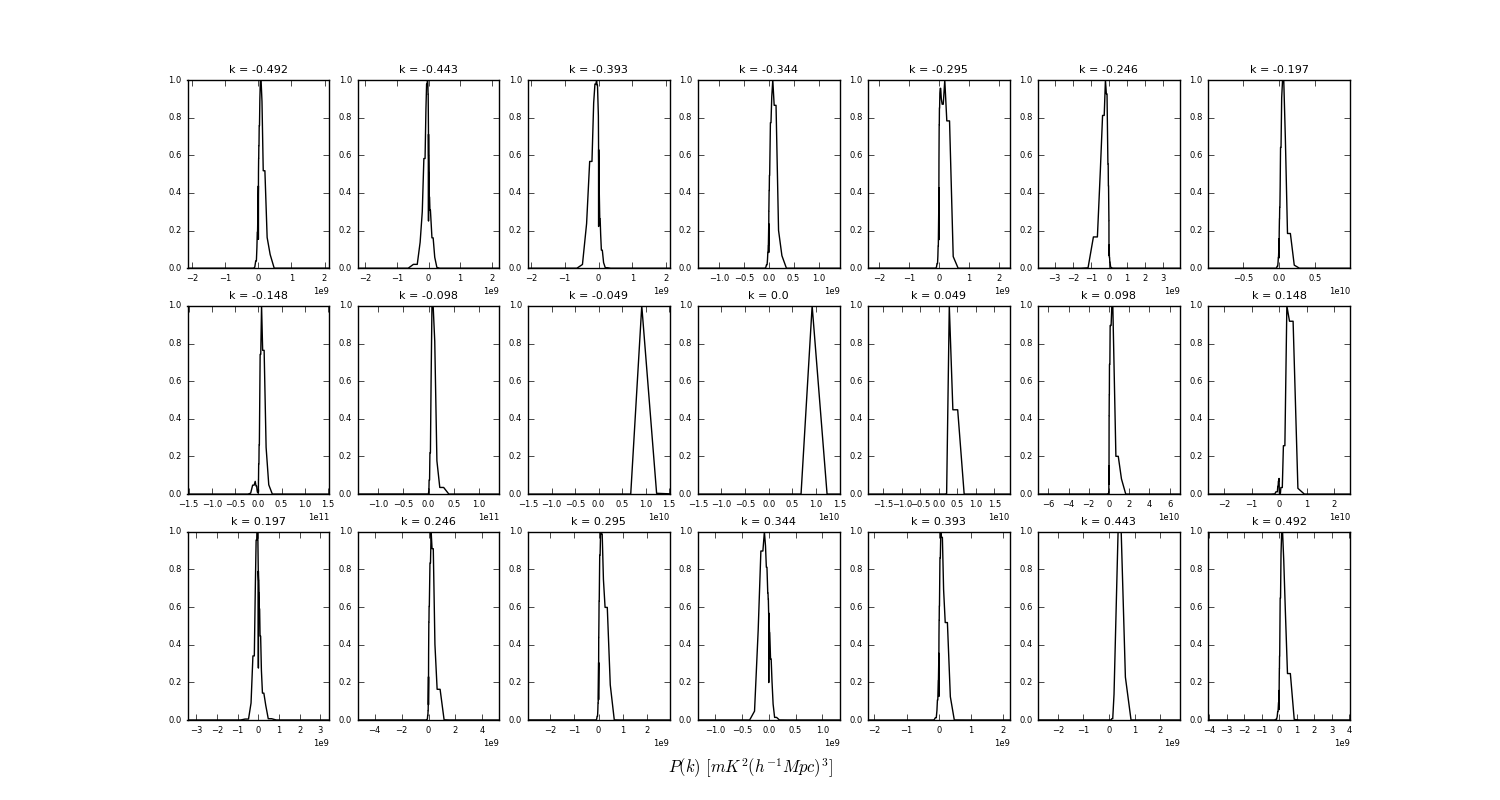
\includegraphics[trim={1cm 0cm 1cm 1cm},width=1\textwidth]{plots/sigloss_datadist_inversecovariance.png}
%	\caption{Normalized histograms of the power spectra that result from using inverse covariance weighting on %PAPER-64 data after signal loss correction. Power spectrum points are computed from the peak of the distributions. Errors are computed using $95\%$ confidence intervals.}
%	\label{fig:sigloss_datadist_inversecovariance}
%\end{figure*}

The loss-corrected power spectrum limit for empirically estimated inverse covariance weighted PAPER-64 data is shown in Figure \ref{fig:ps2_data} (solid red), which we can compare to the original lossy result (dashed red). %There are a few important checks to examine. First, we see that the uniform-weighted power spectrum $2\sigma$ upper limit (dashed blue) is identical in both panels. This is an important check, as we expect no signal loss for this case. Any difference here would indicate an error in the pipeline or discrepancy in the range of data included. Additionally, it is clear that the power spectrum, prior to signal loss estimation, is inconsistent with the (now revised) theoretical noise level prediction. 
Post-signal loss estimation, the power spectrum limits are higher than both the theoretical noise level (green) and uniform-weighted power spectrum (which is shown three ways: black and gray points are positive and negative power spectrum values, respectively, with $2\sigma$ error bars, the solid blue is the upper limit on the EoR signal using the full signal injection framework, and the shaded gray is the power spectrum values with thermal noise errors). We elaborate on this point in the next section, as well as investigate alternate 
weighting schemes to inverse covariance weighting, with the goal of finding one that balances the aggressiveness of down-weighting contaminants and minimizing the loss of the EoR signal. 

\begin{figure*}
	\centering
	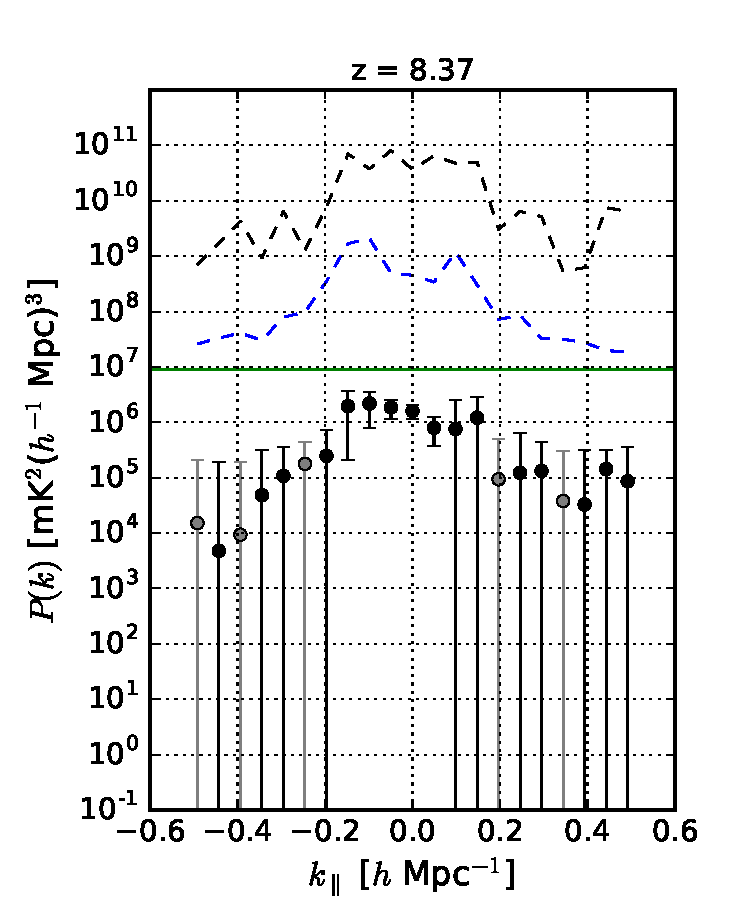
\includegraphics[width=0.4\textwidth]{plots/ps1_data.pdf}
	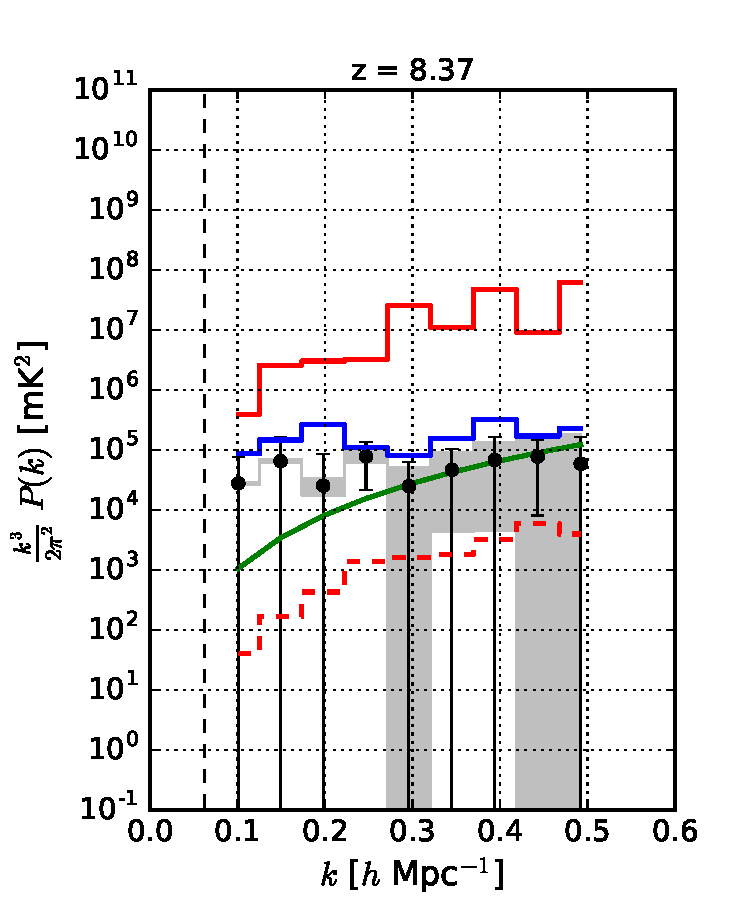
\includegraphics[width=0.4\textwidth]{plots/ps2_data.pdf}
	\caption{A power spectrum of a subset of PAPER-64 data illustrating the use of empirical inverse covariance weighting. The solid red curve is the $2\sigma$ upper limit on the EoR signal estimated from our signal injection framework using empirical inverse covariance weighting. Shown for comparison is the lossy limit prior to signal loss estimation (dashed red). The theoretical $2\sigma$ thermal noise level prediction based on observational parameters is in green, whose calculation is detailed in Section \ref{sec:PSSense}. Additionally, the power spectrum results for the uniform weighted case is shown in three different ways: power spectrum values (black and gray points as positive and negative values, respectively, with $2\sigma$ error bars), the $2\sigma$ upper limit on the EoR signal using our full signal injection framework (solid blue), and the measured power spectrum values with $2\sigma$ thermal noise errors (gray shaded regions). The vertical dashed black lines signify the horizon limit for this analysis using $30$\,m baselines.}
\label{fig:ps2_data}
\end{figure*}


\subsubsection{Minimizing Signal Loss}
\label{sec:Weight}

With a signal loss formalism established, we now have the capability of experimenting 
with different weighting options for $\textbf{R}$. Our goal here is to choose a weighting method that successfully down-weights 
foregrounds and systematics in our data without generating large amounts of signal loss as we have seen with the inverse covariance estimator. We have found that the balance 
between the two is a delicate one and requires a careful understanding and altering of empirical covariances. 

We saw in Section \ref{sec:otherweight} how limiting the number of down-weighted eigenmodes (i.e. flattening out part of the 
eigenspectrum and effectively de-coupling the lowest-valued eigenmodes from the data, which converge to the true eigenspectrum the slowest and are often EoR-dominated) can help minimize signal loss. We experiment with this idea on PAPER-64 data, dialing the number of modes 
that are down-weighted from zero (which is equivalent to identity-weighting, or the uniform-weighted case) to $21$ (which is the full inverse 
covariance estimator). The power spectrum results for one $k$-value, both before and after signal loss 
estimation, are shown in the top panel in Figure \ref{fig:sigloss_modeloop}. We see that the amount of signal loss increases as weighting 
becomes more aggressive (dashed red). In other words, more EoR-dominated fluctuations are being overfit and 
subtracted as more modes are down-weighted. We also find that the power spectrum upper limit, post-signal loss estimation, 
increases with the number of down-weighted modes (solid red). The more modes we use in down-weighting, the stronger the coupling between the weighting and the data, and the greater the error we have in estimating the power spectrum. \citet{switzer_et_al2013} took a similar approach in determining the optimal number of modes to down-weight in GBT data, finding similar trends and noting that removing too few modes is limited by residual foregrounds and removing too many modes is limited by large error bars and signal loss.

Optimistically, we expect there to be a `sweet spot' as we dial our regularization knob; a level of regularization where weighting 
is beneficial compared to uniform weighting (blue). In other words, we would like a weighting scheme that down-weights eigenmodes that predominantly describe foreground modes, but not EoR modes. We see in Figure \ref{fig:sigloss_modeloop} that this occurs roughly when 
only the $\sim2$-$3$ highest-valued eigenmodes are down-weighted and the rest are given equal weights (though for the case shown, weighting does not actually outperform uniform weighting). For a similar discussion on projecting out modes (zero-ing out eigenmodes, rather than just ignoring their relative weightings as we do in this study), see \citet{switzer_et_al2013}. 

We also saw in Section \ref{sec:otherweight} how adding the identity matrix to the empirical covariance can minimize signal loss. We experiment with this idea as well, shown in the bottom panel of Figure \ref{fig:sigloss_modeloop}. The dashed red and solid red lines represent power spectrum limits pre and post-signal loss estimation, respectively, as a function of the strength of $\textbf{I}$ that is added to $\widehat{\textbf{C}}$, quantified as the percentage of Tr($\widehat{\textbf{C}})\textbf{I}$ added to $\widehat{\textbf{C}}$. We parameterize this ``regularization strength" parameter as $\gamma$, namely $\widehat{\textbf{C}} \equiv \widehat{\textbf{C}} + \gamma$Tr$(\widehat{\textbf{C}})\textbf{I}$. From this plot we see that only a small percentage of Tr($\widehat{\textbf{C}})$ is needed to significantly reduce loss. We expect that as the strength of $\textbf{I}$ is increased (going to the left), both the red curves will approach the uniform-weighted case. We also notice that the post-signal loss limit hovers around the uniform-weighted limit for a large range of regularization strengths and while an overall trend from high-to-low signal loss is seen as the strength increases, there does not appear to be a clear `minimum' that produces the least loss.

\begin{figure*}
	\centering
	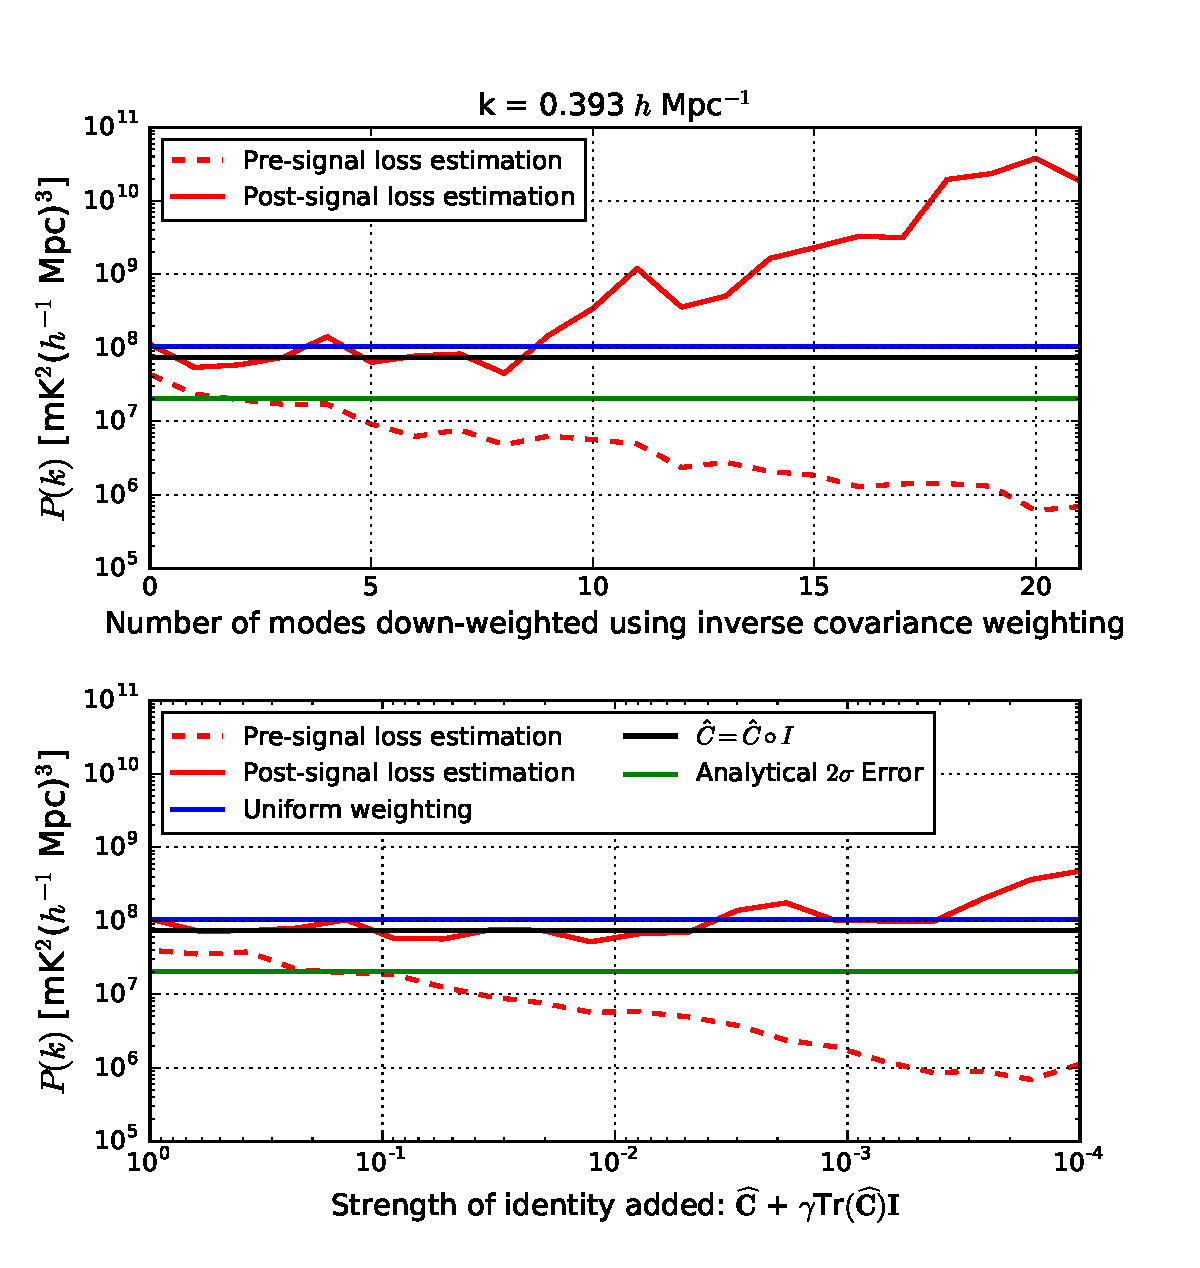
\includegraphics[width=1\textwidth]{plots/sigloss_modeloop_2panel.pdf}
	\caption{Power spectra $2\sigma$ upper limits for $k=0.393$\,$h$ Mpc$^{-1}$ for fringe-rate filtered PAPER-64 data. Top: Values 
are shown before (dashed red) and after (solid red) signal loss estimation via our signal injection framework as a function of number of eigenmodes of $\widehat{\textbf{C}}$ that 
are down-weighted. This regularization knob is tuned from $0$ modes on the left (i.e. unweighted) to $21$ modes on the right (i.e. the full inverse 
covariance estimator). Over $\sim3$ orders of magnitude of signal loss results when using empirically estimated inverse covariance weighting. Bottom: Power spectrum upper limits before (dashed red) and after (solid red) signal loss estimation as a function of identity added to the empirical covariance. This regularization knob is tuned from $\gamma = 10^{-4}$ on the right (i.e. very little regularization) to $\gamma = 1$ on the left (see main text for the definition of $\gamma$). Also 
plotted in both panels for comparison are $2\sigma$ power spectrum upper limits for the uniform-weighted case (blue) and inverse variance 
weighted case (black); both are after signal loss estimation. Finally, a theoretical prediction for noise ($2\sigma$ error) is plotted 
as green. In the PAPER-64 analysis in this paper, we choose to use a regularization scheme of $\widehat{\textbf{C}}_{\rm eff} \equiv 0.9 \, $Tr($\widehat{\textbf{C}})\textbf{I} + \widehat{\textbf{C}}$ ($\gamma = 0.9$) as a simple example of regularization that minimizes loss, and note that the power spectrum limits using this type of regularization are roughly constant across a large range of values of $\gamma$.}
	\label{fig:sigloss_modeloop}
\end{figure*}

In addition to our thermal noise prediction (green) and uniform-weighted power spectrum limit (blue), one additional horizontal line is shown in Figure \ref{fig:sigloss_modeloop} 
in both panels and represents a third regularization technique. This line (black) denotes the power spectrum value, post-signal loss estimation, for inverse variance weighting (multiplying an identity 
matrix element-wise to $\widehat{\textbf{C}}$). This result is single-valued and not a function of the horizontal axis. We see that all three regularization schemes shown (solid red, dashed red, black) perform similarly at 
their best (i.e. when $\sim2$-$3$ eigenmodes are down-weighted in the case of the solid red curve). However, for the remainder of this paper, we choose to use the weighting option of $\widehat{\textbf{C}} \equiv \widehat{\textbf{C}} + 0.9 \,$Tr($\widehat{\textbf{C}})\textbf{I}$, or $\gamma = 0.9$, which we will denote as $\widehat{\textbf{C}}_{\rm eff}$. We choose this weighting scheme merely as a simple example of regularizing PAPER-64 covariances, noting that the power spectrum upper limit remains roughly constant for a broad range of values of $\gamma$. We also note that all of the regularizations described here perform similarly to the uniformly weighted case. However, we find that the regularization of empirical covariances does outperform the uniform weighted case for redshifts (and $k$-values) for which there are stronger foregrounds, as presented in Kolopanis et al. (\textit{submitted}).

The power spectrum result for our subset of PAPER-64 data (using only one baseline separation type and $\widehat{\textbf{C}}_{\rm eff}$) is shown in Figure 
\ref{fig:ps1_data}. Again, the solid red curve represents our upper limit on the EoR signal using the full signal injection framework. The uniform weighted case is shown as the black and gray points, which correspond to positive and negative power spectrum values respectively (with 
$2\sigma$ errors bars). It is also shown as an upper limit using the signal injection framework (solid blue), which is interestingly larger than the errors computed from bootstrapping, likely because the full injection framework takes into account additional sample variance whereas the bootstrapped errors do not. Finally, the gray shaded regions combine the measured uniform weighted power spectrum values and the thermal noise. We show this power spectrum result as one example of how a simple regularization can minimize signal loss, though we also note that this weighting does not produce more stringent limits than the uniform weighted case. In Kolopanis et al. (\textit{submitted}), multiple redshifts are explored and found to benefit from weighting differently.

\begin{figure*}
	\centering
	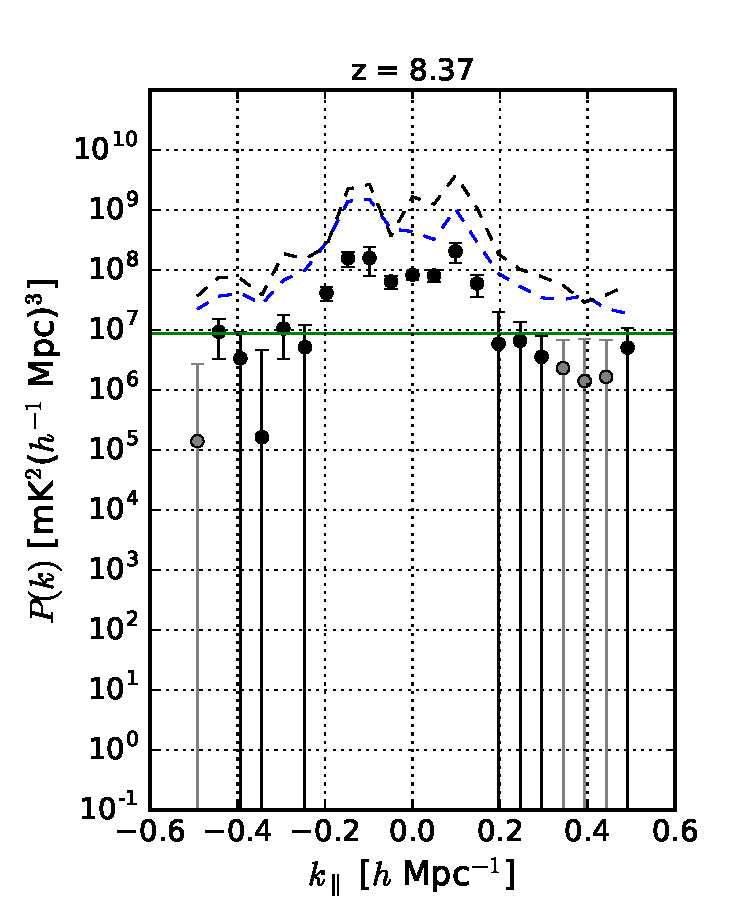
\includegraphics[width=0.4\textwidth]{plots/ps1_data_add.pdf}
	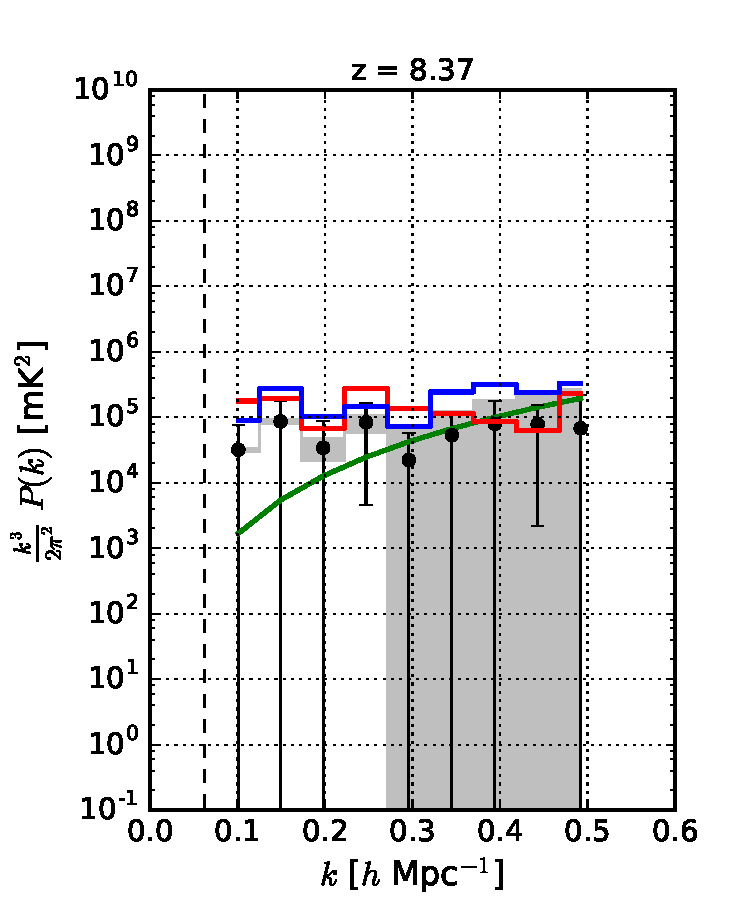
\includegraphics[width=0.4\textwidth]{plots/ps2_data_add.pdf}
	\caption{A power spectrum of a subset of PAPER-64 data illustrating the use of $\widehat{\textbf{C}}_{\rm eff}$ to minimize signal loss. The solid red curve is the $2\sigma$ upper limit on the EoR signal estimated from our signal injection framework. The theoretical $2\sigma$ thermal noise level prediction based on observational parameters is in green. Additionally, the power spectrum results for the uniform weighted case is shown in three different ways: power spectrum values (black and gray points as positive and negative values, respectively, with $2\sigma$ error bars), the $2\sigma$ upper limit on the EoR signal using our full signal injection framework (solid blue), and the measured power spectrum values with $2\sigma$ thermal noise errors (gray shaded regions). The vertical dashed black lines signify the horizon limit for this analysis using $30$\,m baselines. This power spectrum result does not use the full dataset's sensitivity as in \citetalias{ali_et_al2015} and Kolopanis et al. (\textit{submitted}), though we include all analysis changes which have mostly stemmed from revisions regarding signal 
loss, bootstrapping, and the theoretical error computation.}
	\label{fig:ps1_data}
\end{figure*}

In this section we have shown three simple ways of regularizing $\widehat{\textbf{C}}$ to minimize signal loss using PAPER-64 
data. There are many other weighting schemes that we leave for consideration in future work. For example, one could estimate 
$\widehat{\textbf{C}}$ using information from different subsets of baselines. For redundant arrays this could mean calculating $
\widehat{\textbf{C}}$ from a different but similar baseline type, such as the $\sim30$\,m diagonal PAPER baselines (instead of the 
horizontal E/W ones). Alternately, covariances could be estimated from all other baselines except the two being cross-multiplied 
when forming a power spectrum estimate. This method was used in \citet{parsons_et_al2014} (a similar method was also used in \citet{dillon_et_al2015}) in order to avoid suppressing the 
21\,cm signal, and it is worth noting that the PAPER-32 results are likely less impacted from the issue of signal loss underestimation 
because of this very reason (however, they are affected by the error estimation issues described in Section \ref{sec:Error}, so 
we also regard those results as suspect and superseded by those of Kolopanis et al. (\textit{submitted})).

Another possible way to regularize $\widehat{\textbf{C}}$ is to use information from different ranges of LST. For example, one could 
calculate $\widehat{\textbf{C}}$ with data from LSTs where foregrounds are stronger (earlier or later LSTs than the `foreground-quiet' range typically used in forming power spectra) --- doing so may yield a better description of the foregrounds that we desire to 
down-weight, especially if residual foreground chromaticity is instrumental in origin and stable in time. Fundamentally, each of these examples are similar in that they rely on a computation of $\widehat{\textbf{C}}$ from 
data that is similar but not exactly the same as the data that is being down-weighted. Ideally this would be effective in down-weighting shared contaminants yet avoid signal loss from over-fitting EoR modes in the power spectrum dataset itself. 

In Section \ref{sec:Sigloss}, we have detailed several aspects of signal loss in PAPER-64: how the loss arises, how it can be estimated from an injection framework, and ways it can be minimized. We again emphasize that these lessons learned about signal loss are largely responsible for shaping our revised analysis of PAPER data. In the remainder of this paper, we will transition to other new aspects of our analysis, framed within the context of error estimation and (non-EoR) bias in PAPER-64.

% SECTION 3 ERROR ESTIMATION ---------------------------------------------------------------------------------

\subsection{PAPER-64: Error Estimation}
\label{sec:Error}

In this section we discuss the ways in which we estimate errors for PAPER-64 power spectra. We first walk through an expression for a theoretical error estimation (of thermal noise) based on observational parameters. Although a theoretical model often 
differs from true errors as explained in Section \ref{sec:ErrorOverview}, it is helpful to understand the ideal case and the factors 
that affect its sensitivity. Additionally, we build on the lessons learned about bootstrapping in Section \ref{sec:ErrorOverview} to 
revise our bootstrapping method as applied to PAPER-64 data in order to compute accurate errors from the data itself.

In particular, we highlight major changes in both our sensitivity calculation and bootstrapping method that differ from the \citetalias{ali_et_al2015} 
analysis of PAPER-64. While we do not discuss the changes within the context of PAPER-32, it is worth noting that the power 
spectrum results in \citet{parsons_et_al2014} are affected by the same issues.

\subsubsection{Theoretical Error Estimation}
\label{sec:PSSense}

Re-analysis of the PAPER-64 data included a detailed study using several independently generated noise simulations. What we 
found was that these simulations all agreed but were discrepant with the previous analytic sensitivity calculations. The analytic 
calculation is only an approximation; however, the differences were large enough (factors of $10$ in some cases) to warrant a 
careful investigation. The analytic calculation attempts to combine a large number of pieces of information in an approximate 
way, and when re-considering some of the approximations, we have found there to be large effects. What follows here is an 
accounting of the differences which have been discovered. Our revised theoretical error estimation, which is plotted as the solid green curve in many of the previous power spectrum plots, is computed with these changes accounted for.

The noise prediction $n(k)$ (\citealt{parsons_et_al2012a}; \citealt{pober_et_al2013}) for a power spectral analysis of 
interferometric 21\,cm data, in temperature-units, is:

\begin{equation}
\label{eq:sense}
N(k) = \frac{X^{2}Y \Omega_{\rm eff} T_{\rm sys}^{2}}{\sqrt{2N_{\rm lst}N_{\rm seps}}\,t_{\rm int}N_{\rm days}N_{\rm bls}N_{\rm pols}}.
\end{equation}
We will now explain each factor in Equation \eqref{eq:sense} and highlight key differences from the numbers used in \citetalias{ali_et_al2015}.

\begin{itemize}
\item $X^{2}Y$: Conversion factors from observing coordinates (angles on the sky and frequency) to cosmological coordinates (co-moving 
distances). For $z=8.4$, $X^{2}Y = 5 \times 10^{11} \, h^{-3}$ Mpc$^{3}$ str$^{-1}$ GHz$^{-1}$.
\item $\Omega_{\rm eff}$: The effective primary beam area in steradians (\citealt{parsons_et_al2010}; \citealt{pober_et_al2012}). 
The effective beam area changes with the application of a fringe-rate filter, since different parts of the beam are up-weighted and down-weighted. Using numbers from Table 1 in \citet{parsons_et_al2016}, $\Omega_{\rm eff} = 0.74^{2}/0.24$ for an optimal fringe-rate 
filter and the PAPER primary beam. 
\item $T_{\rm sys}$: The system temperature is set by:

\begin{equation}
\label{eq:sys}
T_{\rm sys} = 180\Big(\frac{\nu}{0.18}\Big)^{-2.55} + T_{\rm rcvr},
\end{equation}

where $\nu$ are frequencies in GHz (\citealt{thompson_et_al2001}). We use a receiver temperature of $144$\,K, yielding $T_{\rm sys} = 431$\,K at $150$\,MHz. 
This is lower than the $T_{\rm sys}$ of $500$\,K used in \citetalias{ali_et_al2015} because of several small mis-calculation errors that were 
identified\footnote{For example, there was a missing a square root in going from a variance to a standard deviation.}.
\item $\sqrt{2}$: This factor in the denominator of the sensitivity equation comes from taking the real part of the power spectrum 
estimates after cross-multiplying independent ``even" and ``odd" visibility measurements (this cross-multiplication is done principally to avoid a noise bias). In \citetalias{ali_et_al2015}, a factor of $2$ was mistakenly used.
\item $N_{\rm lst}$: The number of independent LST bins that go into a power spectrum estimation. The sensitivity scales as the square root 
because we integrate incoherently over time. For PAPER-64, $N_{\rm lst} = 8$.
\item $N_{\rm seps}$: The number of baseline separation types (where baselines of a unique separation type have the same orientation and length) averaged incoherently in a final power spectrum estimate. For the 
analysis in this paper, we only use one type of baseline (PAPER's 30\,m East/West baselines). However, both the updated limits in Kolopanis et al. (\textit{submitted}) and the sensitivity prediction in Figure \ref{fig:sense_check} use three separation types ($N_{\rm seps}=3$) to match \citetalias{ali_et_al2015}.
\item $t_{\rm int}$: Length of an independent integration of the data. It is crucial to adapt this number if filtering is applied along the time axis (i.e. a 
fringe-rate filter). We compute the effective integration time of our fringe-rate filtered data by scaling the original integration time $t_{i}$
using the following:
\begin{equation}
t_{\rm int} = t_{i} \frac{\int1 \, df}{\int w^{2}(f) \,df},
\end{equation}
where $t_{i}=43$ seconds, $t_{\rm int}$ is the fringe-rate filtered integration time, $w$ is the fringe-rate profile, and the integral is 
taken over all fringe-rates. For PAPER-64, this number is $t_{\rm int} = 3857$\,s. 
\item $N_{\rm days}$: The total number of days of data analyzed. In \citetalias{ali_et_al2015}, this number was set to $135$. However, because we 
divide our data in half (to form ``even" and ``odd" datasets, or $N_{\rm datasets} = 2$), this number should reflect the number of days in each individual dataset instead of the total. Additionally, this number should be adjusted to reflect the actual number of cross-multiplications that occur between datasets (``even" with ``odd" and ``odd" with ``even", but not ``odd" with ``odd" or ``even" with ``even", for reasons explained in Section \ref{sec:MitBias}). Finally, because our LST coverage is not $100\%$ complete (it doesn't overlap for every single day), we incorporate a root-mean-square statistic in computing a realistic value of 
$N_{\rm days}$. Our expression therefore becomes:
\begin{equation}
N_{\rm days} = \sqrt{\langle N_{i}^{2}\rangle} \sqrt{(N_{\rm datasets}^{2}-N_{\rm datasets})}
 %\frac{1}{N_{\rm days}} = \sqrt{\Big\langle\frac{1}{N_{i}^{2}} \Big\rangle_{i}},
 \end{equation}
\noindent where $i$ indexes LST and frequency channel over all datasets (\citealt{jacobs_et_al2015}). For PAPER-64, our revised estimate of $N_{\rm days}$ is $\sim47$ 
days.
\item $N_{\rm bls}$: The number of baselines contributing to the sensitivity of a power spectrum estimate. In \citetalias{ali_et_al2015}, this number was 
the total number of $30$\,m East/West baselines used in the analysis. However, using the total number of baselines ($N_{\rm bls\_total} = 51$) neglects 
the fact that the \citetalias{ali_et_al2015} analysis averages baselines into groups for computational speed-up when cross-multiplying data. Our revised estimate for the parameter is:
\begin{equation}
N_{\rm bls} = \frac{N_{\rm bls\_total}}{N_{\rm gps}}\sqrt{\frac{N_{\rm gps}^{2}-N_{\rm gps}}{2}},
\end{equation}
\noindent where, in the \citetalias{ali_et_al2015} analysis, $N_{\rm gps} = 5$. Each baseline group averages down linearly as the number of baselines 
entering the group ($N_{\rm bls\_total}/N_{\rm gps}$) and then as the square root of the number of cross-multiplied pairs \Big($\sqrt{\frac{N_{\rm gps}^{2} - 
N_{\rm gps}}{2}}$\Big). A revised \citetalias{ali_et_al2015} analysis should therefore use $N_{\rm bls} \sim 32$ instead of $51$, and this change is taken into account in Figure \ref{fig:sense_check}. However, the analysis in this paper and in Kolopanis et al. (\textit{submitted}) does not average baselines into groups ($N_{\rm gps} = 1$). For the subset of data presented in this paper, $N_{\rm bls} = 10$.
\item $N_{\rm pols}$: The number of polarizations averaged together. For the case of Stokes I, $N_{\rm pols}=2$.
\end{itemize}

An additional factor of $\sqrt{2}$ is gained in sensitivity when folding together positive and negative $k$'s. 

Our revised sensitivity estimate for the \citetalias{ali_et_al2015} analysis of PAPER-64 is shown in Figure \ref{fig:sense_check}. 
Together, the revised parameters yield a decrease in sensitivity (higher noise floor) by a factor of $\sim7$ in mK$^{2}$. 

\begin{figure}
	\centering
	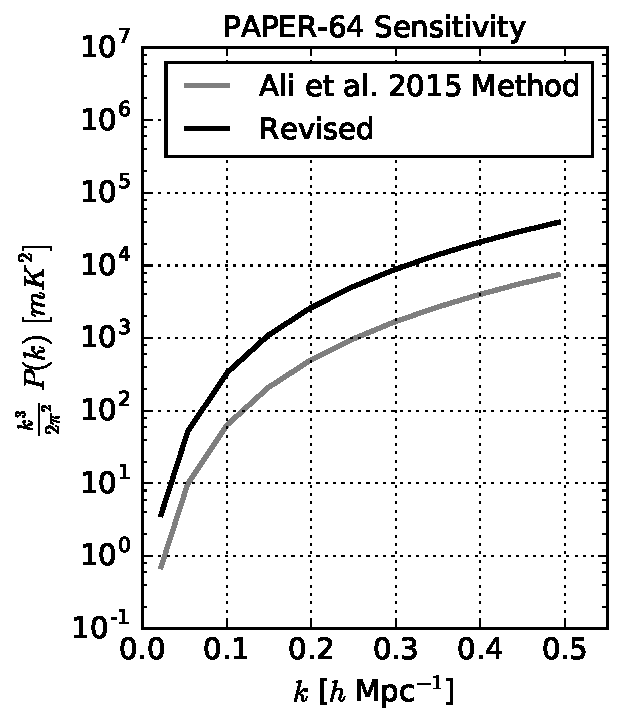
\includegraphics[width=\columnwidth]{plots/sense_check.pdf}
	\caption{An updated prediction for the thermal noise level of PAPER-64 data (black) is shown in comparison to previously 
published sensitivity limits (gray), both computed for the analysis methods used in \citetalias{ali_et_al2015}. Major factors that contribute to the discrepancy are $
\Omega_{\rm eff}$, $N_{\rm days}$ and $N_{\rm bls}$, as in Equation \eqref{eq:sense} and described in Section \ref{sec:PSSense}, which when combined decreases our 
sensitivity (higher noise floor) by a factor of $\sim7$ in mK$^{2}$.}
	\label{fig:sense_check}
\end{figure}

To verify our thermal noise prediction, we form power spectra estimates using a pure noise simulation. We create Gaussian 
random noise assuming a constant $T_{\rm rcvr}$ (translated into $T_{\rm sys}$ via Equation \eqref{eq:sys}) but accounting for the true $N_{\rm days}$ as determined 
by LST sampling counts for each time and frequency in the LST-binned data. We convert $T_{\rm sys}$ into a root-mean-square variance statistic 
using:

\begin{equation}
\label{eq:noise}
T_{\rm rms} = \frac{T_{\rm sys}}{\sqrt{\Delta\nu \Delta t N_{\rm days} N_{\rm pols}}},
\end{equation}

\noindent where $\Delta\nu$ is channel spacing, $\Delta t$ is integration time, $N_{\rm days}$ is the number of daily counts for a 
particular time and frequency that went into our LST-binned set, and $N_{\rm pols}$ is the number of polarizations ($2$ for Stokes 
I). This temperature sets the variance of the Gaussian random noise.

Power spectrum results for the noise simulation, which uses our full power spectrum pipeline, are shown in Figure 
\ref{fig:ps_noise}. We highlight that the bootstrapped data (black and gray points, with $2\sigma$ error bars) and thermal noise prediction (solid green) show good agreement, as bootstrapping provides an accurate estimate of the noise variance. However, the limits from the full signal loss framework (weighted and unweighted in red and blue, respectively) are inflated, likely due to the additional inclusion of sample variance that comes from the EoR simulations.

\begin{figure*}
	\centering
	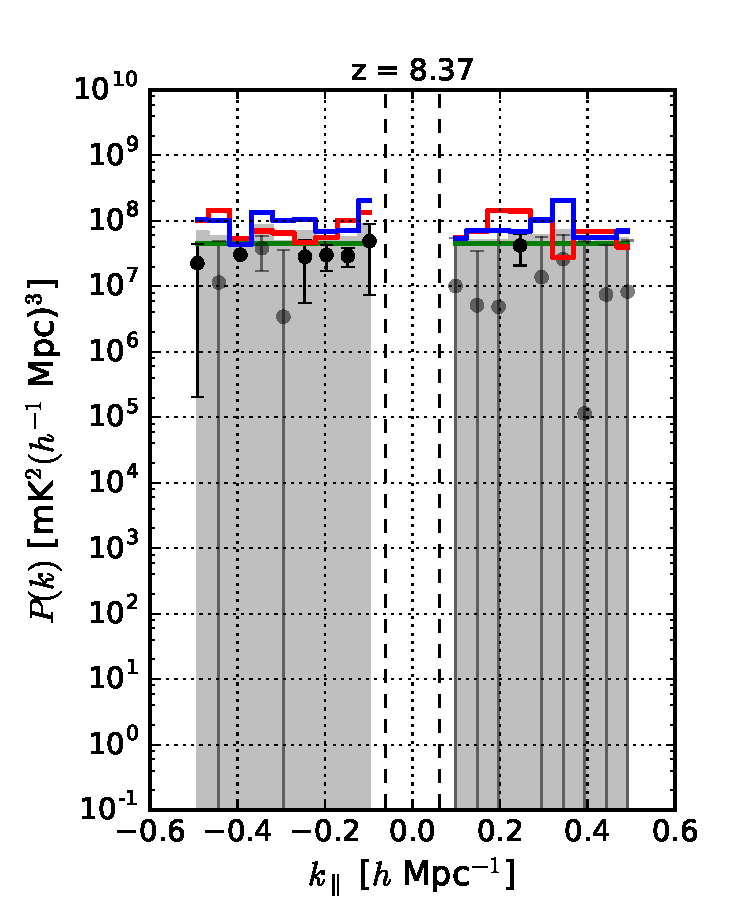
\includegraphics[width=0.4\textwidth]{plots/ps1_noise_add.pdf}
	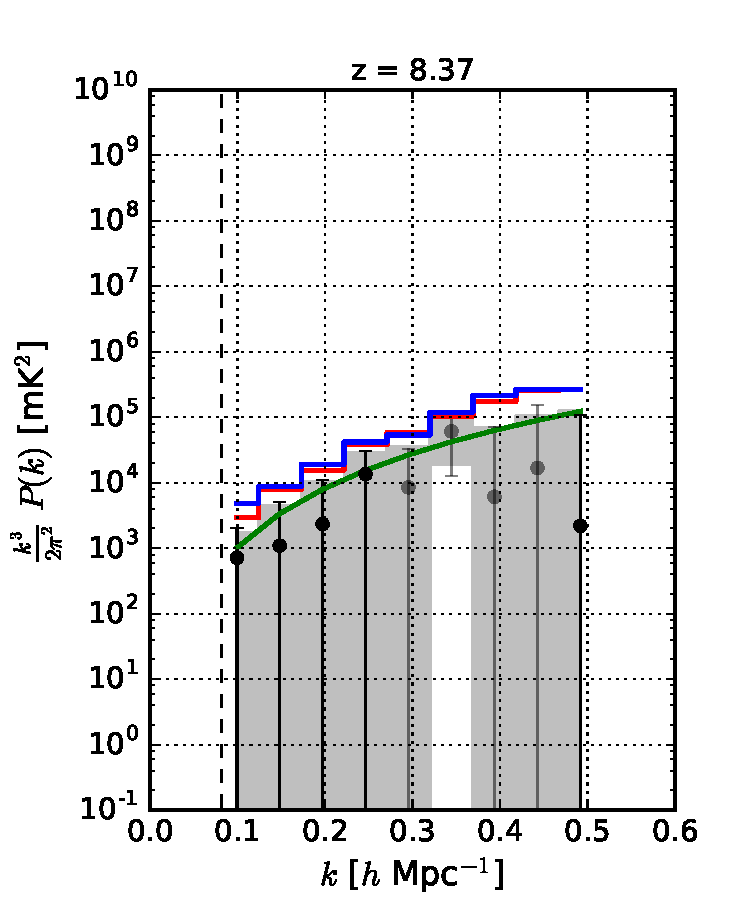
\includegraphics[width=0.4\textwidth]{plots/ps2_noise_add.pdf}
	\caption{The power spectrum for a noise simulation that mimics the noise level of a subset of PAPER-64 data, where the solid red curve is the $2\sigma$ upper limit on the EoR signal estimated from our signal injection framework using $\widehat{\textbf{C}}_{\rm eff}$. The theoretical $2\sigma$ thermal noise level prediction based on observational parameters (calculated by Equation \eqref{eq:sense}) is in green. Additionally, the power spectrum results for the uniform weighted case is shown in three different ways: power spectrum values (black and gray points as positive and negative values, respectively, with $2\sigma$ error bars), the $2\sigma$ upper limit on the EoR signal using our full signal injection framework (solid blue), and the measured power spectrum values with $2\sigma$ thermal noise errors (gray shaded regions). The vertical dashed black lines signify the horizon limit for this analysis using $30$\,m baselines. We highlight that the bootstrapped data points and thermal noise prediction show good agreement, while the limits from the full injection framework are inflated due to the additional inclusion of sample variance that comes from the injection simulations.}
	\label{fig:ps_noise}
\end{figure*}

\subsubsection{Bootstrapping}
\label{sec:Boot}

We bootstrap PAPER-64 power spectra in order to determine confidence intervals for our results. In this section, we highlight 
four specific changes in the way we estimate errors since \citetalias{ali_et_al2015}, the first of which builds off of the lesson we have learned previously about bootstrapping independent samples. 

\begin{itemize}

\item{As discussed in Section \ref{sec:ErrorOverview}, bootstrapping is only a valid way of estimating errors if a dataset is comprised 
of independent samples, or the number of independent samples is well known. The PAPER-64 pipeline outputs $20$ bootstraps (over baselines), each a $2$-dimensional power 
spectrum that is a function of $k$ and time. 

In \citetalias{ali_et_al2015}, a second round of bootstrapping occurred over the time axis. A total of $400$ bootstraps were created in this step 
($N_{\rm boot} = 400$), each comprised of randomly selected values sampled with replacement along the time axis. More 
specifically, each of these bootstraps contained the same number of values as the number of time integrations (which, at $\sim$
$700$, greatly exceeds the approximate number of independent samples after fringe-rate filtering).
Means were then taken of the values in each bootstrap. Finally, power 
spectrum limits were computed by taking the mean and standard deviation over all the bootstraps. We emphasize again that in 
this previous analysis, the number of elements sampled per bootstrap greatly 
exceeded the number of independent LST samples, under-estimating errors. A random draw of $700$ 
measurements from this dataset has many repeated values, and the variance between hundreds ($N_{\rm boot}$) of these random 
samples is smaller than the true underlying variance of the data. 

Given our new understanding of the sensitivity of bootstraps to the number of elements sampled, we have removed the second 
bootstrapping step along time entirely and now simply bootstrap over the baseline axis. Power spectrum $2\sigma$ errors (computed from bootstrap variances) with this bootstrapping change for fringe-rate filtered noise are shown in Figure 
\ref{fig:data_errors}. The estimates are uniformly weighted in order to disentangle the effects of bootstrapping from signal loss. As 
shown in the figure, when more elements are drawn for each bootstrap than the number of 
independent samples (by over-sampling elements along the time axis), repeated values begin to crop up and the apparent variation between bootstraps drops, resulting in limits (gray) below the predicted noise level (green). Using the revised bootstrapping method, where bootstrapping only occurs over the baseline axis, the limits (black) are shown to better agree with the analytic prediction for noise. While Figure \ref{fig:data_errors} implies that errors are under-estimated by a factor of $\sim$ $5$ in mK$^{2}$ for the noise simulation, in practice this factor is lower for the case of real data (a factor of $\sim$ $2$ in mK$^{2}$ instead), possibly due to the data being less correlated in time than the fringe-rate filtered noise in the simulation. }%Figure \ref{fig:data_errors} implies that power spectrum upper limits were originally under-estimated by a factor of $\sim$ $5$ in mK$^{2}$. 

\item{A second change to our bootstrapping procedure is that we now bootstrap over baseline cross-products, instead of baselines themselves. In the previous analysis, baselines were bootstrapped prior to forming cross power spectra, and using this particular ordering of operations (bootstrapping, then cross-multiplication) yields variances that have been found to disagree with predicted errors from bootstrapping using simulations. On the contrary, bootstrapping over cross power spectra ensures that we are estimating the variance of our quantity of interest (i.e. the power spectrum). This change, while fundamental in retaining the integrity of the bootstrapping method in general, alters the resulting power spectrum errors by factors of $<2$ in practice.}

\item{In \citetalias{ali_et_al2015}, individual baselines were divided into $5$ independent groups, where no baselines were repeated in each group. Then, baselines within each group were averaged together, and the groups were cross-multiplied to form power spectra. This grouping method was used to reduce computational time, however upon closer examination it has been found that the initial grouping introduces an element of randomness into the final measurements --- more specifically, the power spectrum value fluctuates depending on how baselines are assigned into their initial groups. Our new approach removes this element of randomness at the cost of computational expense, as we now perform all baseline cross-products.}

\item{Finally, the last change from the \citetalias{ali_et_al2015} method is that our power spectrum points (previously computed as the mean of all bootstraps), are now computed as the power spectrum estimate resulting from not bootstrapping at all. More specifically, we compute one estimate without sampling, and this estimate is propagated through our signal loss computation (this estimate is $\widehat{\textbf{P}}_{x}$). The difference between taking the mean of the bootstrapped values and using the estimate from the no-bootstrapping case is small, but doing the latter ensures that we are forming results that reflect the estimate preferred by all our data.}

\end{itemize}

\begin{figure}
	\centering
	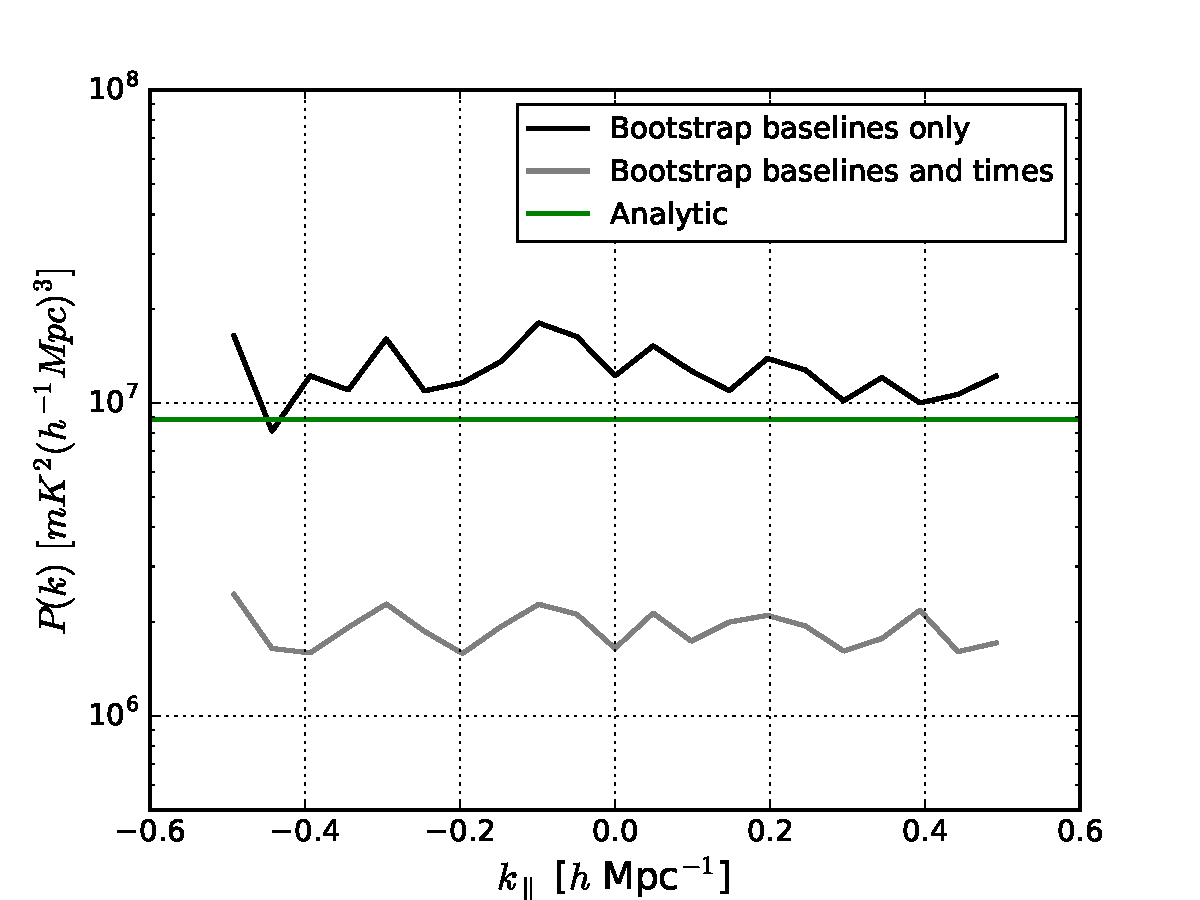
\includegraphics[trim={0.3cm 0cm 0.3cm 0.3cm},width=\columnwidth]{plots/noise_errors.pdf}
	\caption{$2\sigma$ power spectrum errors (from bootstrap variances) for a noise simulation (computed via Equation \eqref{eq:noise} using PAPER-64 observing parameters) using two different bootstrapping 
methods. The noise is fringe-rate filtered and a weighting matrix of $\textbf{I}$ (uniform-weighted) is used in order to disentangle the 
effects of bootstrapping from signal loss. The bootstrapping method used in \citetalias{ali_et_al2015} is shown in gray, where bootstrapping occurs along both the baseline and time axes. This under-estimates errors by sampling more values than independent ones in the dataset (fringe-rate filtering reduces the number of independent samples along time). We use the method illustrated by the black curve in our updated analysis, where bootstrapping only occurs along the baseline axis. We find that these revised limits better agree with the $2\sigma$ analytic prediction for noise (green).}
	\label{fig:data_errors}
\end{figure}

% SECTION 3 BIAS ---------------------------------------------------------------------------------

\subsection{PAPER-64: Bias}
\label{sec:Bias}

In Section \ref{sec:BiasOverview} we highlighted some common sources of bias that can show up as power spectrum 
detections and imitate an EoR signal. We discussed the importance of using jackknife and null tests for instilling confidence in an EoR 
detection, as well as identifying other sources of biases. Here we demonstrate methods used by PAPER-64 to mitigate 
foreground and noise bias and we perform null tests in order to characterize the stability and implications of our results.

\subsubsection{Mitigating Bias}
\label{sec:MitBias}

We briefly discuss one way we mitigate foreground leakage in a power spectrum estimate, and two ways we 
suppress noise biases. These methods are not novel to this analysis but here we frame them in the context of minimizing false 
(non-EoR) detections. 

Tailoring window functions is one way to suppress foreground biases (similar discussions to the following one are in \citet{liu_et_al2014b} and \citetalias{ali_et_al2015}). As alluded to in Section \ref{sec:SiglossOverview}, we 
have a choice for the normalization matrix $\textbf{M}$ in Equation \eqref{eq:phat}. For the analysis of PAPER-64 data, we 
compute $\textbf{M}$ using the matrix $\textbf{F}$ (chosen because this would be the Fisher matrix if $\textbf{R} \equiv \textbf{C}^{-1}$), defined as:

\begin{equation}
\textbf{F}_{\alpha\beta} = \frac{1}{2} \text{tr} [\textbf{R}\textbf{Q}^{\alpha}\textbf{R}\textbf{Q}^{\beta} ]
\end{equation}

\noindent where $\textbf{R}$ is the data-weighting matrix and $\alpha$ and $\beta$ are wavebands in $k_{\parallel}$. We take 
the Cholesky decomposition of $\textbf{F}$, decomposing it into two lower triangular matrices (which is possible since $\textbf{F}$ is Hermitian):

\begin{equation}
\textbf{F} = \textbf{LL}^{\dagger}.
\end{equation}

\noindent Next, we construct $\textbf{M}$:

\begin{equation}
\textbf{M} = \textbf{DL}^{-1}
\end{equation}

\noindent where $\textbf{D}$ is a diagonal matrix. In doing so, our window function, defined as $\textbf{W} = \textbf{MF}$, 
becomes:

\begin{equation}
\textbf{W} = \textbf{DL}^{\dagger}.
\end{equation}

\noindent Because of the nature of the lower triangular matrix, this window function has the property of preventing the leakage 
of foreground power from low-$k$ to high-$k$ modes. Specifically, we order the elements in $\textbf{F}$ in such a way so that 
power can leak from high-$k$ modes to low-$k$ modes, but not vice versa. Since most foreground power shows up at low-$k$'s, this method ensures a window function that retains clean, noise-dominated measurements while minimizing the 
contamination of foreground bias. This tailored window function was used in the \citetalias{ali_et_al2015} analysis, however throughout this paper, we use a diagonal $\textbf{M}$ for simplicity.

In addition to mitigating foreground bias at high-$k$'s, two other sources of bias that we actively suppress in the PAPER-64 
analysis are noise bias associated with the squaring of thermal noise and noise bias from crosstalk. In order to avoid the 
former, we filter out certain cross-multiplications when forming $\widehat{q}$ in Equation \eqref{eq:qhat}. Namely, the PAPER-64 
dataset is divided into two halves: even Julian dates and odd Julian dates. Our data vectors are then $\textbf{x}_{even, 1}$ for 
the ``even" dataset and baseline $1$, $\textbf{x}_{odd, 1}$ for the ``odd" dataset and baseline $1$, etc. We only form 
$\widehat{q}$ when the two copies of $\textbf{x}$ come from different groups and baselines, never multiplying ``baseline 1" with ``baseline 1", for 
example, in order to prevent the squaring of the same thermal noise. 

To mitigate crosstalk bias, which appears as a static bias in time, we apply a fringe-rate filter that suppresses fringe-rates of 
zero. Figure \ref{fig:frp} shows that the filter response is zero for such static signals. The effect of filtering out zero fringe-rates 
on power spectrum results is shown in \citetalias{ali_et_al2015}. Most notably, even without accounting for signal loss, the crosstalk bias at all $k$'s is very strong compared to the removed case.

\subsubsection{Jackknife/Null Tests}

As shown in Figure \ref{fig:ps1_data}, our illustrative PAPER-64 power spectrum shows biases above the predicted noise level, particularly at low-$k$ values. As discussed in Section \ref{sec:BiasTypes}, this bias is
most likely attributable to foreground leakage. %The cause for biases at higher $k$-values is more difficult to pinpoint. 

Here we perform three null tests on PAPER-64 data that aim to isolate systematics in the data and verify 
that our biases are not attributable to EoR. Similar to in Section \ref{sec:JackknifeOverview}, we take jackknives along different axes of the dataset to produce multiple power spectra. We then difference them (i.e. the null test) to tease out excess variances.

The three results are shown in Figure \ref{fig:null}. Each test displays the differenced power spectrum between two halves of a jackknife, where the plotted points are the differenced power spectrum values, and the plotted errors are the bootstrapped errors of the two dataset halves added in quadrature. The expected thermal noise level (gray shaded regions) is the thermal noise of each dataset added in quadrature as well. Constructing the tests as such ensures that we are probing whether the variances of each dataset differ by an amount consistent with the thermal noise. We use uniform weightings for all tests. 

We take jackknives along three different axes:

\begin{itemize}
%\item Original Data (black): This is identical to the unweighted, revised PAPER-64 power spectrum in Figure \ref{fig:ps1_data} (one baseline type only) with weighting matrix $\textbf{I}$. There are clear detections at low $k$'s.
\item Baselines: We split our dataset into two halves, where each contains half of the total baselines used in the 
analysis. No baselines are repeated between the two datasets.
\item Sidereal Hour: We split our dataset into two halves based on LST, namely the first half (LSTs 0.5-4.5 hours) and second half (LSTs 
4.5-8.6 hours).
\item Day: We split our dataset into even and odd Julian dates. We form power spectra for each separately, allowing the cross-multiplication of ``even" with ``even", for example, for this null test only. If the same sky signal is in both the ``even" and ``odd" datasets, we expect it to cancel out. %However, allowing these cross-multiplications can in practice introduce a low level noise bias... 
\end{itemize}


\begin{figure*}
	\centering
	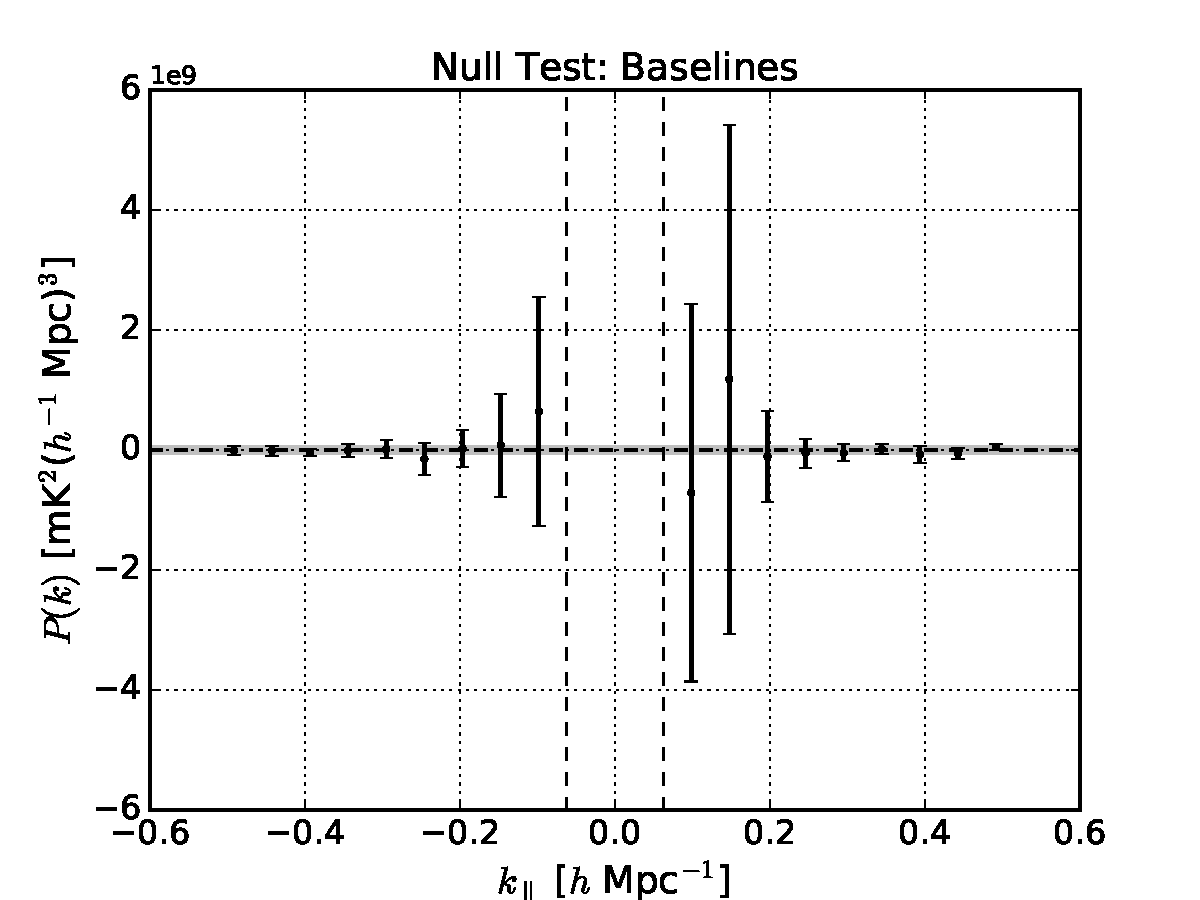
\includegraphics[width=0.47\textwidth]{plots/null_bls.pdf}
	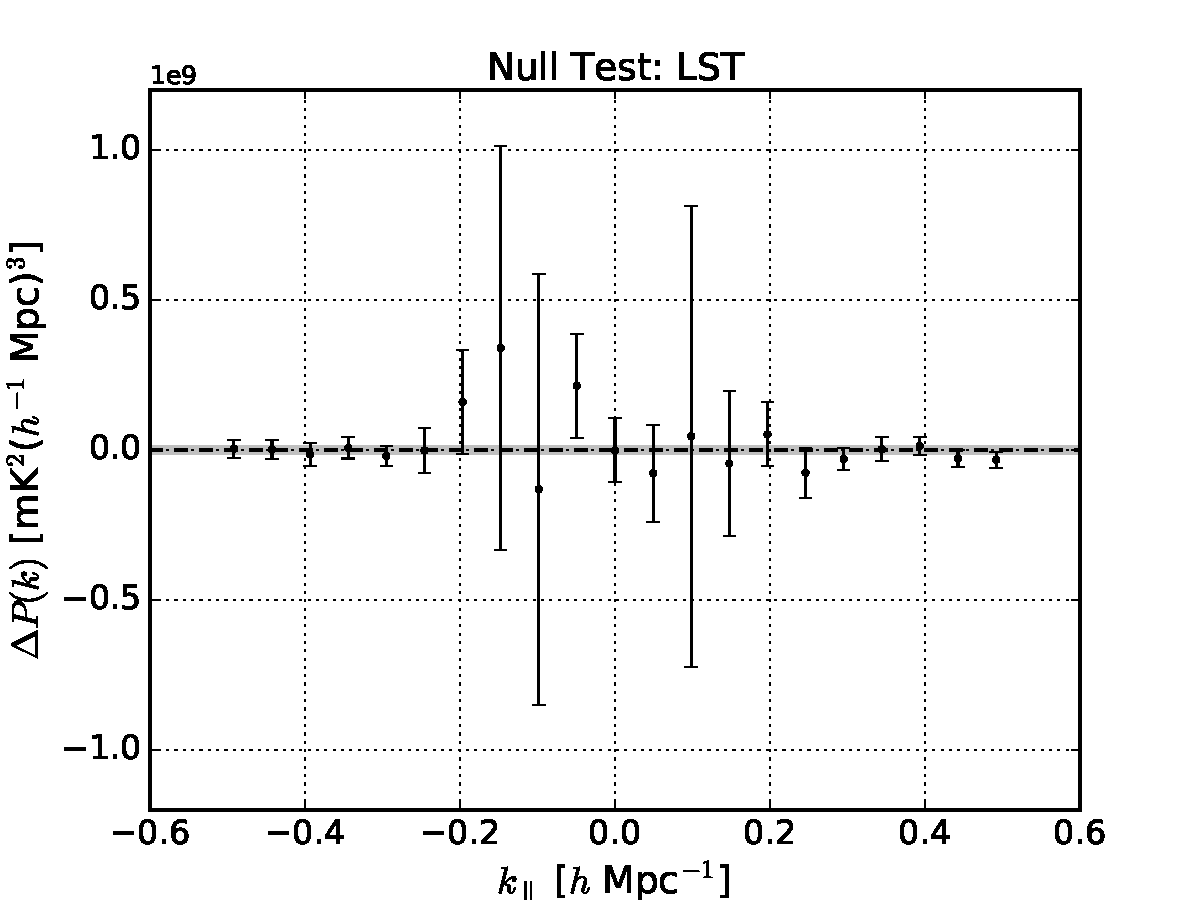
\includegraphics[width=0.47\textwidth]{plots/null_lsts.pdf}
	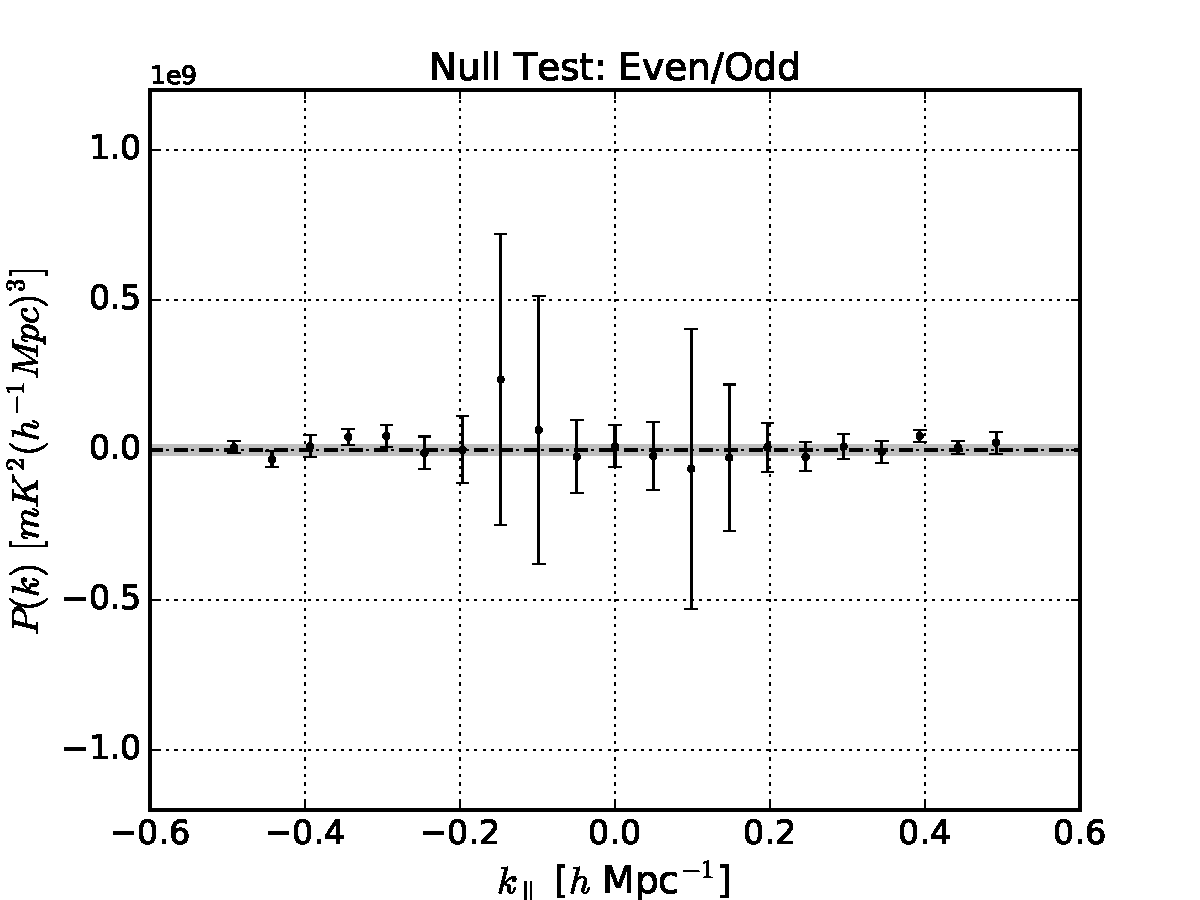
\includegraphics[width=0.47\textwidth]{plots/null_eo.pdf}
	\caption{Differenced power spectrum results (with $2\sigma$ bootstrapped errors) for three null tests, where a jackknife is taken along the baseline axis (top left), LST axis (top right), and even/odd Julian date axis (bottom). The results shown are unweighted (no signal loss), where the power spectrum values plotted are computed from the difference between two power spectra produced on either side of the jackknife axis. The gray shaded region in each plot is the estimated $2\sigma$ theoretical noise limit given the parameters of each test. We find that there are no significant systematics for $k > \pm 0.2$\,$h$ Mpc$^{-1}$ for all three tests. However, we find that all tests exhibit an extra variance at $k$-values near the horizon ($k\sim\pm 0.1$\,$h$ Mpc$^{-1}$), likely due to foreground-noise coupling terms when foregrounds are brightest. Additionally, we find that the LST null test is not fully consistent with zero, implying a bias that is LST dependent and likely caused by varying foregrounds.}
	\label{fig:null}
\end{figure*}

%\begin{figure*}
%	\centering
%	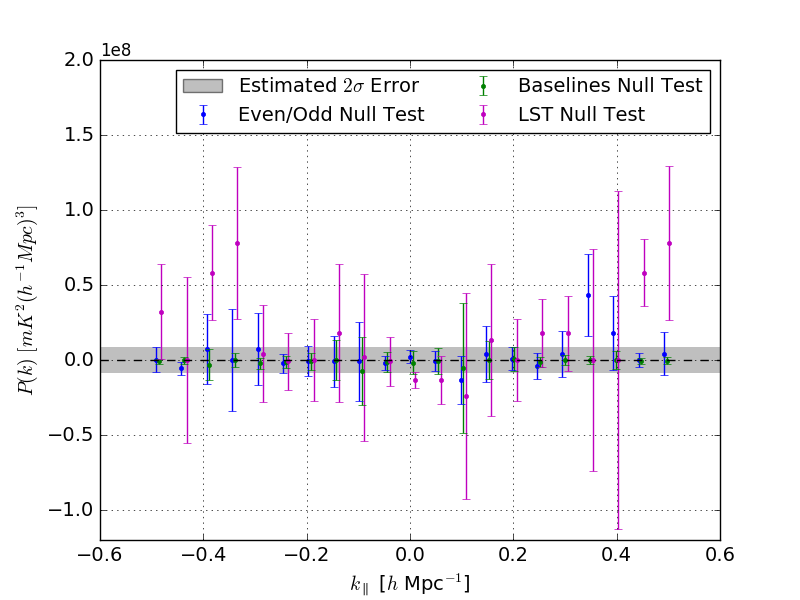
\includegraphics[width=1\textwidth]{plots/null_zoom.png}
%	\caption{Power spectrum results for three null tests using $\widehat{\textbf{C}}_{\rm eff}$, compared to the analytically estimated 
%$2\sigma$ error (gray shaded region). For each of the tests, we take a jackknife along a different axis of the dataset - along Julian days (separating 
%even and odd days; blue), along baselines (green), and along LST (magenta). We expect the sky signal to disappear for a `passing' null test.
%We find that the baselines (green) and even/odd (blue) tests are consistent with noise, and that the dominant source of the biases in our power spectrum are likely caused by variation of foregrounds in LST (due to the magenta result being the most inconsistent with noise)}
%	\label{fig:null}
%\end{figure*}

In investigating Figure \ref{fig:null}, we focus on three main possibilities --- whether the data points and error bars are consistent with thermal noise (``passing"), whether the error bars are consistent with zero but not consistent with thermal noise (``passing but has an additional variance"), or whether the error bars are not consistent with zero at all (``failing"). We examine each case in the context of our results below.

Firstly, all three null tests display data points that lie within the thermal noise gray band for $k > \pm 0.2$\,$h$ Mpc$^{-1}$. In addition, all three null tests show error bars consistent with the thermal noise level for those same $k$'s. This implies that the two jackknife halves do not differ by an amount greater than the thermal noise (i.e. the baselines making up the two jackknives either do not contain bias, or contain similar amounts of bias; we suspect it is the former though more thorough jackknives along this axis are needed to make this conclusion). We deem these as ``passing" null tests for the specific jackknives taken (again, dividing up the data in a different way along the same axes may not yield the same results, so more thorough testing is needed to be sure).

The second null test possibility (error bars consistent with zero but not with thermal noise) is displayed by the $k$-values just outside the horizon ($k\sim\pm 0.1$\,$h$ Mpc$^{-1}$) for all three tests. This indicates an additive noise component that is increasing our errors. More specifically, although we expect each cross-multiplication that is used in power spectrum estimation to have independent noise, there is still the possibility of a noise-foreground coupling term that can introduce power. This is because cross-multiplications produce four additive terms --- a signal-squared term (where signal includes both foregrounds and EoR), two cross-terms between the signal and noise, and one noise-only term. When differencing two power spectra (each with their own four terms), we expect the signal-only term to subtract out for a ``passing" null test, and we expect the noise-only terms to be consistent with thermal noise. While the cross-terms have a mathematical expectation value of zero, in practice we are limited by our number of samples ($90$ cross-products for this analysis times $\sim$ $8$ independent LST samples). Combined with the fact that the foregrounds are so bright, the finite ensemble of the couplings can introduce extra variance that varies with foreground strength. It is therefore not surprising that this effect is largest at $k$-values just outside the horizon, where we expect foregrounds to be brightest post-delay filtering.

Lastly, a third null test result is an error bar not consistent with zero. This is the case for the LST null test at $k\sim-0.15$\,$h$ Mpc$^{-1}$ and $k\sim-0.2$\,$h$ Mpc$^{-1}$. In such a case, the two jackknife halves differ by an amount greater than the thermal noise (i.e. the data point is not in the thermal noise band), yet they are each constrained tightly by individual error bars that when combined, are not consistent with zero. This result implies that there exists a low level bias that is LST-dependent, and likely caused by residual foregrounds that vary in LST. Again, it is not surprising that this type of bias occurs near the horizon limit.

%Most importantly, a clean detection of EoR would have passed all three tests, which is clearly not what we see. 

%We also note that all three tests, whether biased or unbiased, result in power spectrum errors that are slightly larger than the estimated thermal noise (gray band) at high-$k$. This indicates an additive noise component that is increasing our errors (while not affecting whether they pass through zero or not). 

%There are a couple possible explanations for this. Although we expect each cross-multiplication that is used in power spectrum estimation to have independent noise, there is still the possibility of a noise-foreground coupling term that can introduce power. This is because cross-multiplications produce four additive terms --- a signal-squared term (where signal includes both foregrounds and EoR), two cross-terms between the signal and noise, and one noise-only term. When differencing two power spectra, we expect the signal-only term to subtract out for a ``passing" null test, and we expect the noise-only terms to be consistent with thermal noise. The cross-terms, however, can introduce extra variance that would vary with foreground strength, therefore being consistent with the shape of our results.  One additional explanation, specifically for the slightly large error bars seen at high $k$'s, could simply be that our estimate of the thermal noise is too low, as all three tests seem to imply a larger, but consistent, estimate in this high-$k$ regime. Regardless of a potentially larger thermal noise prediction, however, the large error bars near the horizon limit still signify the presence of excess variance in our data.

In this section we have presented the first jackknife and null tests from the PAPER experiment. Unsurprisingly, they imply that our measurements are biased by foregrounds, and not the EoR signal (a clean detection of EoR would have passed all three tests). While simple, these tests outline a framework that can be used by future measurements. The 21\,cm community is beginning to recognize the importance of these types of tests (\citealt{pober_et_al2016b}) in characterizing power spectra at the EoR level, and it is clear that future results will require more substantial and thorough investigations of this nature.

%, and that the even/odd test is consistent with noise given the $2\sigma$ expectations (nearly $95\%$ of the error bars are passing through zero). We additionally note that the error bars for the baselines test (green) are especially small --- this is because the signal is effectively cancelled out prior to cross-multiplication (when forming baseline groups). 

%The null test in LST is much more illuminating. Because of the large variable error bars, many of which do not include zero, this suggests that the primary systematic driving our power spectrum points and errors to be outside the 
%estimated error region is LST-dependent, and therefore likely to be residual foregrounds. In other words, the fact that several magenta power spectrum points, as well as their error bars, are outside the estimated error region implies that $t_{1}$ and 
%$t_{2}$ differ by an amount greater than thermal noise and they do not effectively cancel out the sky signal during cross-multiplication. We also note that the LST null test is biased high, consistent with the interpretation that our positive power spectrum detections in Figure \ref{fig:ps1_data} are those of foregrounds.

%We do not investigate the detailed nature of the residual foregrounds in this paper, though one could imagine performing many 
%similar null tests with a sliding window of $t_{1}$'s and $t_{2}$'s. This would illuminate the particular LST range that introduces 
%the foreground bias (or whether the bias is constant in LST), and could potentially be traced to an individual bright radio source. 
%This type of detailed analysis will be critical at EoR sensitivities; however, for our current analysis we are not surprised that the main source of
%bias we see comes from foregrounds. % in regions where we expect leakage.

% CONCLUSION ---------------------------------------------------------------------------------

\section{Conclusion}
\label{sec:Con}

Although current 21\,cm published power spectrum upper limits lie several orders of magnitude above predicted EoR levels, 
ongoing analyses of deeper sensitivity datasets from PAPER, MWA, and LOFAR, as well as next generation instruments like 
HERA, are expected to continue to push towards EoR sensitivities. As the field progresses towards a detection, we have shown 
that it is crucial for future analyses to have a rigorous understanding of signal loss in an analysis pipeline, be able to accurately 
and robustly calculate both power spectrum and theoretical errors, and consistently undergo a comprehensive set of jackknife 
and null tests.

In particular, in this paper we have investigated the subtleties and tradeoffs of common 21\,cm power spectrum techniques on 
signal loss, error estimation, and bias, which can be summarized as follows:

\begin{itemize}
\item Substantial signal loss can result when weighting data using empirically estimated covariances (Section 
\ref{sec:SiglossOverview}). Loss of the 21\,cm signal is especially significant the fewer number of independent modes that
exist in the data. Hence, there exists a trade-off between sensitivity driven 
time-averaging techniques such as fringe-rate filtering and signal loss when using empirically estimated covariances. 
\item Signal injection and recovery simulations can be used to quantify signal loss (Section \ref{sec:Sigloss}). However, a 
signal-only simulation (i.e. comparing a uniformly weighted vs. weighted power spectrum of EoR only) can under-estimate loss by 
failing to account for correlations between the data and signal (Section \ref{sec:siglossmethod}).
\item Errors that are estimated via bootstrapping can be under-estimated if samples in the dataset are significantly correlated 
(Section \ref{sec:ErrorOverview}). However, if the number of independent samples in a dataset is well-determined, bootstrapping is a 
simple and accurate way of estimating errors.
\item Meaningful null tests are vital to validate an EoR detection (Section \ref{sec:JackknifeOverview}). Similarly, performing 
jackknife tests along multiple axes of a dataset is necessary for confidence in an EoR detection and can also be used to tease 
out systematics.
\end{itemize}

As a consequence of our investigations, we have also used a subset of PAPER-64 data to make a new power spectrum analysis. This serves as an illustrative example of using a signal injection framework, correctly computing errors via bootstrapping, accurately estimating thermal noise, and implementing jackknife tests. Our revised PAPER-64 limits are presented in Kolopanis et al. (\textit{submitted}), which supersede all previously published PAPER limits. The main reasons for a previously under-estimated limit and 
ways in which our new analysis differs can be summarized by the following:

\begin{itemize}
\item Signal loss, previously found to be $<2\%$ in \citetalias{ali_et_al2015}, was under-estimated by a factor of $>$$1000$ for empirically estimated inverse 
covariance weighting. Using a regularized covariance weighting method can minimize loss (Section 
\ref{sec:Weight}), however, because a regularized weighting method is not as aggressive as the former, our results are still a 
factor of $\sim10$ in mK higher than the lossy empirical inverse covariance limits. Under-estimated signal loss therefore represents the bulk of our revision. 
This revision is similar to the re-analysis of results from the GMRT (\citealt{paciga_et_al2013}) which were also 
revised from new signal loss calculations associated with their singular value decomposition foreground filter.
\item Power spectrum errors, originally computed by bootstrapping, were under-estimated for the data by a factor of $\sim2$ in mK due to oversampling data whose effective number of independent samples was reduced from fringe-rate filtering (Section \ref{sec:Boot}). 
\item Several factors used in an analytic expression to predict the noise-level in PAPER-64 data were revised, yielding a 
decrease in predicted sensitivity level by a factor of $\sim3$ in mK (Section \ref{sec:PSSense}). We note that our sensitivity prediction is revised by a factor less than our overall
power spectrum result, implying that if taken at face value, the theoretical prediction for noise in \citetalias{ali_et_al2015} was too high for its data 
points.
\end{itemize}

The future of 21\,cm cosmology is exciting, as new experiments have sensitivities that expect to reach and surpass EoR levels, improved 
foreground mitigation and removal strategies are being developed, and simulations are being designed to better understand 
instruments. On the power spectrum analysis side, robust signal loss simulations, precise error calculations, and 
comprehensive jackknife tests will play critical roles in accurate 21\,cm results. With strong foundations being established now, it is safe to say that we can expect to learn much about reionization and our early Universe in the coming years.


% ACKNOWLEDGEMENTS ---------------------------------------------------------------------------------

\section{Acknowledgements}
CC would like to acknowledge the UC Berkeley Chancellor's Fellowship and National Science Foundation Graduate Research 
Fellowship (Division of Graduate Education award 1106400). She would also like to thank Phil Bull, Bryna Hazelton, Miguel Morales, and Eric Switzer for helpful discussions. PAPER and HERA 
are supported by grants from the National Science Foundation (awards 1440343, and 1636646). ARP, DCJ, and JEA would 
also like to acknowledge NSF support (awards 1352519, 1401708, and 1455151, respectively). SAK is supported by the University of Pennsylvania School of Arts and Sciences Dissertation Completion Fellowship. JSD acknowledges NSF AAPF
award 1701536. AL acknowledges support for this work by NASA through Hubble Fellowship grant \#HST-HF2-51363.001-A awarded by the Space Telescope Science Institute, which is operated by the Association of Universities for Research in Astronomy, Inc., for NASA, under contract NAS5-26555. We graciously thank SKA-SA for site infrastructure and observing support.
\label{sec:Ack}

% APPENDIX ---------------------------------------------------------------------------------

\color{blue}

\appendix
\section{A toy model for inverse covariance weighting}
\label{sec:icw_appendix}

%AAAXXX

We illustrate the way in which the quadratic estimator, Equations \eqref{eq:qhat} and \eqref{eq:phat}, is intended to estimate the power spectrum of EoR in the presence of contamination by other terms by considering two simpler, but similar, cases of estimating the variance of data.  We have specifically chosen a toy model where the data covariance is diagonal, as indeed we expect the EoR signal to be.  We assume we have $N$ data points $\Delta_i$ which are the sum of a desired signal $\sigma_i$ and an undesired contaminant $\upsilon_i$
\begin{equation}
\Delta_i = \sigma_i + \upsilon_i
\end{equation}
with 
\begin{equation}
\langle \sigma_i \rangle = 0; \; \langle \sigma^2_i \rangle = s; \; {\rm and}~\langle \bm{\sigma \sigma}^T \rangle = s \mathbf{I}_{N \times N} \equiv \mathbf{S}
\end{equation}
and we wish to estimate $s$.  The contaminant in this case has a similar structure for its covariance, and is assumed uncorrelated with the signal
\begin{equation}
\langle \upsilon_i \rangle = 0; \; 
\langle \upsilon^2_i \rangle = u; \; 
\langle \bm{\upsilon \upsilon}^T \rangle = u \mathbf{I}_{N \times N} \equiv \mathbf{U}; {\rm and}~ 
\langle \sigma_i \upsilon_j \rangle = 0
\end{equation}
With the covariance matrix given by $\C = \mathbf{S} + \mathbf{U}$, the estimator for $s$ using the optimal quadratic estimator prescription is
\begin{equation}
\label{eq:ICWFormula}
\hat{s} = \half {\F}^{-1} \left( \bm{\Delta}^T \invC \PDeriv{\C}{s}  \invC \bm{\Delta} \right) 
\end{equation}
where $\F$ is the Fisher matrix.  
The expectation of the estimator is then
\begin{equation}
\langle \hat{s} \rangle = \frac{\langle \bm{\Delta^T \Delta} \rangle}{N} = s + u
\end{equation}
In this case, the quadratic estimator returns an entirely reasonable result, but, since the covariance of the undesired signal has the same form as the desired signal, that is,
$\PDeriv{\mathbf{S}}{s} = \PDeriv{\mathbf{U}}{u} =  \PDeriv{\C}{s}$, we find that when {\it the covariance structure of the contaminant is identical to the signal}, the information available to the quadratic estimator to distinguish the two is degenerate, and  is only possible to achieve an unbiased estimate of $s$ by using some additional information to estimate the additive bias due to $u$ and subtract it.  In fact, if one uses the standard formula \citep[e.g.][, Equation 6]{dillon14} for the additive bias
\begin{equation}
b = \half \F^{-1} \Tr\left[ (\C - \mathbf{S}) \invC \PDeriv{\C}{s} \invC \right]
\end{equation}
one indeed finds $b = u$.

Now consider a case, chosen to be very similar to the toy model in \ref{sec:toymodel},  in which the data again have an additive contaminant, now given by
\begin{equation}
\Delta_i = \sigma_i + \upsilon m_i
\end{equation}
where the properties of $\sigma_i$ are as before, but now $\upsilon$ is a random variable and $m_i$ is a fixed function of $i$ with
\begin{equation}
\langle \upsilon \rangle = 0; \;
\langle \upsilon^2 \rangle = u; \; 
 \langle \bm{\upsilon \upsilon}^T \rangle = u \mathbf{m m}^T \equiv \mathbf{U}; \;
 \mathbf{m}^T \mathbf{m} = 1; \; {\rm and}~ 
\langle \sigma_i \upsilon \rangle = 0
\end{equation}
Here $\mathbf{m}$ represents a mode which is correlated across many data points (i.e., we are assuming $\mathbf{U}$ need {\it not} be diagonal), with amplitude given by  $\upsilon$.  The normalization of $\mathbf{m}$ is a matter of convention, and can be absorbed in the variance $u$; the choice above will be convenient for understanding the limiting case $u \gg s$.

We can again calculate the estimator given by \eqref{eq:ICWFormula} explicitly by using the Sherman-Morrison identity to invert the covariance matrix.  Defining
\begin{equation}
\xi \equiv \frac{u/s}{1+u/s}
\end{equation} 
we have
\begin{equation}
\invC  =   \frac{1}{s} \left(\I - \xi \mathbf{m m}^T \right)
\end{equation}
Proceeding to calculate the full estimator
\begin{equation}
\hat{s} = \half {\F}^{-1} \left(\bm \Delta^T \invC \PDeriv{\C}{s}  \invC \bm \Delta \right) = \frac{ \bm \Delta^T  (\I +  (\xi^2 - 2 \xi)  \mathbf{m m}^T)  \bm \Delta}{N + \xi^2 - 2 \xi} 
\end{equation}
The expectation is
\begin{equation}
\langle \hat{s} \rangle = 
s + \frac{1 - 2 \xi + \xi^2}{N + - 2 \xi + \xi^2} u 
\end{equation}
It is worth observing immediately that there is no multiplicative bias on $s$, and that the additive bias is strictly $< u/N$.

An instructive limit is $u \gg s$, $\xi \to 1$, in which case the the virtue of weighting by $\invC$ becomes clearer: it becomes
\begin{equation}
\invC  = \frac{1}{s} \left(\I - \mathbf{m m}^T \right)
\end{equation}
where $\I - \mathbf{m m}^T$ is the projection operator, projecting out $\mathbf{m}$ from any any vector it acts on, and further, the linear bias tends to 0 as $\xi \to 1$, i.e., the projection is ``perfect'' and not ``undone'' by the Fisher matrix normalization.

This is indeed the desired behavior of the inverse covariance weighting, where removal of contamination with a known covariance can be suppressed by a kind of projection of the offending modes.  But even in this case, it is worth pointing out that estimator still has a linear bias for finite $u$.  We also assume that the contaminating mode $\mathbf{m}$ is known perfectly; the next appendix takes up the case where the modes are estimated from the data.

We find the following things:
\begin{itemize}

\item If the covariance of residual foreground contamination were known perfectly, and its covariance structure is sufficiently different from the EoR signal, then we can expect a quadratic estimator of the form Equation \ref{} % Need to put the full equation in the main body, I think
to produce an estimate of the EoR power spectrum with a small linear bias, which is always positive, and no multiplicative bias.  If the foregrounds have a very similar covariance structure to the EoR, then this linear bias could be large.  We do have a reasonable expectation of different covariance structure since the foregrounds, before any processing, {\it are} strongly correlated between frequencies.  That is, the OQE with the correct covariance matrix but without linear bias subtraction will always produce an estimate which is {\it high} relative to the true value.

\item While the correct covariance will remove this contamination, there is no particular harm in having these modes be strongly correlated with the data, since we desire their projection in any case.  

\item If the covariance matrix is estimated from the data, the strong correlation between the estimated modes and the data will in general produce an estimate of the signal power spectrum which in general is strongly biased {\it low} relative to the true value.  In this context, this is what we call ``signal loss.'' 

\item The effect of the bias is worsened when the number of independent samples used to estimate the covariance matrix is reduced.

\item The convergence of the modes of the empirical covariance matrix to the true matrix depends on the size of the eigenvalues, with the modes with the largest eigenvalues converging more quickly (in norm) to the true eigenvector than those with smaller eigenvalues.  Thus, in estimating the covariance matrix empirically, larger eigenvalue modes are likely to be more reliable.  

% JEA - I really struggle with whether this is intuitively reasonable ... it's hard to get a sense of what "noise" is averaging down slower.  All modes have the same number of samples going into the estimate.  But the size of he eigenvalue is an estimate of its "signal/noise" in the given data realization? 
% Also, have we shown this sufficiently rigorously?  Is the toy model sufficiently general?  (Probably.)  But, for any dataset you kind of have to make a decision about where you think "reliable" is, i.e., where in eigenvalue would you make a cut?  Is Figure 20 basically trying to argue for the real data that this is ~a few modes?

\end{itemize}

\color{black}

%\appendix
\section{A toy model for signal loss}
\label{sec:sigloss_appendix}

In this Appendix, we examine a toy model for signal loss. Our goal is to derive an analytic formula for power spectrum signal loss. While this 
model does not apply generally to all the scenarios presented in this paper, it provides some analytic intuition for how the coupling between data and an empirical covariance can result in signal loss.

The minimum-variance quadratic estimator $\widehat{P}_\alpha$ for the $\alpha$th bandpower of the power spectrum is given by 
\begin{equation}
\widehat{P}_\alpha = \frac{1} {2 \F_{\alpha \alpha} }\x^t \C^{-1} \Q^{\alpha} \C^{-1} \x,
\end{equation}
where
\begin{equation}
F_{\alpha \alpha} \equiv \frac{1}{2} \textrm{tr} \left( \C^{-1} \Q^\alpha \C^{-1} \Q^\alpha \right)
\end{equation}
is the $\alpha$th diagonal element of the Fisher matrix. For this section only, with no loss of generality, we assume that the data $\textbf{x}$ are real. We also assume for simplicity that $\mathbf{x}$ is the data from a single instant in time, so that it is of length $N_f$, where $N_f$ is the number of frequency channels.

In our case, we do not have \emph{a priori} knowledge of the covariance matrix. Thus, we deviate from the true minimum-variance quadratic estimator and replace $\C$ with $\Chat$, its data-derived approximation. Our estimator then becomes
\begin{equation}
\label{eq:phatloss}
\widehat{P}_\alpha^\textrm{loss} = \frac{1} {2 \widehat{\F}_{\alpha \alpha} }\x^t \Chat^{-1} \Q^{\alpha} \Chat^{-1} \x,
\end{equation}
where
\begin{equation}
\widehat{F}_{\alpha \alpha} \equiv \frac{1}{2} \textrm{tr} \left( \Chat^{-1} \Q^\alpha \Chat^{-1} \Q^\alpha \right),
\end{equation}
with the label ``loss" to foreshadow the fact that this will be an estimator with signal loss (i.e., a multiplicative bias of less than unity). We will now provide an explicit demonstration of this by modeling the estimated covariance as
\begin{equation}
\label{eq:ChatDef}
\Chat = (1-\eta) \C + \eta \x \x^t,
\end{equation}
where $\eta$ is a parameter quantifying our success at estimating the true covariance matrix. If $\eta = 0$, our covariance estimate has perfectly modeled the true covariance and $\Chat = \C$. On the other hand, if $\eta =1$, then our covariance estimate is based purely on the one realization of the covariance that is our actual data, and we would expect a high level of overfitting and signal loss.

Our strategy for computing the signal loss will be to insert Equation \eqref{eq:ChatDef} into Equation \eqref{eq:phatloss} and to express the resulting estimator $\widehat{P}_\alpha^\textrm{loss}$ in terms of $\widehat{P}_\alpha$. We begin by expressing $\Chat^{-1}$ in terms of $\C^{-1}$ using the Woodbury identity so that
\begin{equation}
\Chat^{-1} = \frac{\C^{-1}}{1-\eta} \left[ \I - \frac{\eta \x \x^t \C^{-1}}{1+ \eta (g-1)}\right],
\end{equation}
where we have defined $g \equiv \x^t \C^{-1} \x$. Inserting this into our Fisher estimate we have
\begin{equation}
\widehat{F}_{\alpha \alpha} = \frac{F_{\alpha \alpha}}{(1-\eta)^2} \left[ 1 -\frac{\eta }{1+ \eta (g-1)} \frac{h_{\alpha \alpha}}{F_{\alpha \alpha}} + \frac{1}{2} \left( \frac{\eta }{1+ \eta (g-1)} \right)^2 \frac{h_\alpha^2}{F_{\alpha \alpha}}\right],
\end{equation}
where $h_\alpha \equiv \x^t \C^{-1} \Q^\alpha \C^{-1} \x $ and $h_{\alpha \alpha} \equiv \x^t \C^{-1} \Q^\alpha \C^{-1} \Q^\alpha \C^{-1}\x $. Note that $g$, $h_\alpha$, and $h_{\alpha \alpha}$ are all random variables, since they depend on $\x$. Inserting these expressions into our estimator gives
\begin{equation}
\label{eq:phatlossexpanded}
\widehat{P}_\alpha^\textrm{loss} = \frac{1}{2} \frac{h_\alpha}{F_{\alpha \alpha}} \left[ 1 - \frac{\eta g}{1+ \eta (g-1)}\right]^2  \left[ 1 -\frac{\eta }{1+ \eta (g-1)} \frac{h_{\alpha \alpha}}{F_{\alpha \alpha}} + \frac{1}{2} \left( \frac{\eta }{1+ \eta (g-1)} \right)^2 \frac{h_\alpha^2}{F_{\alpha \alpha}}\right]^{-1}.
\end{equation}
Both for the purposes of analytical tractability and to provide intuition, we expand this expression to leading 
order in $\eta$. This approximates the limiting case where the covariance $\Chat$ is close to the ideal and the 
lossy covariance is a small perturbation.  The result is
\begin{equation}
\widehat{P}_\alpha^\textrm{loss} \approx \frac{1}{2} \frac{h_\alpha}{F_{\alpha \alpha}} \left[ 1 - \eta \left( g - \frac{h_{\alpha \alpha}}{F_{\alpha \alpha}}\right)\right].
\end{equation}
Taking the ensemble average of both sides and noting that the true power spectrum $p_\alpha$ is equal to $\langle h_\alpha \rangle / 2 F_{\alpha \alpha}$, we obtain
\begin{equation}
\langle \widehat{P}_\alpha^\textrm{loss} \rangle \approx (1- \eta N_f) p_\alpha + 4 \eta \frac{\rm{tr} (\C^{-1} \Q^\alpha \C^{-1} \Q^\alpha \C^{-1} \Q^\alpha )}{\left[ \rm{tr} (\C^{-1} \Q^\alpha \C^{-1} \Q^\alpha  ) \right]^2} \approx (1- \eta N_f) p_\alpha,
\end{equation}
where recall that $N_f$ is the length of $\x$, or the number of frequency channels. In the last step we dropped the final term, since it scales as $\eta p_\alpha$ (without the factor of $N$) and is therefore typically small compared to the terms that have been retained.

Recalling that $p_\alpha$ is the \emph{true} power spectrum, one sees that when the covariance in the optimal quadratic estimator is naively replaced by an empirical covariance, the resulting power spectrum estimate is biased low, i.e., there is signal loss. This occurs because of couplings between $\widehat{\C}$ and $\x$, which formally means that what was originally a quadratic estimator is no longer quadratic, but contains higher-order correlations. This violates the assumptions implicit in the derivation of $F_{\alpha \alpha}$ as the normalization factor for converting unnormalized bandpowers $\frac{1}{2} \x^t \C^{-1} \Q^{\alpha} \C^{-1} \x$ into properly normalized power spectrum estimates, where the unnormalized bandpowers are assumed to be two-point (i.e. quadratic) statistics \citep{liu_tegmark2011}. The result is an improperly normalized---and thus lossy---power spectrum estimate.

\section{Derivation of the Jeffreys Prior}
\label{sec:jeffreys}

The Jeffreys prior is an objective, non-informative prior distribution for a parameter space using Bayesian probability (\citealt{jaynes1968}). For the signal injection framework outlined in Section \ref{sec:Practice}, we wish to compute the prior $p(P_{\rm in})$, or the probability density of the power spectrum of the EoR signal. 

The Jeffreys prior is defined as: 

\begin{equation}
\label{eq:jeffreys}
p(P_{\rm in}) \propto \sqrt {\Bigg\langle \Bigg(\frac{\partial \mathcal{L}}{\partial P_{\rm in}} \Bigg)^{2}\Bigg\rangle},
\end{equation}

\noindent where

\begin{equation}
\label{eq:logprob}
\mathcal{L} = \mathrm{ln} \, p(\widehat{P}_{\rm out} | P_{\rm in}),
\end{equation}

\noindent recalling that in our framework $P_{\rm in}$ is the power spectrum of the EoR signal (uniformly weighted), and $\widehat{P}_{\rm out}$ is the weighted output power spectrum of the data plus EoR.

For a single injection amplitude, our bootstrapped $\widehat{P}_{\rm out}$ values are well-approximated by a Gaussian distribution. Simplifying our notation so that $x = P_{\rm in}$ and $y = \widehat{P}_{\rm out}$:

\begin{equation}
\label{eq:prob}
p(y | x) = \frac{1}{\sigma(x) \sqrt{2\pi}} e^{-\frac{1}{2}\big(\frac{y-\bar y(x)}{\sigma}\big)^{2}},
\end{equation}

\noindent where $\sigma$ is the standard deviation of $\widehat{P}_{\rm out}$ and $\bar y$ is the mean of $\widehat{P}_{\rm out}$, and they are both functions of $P_{\rm in}$. Using Equations \eqref{eq:prob} and \eqref{eq:logprob}, the quantity inside the expectation value of Equation \eqref{eq:jeffreys} becomes:

%\begin{equation}
%\label{eq:logprob_full}
%\mathcal{L} = -\, log \, \sqrt{2\pi} - log\, \sigma - \frac{1}{2}\Big(\frac{y-\bar y}{\sigma}\Big)^{2}. 
%\end{equation}

%Next, the quantity inside the expectation value of Equation \eqref{eq:jeffreys} can be computed by taking the derivative of %Equation \eqref{eq:logprob_full} with respect to $P_{\rm in}$, or $x$:

\begin{eqnarray}
\Big(\frac{\partial \mathcal{L}}{\partial x} \Big)^{2} &=& \frac{1}{\sigma^{2}}\Big(\frac{\partial \sigma}{\partial x}\Big)^{2} -  \Big(\frac{2(y-\bar y)}{\sigma^{3}}\Big)\frac{\partial \sigma}{\partial x}\frac{\partial \bar y}{\partial x} - \Big(\frac{2(y-\bar y)^{2}}{\sigma^{4}}\Big)\Big(\frac{\partial \sigma}{\partial x}\Big)^{2} \nonumber \\
&+& \Big(\frac{(y-\bar y)^{2}}{\sigma^{4}}\Big)\Big(\frac{\partial \bar y}{\partial x}\Big)^{2} + \Big(\frac{2(y-\bar y)^{3}}{\sigma^{5}}\Big)\frac{\partial \sigma}{\partial x}\frac{\partial \bar y}{\partial x} + \Big(\frac{(y-\bar y)^{4}}{\sigma^{6}}\Big)\Big(\frac{\partial \sigma}{\partial x}\Big)^{2}.
\end{eqnarray}

Taking the expectation value then removes all terms with odd powers of $(y - \bar y)$ because those Gaussian moments evaluate to 0. Additionally, the second moment can be simplified since $\langle (y - \bar y)^{2} \rangle = \sigma^{2}$ and the fourth moment can be simplified since $\langle (y - \bar y)^{4} \rangle = 3\sigma^{4}$. Finally, after some additional simplification the Jeffreys prior becomes:

\begin{equation}
\label{eq:jeffreys_final}
p(x) \propto \sqrt{ \frac{1}{\sigma^{2}}\Big(2\Big(\frac{\partial \sigma}{\partial x}\Big)^{2} + \Big(\frac{\partial \bar y}{\partial x}\Big)^{2}\Big) }.
\end{equation}

When we simulate our full injection framework as in Section \ref{sec:Practice}, we sample 50 $P_{\rm in}$ values that range from $\sim$$10^{5}$\,mK$^{2}$ ($h^{-1}$ Mpc)$^{3}$ to $\sim$10$^{11}$\,mK$^{2}$ ($h^{-1}$ Mpc)$^{3}$, and we note that the prior is set to zero outside those regions. For the injections that we do sample, we can easily fit analytic functions to the mean and standard deviations of $\widehat{P}_{\rm out}$ ($\bar y$ and $\sigma$) as functions of $P_{\rm in}$. An example of the typical shape of these functions for the PAPER-64 analysis is shown in Figure \ref{fig:jeffreys1}, though we note in practice we fit solutions for every $k$-value and simulation independently.

\begin{figure}
	\centering
	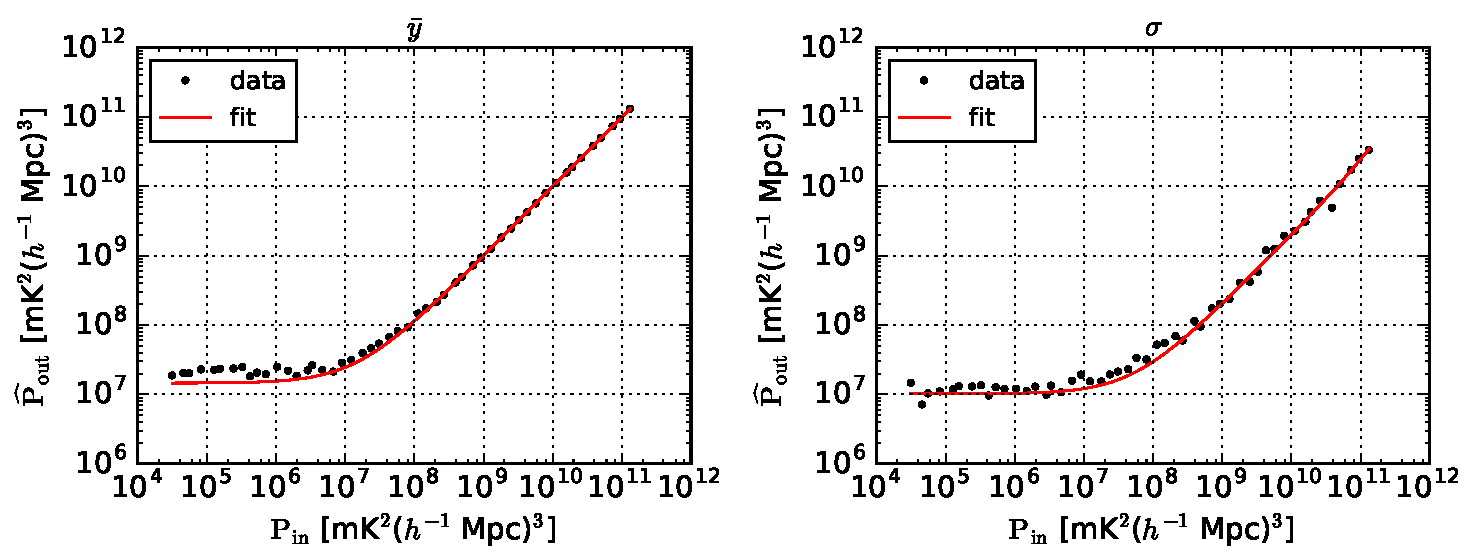
\includegraphics[width=\columnwidth]{plots/jeffrey_fits.pdf}
	\caption{An illustrative example (for the PAPER-64 analysis using uniform weighting and $k=0.393$\,$h$ Mpc$^{-1}$) of how the mean of $P_{\rm out}$ (left) and standard deviation of $P_{\rm out}$ (right) behave as a function of $P_{\rm in}$. Polynomials are fit to each (red) to describe how $\bar y$ and $\sigma$ evolve with $x$ (injection level), respectively, for the computation of the Jeffreys prior as defined in Equation \eqref{eq:jeffreys_final}. The polynomial fits for this example are $y = (-5.1 \times 10^{-15})x^{2} + x + (1.5 \times 10^{7})$ and $y = (5.0 \times 10^{-13})x^{2} + 0.2 x + 10^{7}$ for $\bar y$ and $\sigma$, respectively.}
	\label{fig:jeffreys1}
\end{figure}

We also show the typical shape of the Jeffreys prior used in our analysis in Figure \ref{fig:jeffreys2}, as computed by Equation \eqref{eq:jeffreys_final}. Most noticeably, it is not constant with $P_{\rm in}$, meaning a uniform prior, which is often used for simplicity, is informative in our application. Therefore, due to its objective nature we choose to use a Jeffreys prior in our analysis, multiplying our likelihood functions by Equation \eqref{eq:jeffreys_final} before computing posterior distributions.

\begin{figure}
	\centering
	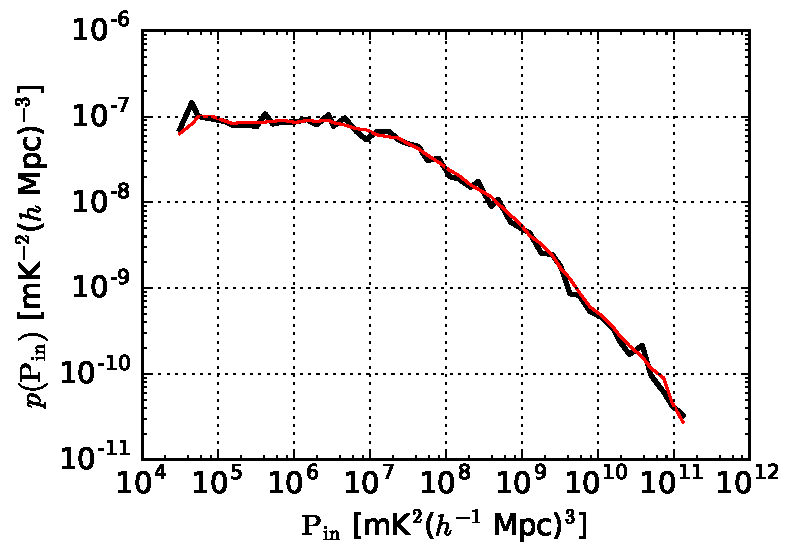
\includegraphics[width=10cm]{plots/jeffrey_prior.pdf}
	\caption{An example of the typical Jeffreys prior shape for the PAPER-64 analysis as computed by Equation \eqref{eq:jeffreys_final} (black). We smooth the prior using a sliding boxcar average for every $5$ injections (red). Most noticeably, the Jeffreys prior is not constant with $P_{\rm in}$, meaning a uniform prior would be an informative prior.}
	\label{fig:jeffreys2}
\end{figure}

%------------------------------- commented below---------------------------------------
\begin{comment}
\section{Simplified Loss Correction}
\label{sec:Pr_appendix}
One of the main difficulties in defining a signal loss procedure is in the interpretation of the injection procedure `output'. The method described in Section \ref{sec:Sigloss} relies on several assumptions which required justification including the assumption that the number of samples is large enough to treat sample variance as a first order purturbation on the ideal covariance matrix instead of the dominant effect we know it is. \acl{I'm not sure the previous sentence was fair. Again, the appendix is a motivating example. Carina's numerical computations do not rely on the derivation.} However it is possible to ask a slightly different question and with less math still get roughly the same answer.

In the main text we made an estimate of the signal loss effecting only the injected EoR by supposing that the lossy injected signal was the difference between the injected and not injected cases: $\widehat{P}_{\rm out} = \widehat{\textbf{P}}_{r} - \widehat{\textbf{P}}_{x}$. Suppose that we rephrase the question we are asking to: ``At what point would an injected signal be detectable at significant levels?". \acl{Can we justify better why this is the right question? In particular, why is the detection of an injected signal the right thing to look at? After all, the universe doesn't do any signal injections. I think to justify that signal injections are the right thing to consider in the first place, one requires some sort of correspondence between equations analogous to Equation \eqref{eq:Deriv1} and \eqref{eq:Deriv2}.} Instead of disentangling the part of the output power spectrum dominated by the injected signal we can simply use $\widehat{\textbf{P}}_{r}$, the weighted power spectrum of the data plus injected signal.
  
\begin{figure}[tp]
\centering
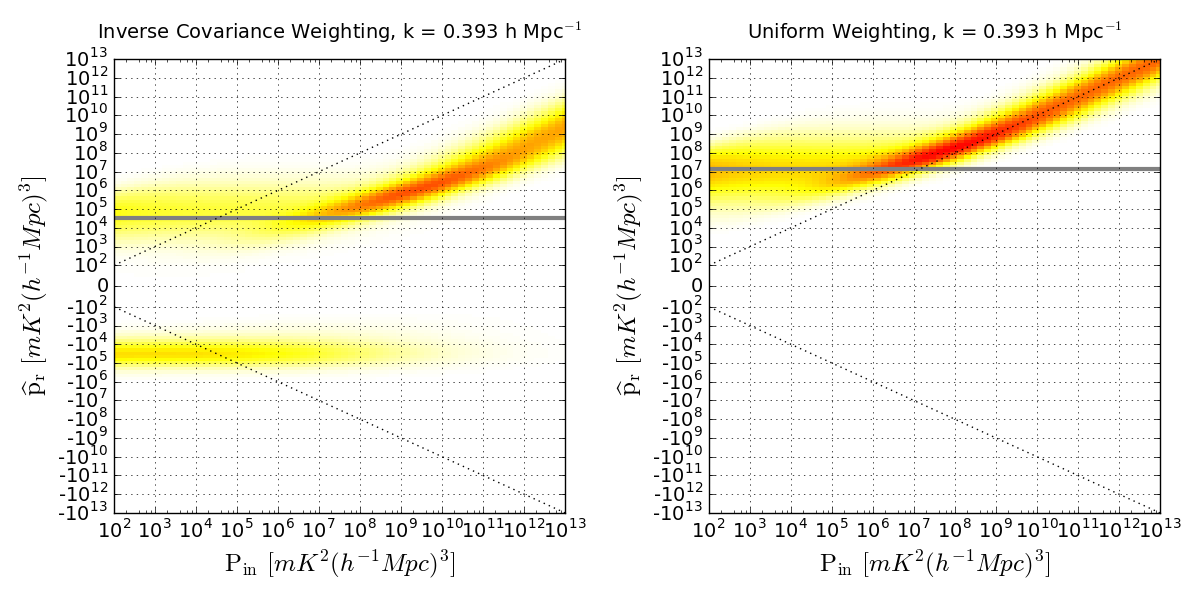
\includegraphics[width=\textwidth]{plots/method2_heatmap_posneg.png}
\caption{The distribution of $\widehat{\textbf{P}}_{r}$ values for a 
given injection level P$_{\rm in}$. The $\widehat{\textbf{P}}_{r}$ values that are plotted on the y-axis represent the weighted power spectrum of data plus the injected signal. It differs from that of Figure \ref{fig:sigloss_transfercurve} by not subtracting off the power spectrum of data alone (not subtracting off the second term in Equation \eqref{eq:sigloss}). We show kernel density estimations of the power spectrum transfer functions as colored heat-maps for the cases of empirical inverse covariance weighted PAPER-64 data (left) and uniform-weighted data (right). The dotted black 
diagonal lines mark a perfect unity mapping, and the solid gray horizontal line denotes the peak of $\widehat{\textbf{P}}_{x}$, the data distribution. At low injection, $\widehat{\textbf{P}}_{r}$ converges to the data level.
}
\label{fig:Pr_vs_Pin}
\end{figure}  
  
This question is phrased visually in Figure \ref{fig:Pr_vs_Pin}. In the 2D space relating total $\widehat{\textbf{P}}_r$ to injected $P_{\rm in}$, very small injected levels begin at the level equivalent of no injection (i.e. data only) and very large levels are dominated by the injected signal. It is the transition zone, where the injected signal amplitude is similar to the data level (and thus subject to cross-correlations in both the covariance and in the power spectrum calculation) that we search for the point at which an injected signal would be clearly detected.
  
\begin{figure}[tp]
\centering
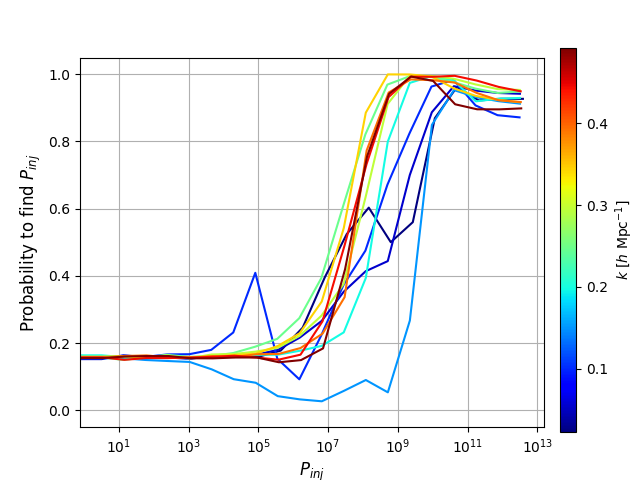
\includegraphics[width=.5\textwidth]{plots/method2_prob_vs_pinj.png}
\caption{The probability that an injected signal of level P$_{\rm inj}$
is observable at a 2$\sigma$ level above the value of $\widehat{\textbf{P}}_{x}$ (data).
The different colors represent different $k$ values. We choose a probability of $95\%$ for our signal loss estimated power spectrum.}
\label{fig:Prob_vs_Pin}
\end{figure}  
  
One difference in this method from the one in the main text is that we are exclusively asking about signals detectable \emph{above} the level of the observed data. Thus it is explicitly limited to placing an upper limit, even if in some $k$-modes one has actual detections above the noise.  This might be seen as more conservative, however, a similar assumption has already been made when choosing to down-weight the data using itself. In such a down-weighting step, one has assumed that significant excess power is associated with a foreground residual. We note that a high SNR detection will require a different method.
  
Formally we can express our test as: ``What is the $P_{\rm in}$ such that the power spectrum of ``data + 
injected eor" ($\widehat{P}_{e+x}$) is detectable above the power spectrum of the data itself ($\widehat{P}_x$. 
In other words, what is $e$ such that,
\begin{equation}
\widehat{\textbf{P}}_{e+x} > \widehat{\textbf{P}}_{x},
\end{equation}  
?''  Of course, both sides of this equation are actually a distribution of values associated with data variance and injected model variance. One way to interpret this test for the two distributions is to compute the probability that the two distributions are not (i.e. the null test) the same.  
 \acl{I'm confused a little by this equation. I would've thought that the right thing to do would be to first compute $x_0$, given implicitly by
 \begin{equation}
 \int_{-\infty}^{x_0}\Prob(\widehat{\textbf{P}}_x) dx = \Lambda,
 \end{equation}
 where $\Lambda$ is the appropriate number for $2\sigma$. That tells us what $x$ would be needed for us to thing that it was an outlier result without there being an extra $e$ in the data. Then we ask how often we get such an outlier result by computing
  \begin{equation}
 \int_{x_0}^\infty \Prob(\widehat{\textbf{P}}_{e+x}|P_{e}) dx.
\end{equation}
Is what you've written equivalent to this? Sorry if this is remedial...
 }
 \begin{equation}
\Prob(P_{e})  =  1 -  \int \Prob(\widehat{\textbf{P}}_x) \Prob(\widehat{\textbf{P}}_{e+x}|P_{e}) x
 \end{equation}
 where $\Prob(\widehat{\textbf{P}}_x)$ is the probability of obtaining the power spectrum $\widehat{\textbf{P}}_x$ found via bootstrapping (power spectrum of data only) and $\Prob(\widehat{\textbf{P}}_{e+x}|P_{e})$ is the probability of obtaining the summed power spectrum $\widehat{\textbf{P}}_{x+e}$ given a range of input power levels, as sampled in Figure \ref{fig:Pr_vs_Pin}.  
 
Probability vs. injection level is shown in Figure \ref{fig:Prob_vs_Pin}. At low injection levels the variation between $\textbf{x}$ and $\textbf{(e+x)}$ is such that the null test is ruled out to within $20$\%. This is the level expected from two distributions with $\sim$10 effective samples. 
As the injected signal approaches the level of the data, the probability of null rejection rises steeply.
  
Lastly, this method requires that we choose the probability at which we choose to reject the null hypothesis. As can be seen in Figure \ref{fig:Prob_vs_Pin}, the difference between $80$\% and $90$\% can mean a difference of almost an order of magnitude in the power spectrum level that is ruled out. We can also see that, due to the small number of samples, the probability does not perfectly converge at high injected power levels. Rather than insist on a rejection at the $99$th percent level, we compromise at $95$\%.

The resulting limits for inverse covariance weighted PAPER-64 data (the same data used in Section \ref{sec:Sigloss}, no regularization), using this second signal loss method, are shown in Figure \ref{fig:sigloss_compare} compared with the method used in the main text. Overall the limits show good agreement, with k modes differing by factors of $\sim$$2$ for $k > 0.1$ $h$Mpc$^{-1}$ .  

\begin{figure}[t]
\centering
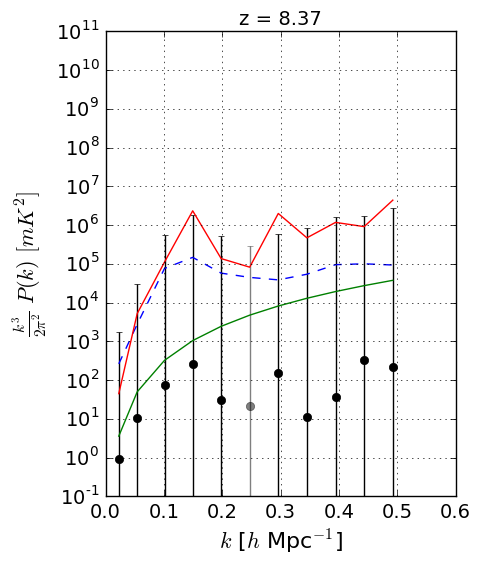
\includegraphics[width=.4\textwidth]{plots/sigloss_method_comparison_95.png}
\caption{A comparison of the signal loss method described in Section \ref{sec:Sigloss}
with the method in this appendix at $95$\% confidence (red curve).
Also shown are the upper limits of the uniform-weighted power spectrum
(blue dashed) and theoretical noise model (green).} 
\label{fig:sigloss_compare} 
\end{figure}

\end{comment}

\bibliographystyle{apj}
\bibliography{refs}

\end{document}

